% **************************************************************************************************************
% A Classic Thesis Style
% An Homage to The Elements of Typographic Style
%
% Copyright (C) 2018 André Miede and Ivo Pletikosić
%
% If you like the style then I would appreciate a postcard. My address
% can be found in the file ClassicThesis.pdf. A collection of the
% postcards I received so far is available online at
% http://postcards.miede.de
%
% License:
% This program is free software; you can redistribute it and/or modify
% it under the terms of the GNU General Public License as published by
% the Free Software Foundation; either version 2 of the License, or
% (at your option) any later version.
%
% This program is distributed in the hope that it will be useful,
% but WITHOUT ANY WARRANTY; without even the implied warranty of
% MERCHANTABILITY or FITNESS FOR A PARTICULAR PURPOSE.  See the
% GNU General Public License for more details.
%
% You should have received a copy of the GNU General Public License
% along with this program; see the file COPYING.  If not, write to
% the Free Software Foundation, Inc., 59 Temple Place - Suite 330,
% Boston, MA 02111-1307, USA.
%
% PLEASE SEE ALSO THE AUTHORS' NOTE REGARDING THIS LICENSE
% IN THE DOCUMENTATION (ClassicThesis.pdf --> Chapter 1 / Chapter01.tex)
% **************************************************************************************************************
\RequirePackage{silence} % :-\
    \WarningFilter{scrreprt}{Usage of package `titlesec'}
    %\WarningFilter{scrreprt}{Activating an ugly workaround}
    \WarningFilter{titlesec}{Non standard sectioning command detected}
\documentclass[ twoside,openright,titlepage,numbers=noenddot,%1headlines,
                headinclude,footinclude,cleardoublepage=empty,abstract=on,
                BCOR=5mm,paper=a4,fontsize=11pt
                ]{scrreprt}

%********************************************************************
% Note: Make all your adjustments in here
%*******************************************************
% ****************************************************************************************************
% classicthesis-config.tex
% formerly known as loadpackages.sty, classicthesis-ldpkg.sty, and classicthesis-preamble.sty
% Use it at the beginning of your ClassicThesis.tex, or as a LaTeX Preamble
% in your ClassicThesis.{tex,lyx} with % ****************************************************************************************************
% classicthesis-config.tex
% formerly known as loadpackages.sty, classicthesis-ldpkg.sty, and classicthesis-preamble.sty
% Use it at the beginning of your ClassicThesis.tex, or as a LaTeX Preamble
% in your ClassicThesis.{tex,lyx} with % ****************************************************************************************************
% classicthesis-config.tex
% formerly known as loadpackages.sty, classicthesis-ldpkg.sty, and classicthesis-preamble.sty
% Use it at the beginning of your ClassicThesis.tex, or as a LaTeX Preamble
% in your ClassicThesis.{tex,lyx} with \input{classicthesis-config}
% ****************************************************************************************************
% If you like the classicthesis, then I would appreciate a postcard.
% My address can be found in the file ClassicThesis.pdf. A collection
% of the postcards I received so far is available online at
% http://postcards.miede.de
% ****************************************************************************************************


% ****************************************************************************************************
% 0. Set the encoding of your files. UTF-8 is the only sensible encoding nowadays. If you can't read
% äöüßáéçèê∂åëæƒÏ€ then change the encoding setting in your editor, not the line below. If your editor
% does not support utf8 use another editor!
% ****************************************************************************************************
\PassOptionsToPackage{utf8}{inputenc}
\usepackage{inputenc}

\PassOptionsToPackage{T1}{fontenc} % T2A for cyrillics
\usepackage{fontenc}


% ****************************************************************************************************
% 1. Configure classicthesis for your needs here, e.g., remove "drafting" below
% in order to deactivate the time-stamp on the pages
% (see ClassicThesis.pdf for more information):
% ****************************************************************************************************
\PassOptionsToPackage{
    drafting=false,    % print version information on the bottom of the pages
    tocaligned=false, % the left column of the toc will be aligned (no indentation)
    dottedtoc=true,  % page numbers in ToC flushed right
    eulerchapternumbers=true, % use AMS Euler for chapter font (otherwise Palatino)
    linedheaders=false,       % chaper headers will have line above and beneath
    floatperchapter=true,     % numbering per chapter for all floats (i.e., Figure 1.1)
    eulermath=true,  % use awesome Euler fonts for mathematical formulae (only with pdfLaTeX)
    beramono=true,    % toggle a nice monospaced font (w/ bold)
    palatino=true,    % deactivate standard font for loading another one, see the last section at the end of this file for suggestions
    style=arsclassica % classicthesis, arsclassica
}{classicthesis}


% ****************************************************************************************************
% 2. Personal data and user ad-hoc commands (insert your own data here)
% ****************************************************************************************************
\newcommand{\myTitle}{Right-angled Coxeter groups are RFRS\xspace}
\newcommand{\mySubtitle}{\xspace}
\newcommand{\myDegree}{\xspace}
\newcommand{\myName}{Niclas Rist\xspace}
\newcommand{\myProf}{Jprof. Dr. Claudio Llosa Isenrich\xspace}
\newcommand{\myOtherProf}{\xspace}
\newcommand{\mySupervisor}{Jprof. Dr. Claudio Llosa Isenrich\xspace}
\newcommand{\myFaculty}{Department of Mathematics\xspace}
\newcommand{\myDepartment}{IAG\xspace}
\newcommand{\myUni}{Karlsruhe Institute of Technology\xspace}
\newcommand{\myLocation}{Karlsruhe, Germany\xspace}
\newcommand{\myTime}{May 16, 2024\xspace}
\newcommand{\myVersion}{\classicthesis}

% ********************************************************************
% Setup, finetuning, and useful commands
% ********************************************************************
\providecommand{\mLyX}{L\kern-.1667em\lower.25em\hbox{Y}\kern-.125emX\@}
\newcommand{\ie}{i.\,e.}
\newcommand{\Ie}{I.\,e.}
\newcommand{\eg}{e.\,g.}
\newcommand{\Eg}{E.\,g.}

\newcommand{\C}{\mathbb{C}} % complex
\newcommand{\R}{\mathbb{R}} % reals
\newcommand{\Q}{\mathbb{Q}} % rationals
\newcommand{\Z}{\mathbb{Z}} % integers
\newcommand{\N}{\mathbb{N}} % natural

\newcommand{\HH}{\mathbb{H}}

\newcommand{\groupp}[2]{\langle#1\;\vert\;#2\rangle}
\newcommand{\abs}[1]{\left\vert #1\right\vert}

\newcommand{\QED}{$\blacksquare$}

\usepackage{amsopn}
\DeclareMathOperator{\spn}{span}
% ****************************************************************************************************


% ****************************************************************************************************
% 3. Loading some handy packages
% ****************************************************************************************************
% ********************************************************************
% Packages with options that might require adjustments
% ********************************************************************
\PassOptionsToPackage{ngerman,american}{babel} % change this to your language(s), main language last
% Spanish languages need extra options in order to work with this template
%\PassOptionsToPackage{spanish,es-lcroman}{babel}
\usepackage{babel}

\usepackage{csquotes}
\PassOptionsToPackage{%
    %backend=biber,bibencoding=utf8, %instead of bibtex
    backend=bibtex8,bibencoding=ascii,%
    language=auto,%
    style=numeric-comp,%
    %style=authoryear-comp, % Author 1999, 2010
    %bibstyle=authoryear,dashed=false, % dashed: substitute rep. author with ---
    sorting=nyt, % name, year, title
    maxbibnames=10, % default: 3, et al.
    %backref=true,%
    natbib=true % natbib compatibility mode (\citep and \citet still work)
}{biblatex}
\usepackage{biblatex}

% \PassOptionsToPackage{fleqn}{amsmath}       % math environments and more by the AMS
\usepackage{amsmath, amssymb, amsthm}

% ********************************************************************
% General useful packages
% ********************************************************************
\usepackage{graphicx} %
\usepackage{scrhack} % fix warnings when using KOMA with listings package
\usepackage{xspace} % to get the spacing after macros right
\PassOptionsToPackage{printonlyused,smaller}{acronym}
\usepackage{acronym} % nice macros for handling all acronyms in the thesis
%\renewcommand{\bflabel}[1]{{#1}\hfill} % fix the list of acronyms --> no longer working
%\renewcommand*{\acsfont}[1]{\textsc{#1}}
%\renewcommand*{\aclabelfont}[1]{\acsfont{#1}}
%\def\bflabel#1{{#1\hfill}}
\def\bflabel#1{{\acsfont{#1}\hfill}}
\def\aclabelfont#1{\acsfont{#1}}
% ****************************************************************************************************
%\usepackage{pgfplots} % External TikZ/PGF support (thanks to Andreas Nautsch)
%\usetikzlibrary{external}
%\tikzexternalize[mode=list and make, prefix=ext-tikz/]
% ****************************************************************************************************


% ****************************************************************************************************
% 4. Setup floats: tables, (sub)figures, and captions
% ****************************************************************************************************
\usepackage{tabularx} % better tables
\setlength{\extrarowheight}{3pt} % increase table row height
\newcommand{\tableheadline}[1]{\multicolumn{1}{l}{\spacedlowsmallcaps{#1}}}
\newcommand{\myfloatalign}{\centering} % to be used with each float for alignment
\usepackage{subfig}
% ****************************************************************************************************


% ****************************************************************************************************
% 5. Setup code listings
% ****************************************************************************************************
\usepackage{listings}
%\lstset{emph={trueIndex,root},emphstyle=\color{BlueViolet}}%\underbar} % for special keywords
\lstset{language=[LaTeX]Tex,%C++,
    morekeywords={PassOptionsToPackage,selectlanguage},
    keywordstyle=\color{RoyalBlue},%\bfseries,
    basicstyle=\small\ttfamily,
    %identifierstyle=\color{NavyBlue},
    commentstyle=\color{Green}\ttfamily,
    stringstyle=\rmfamily,
    numbers=none,%left,%
    numberstyle=\scriptsize,%\tiny
    stepnumber=5,
    numbersep=8pt,
    showstringspaces=false,
    breaklines=true,
    %frameround=ftff,
    %frame=single,
    belowcaptionskip=.75\baselineskip
    %frame=L
}
% ****************************************************************************************************




% ****************************************************************************************************
% 6. Last calls before the bar closes
% ****************************************************************************************************
% ********************************************************************
% Her Majesty herself
% ********************************************************************
\usepackage{classicthesis}


% ********************************************************************
% Fine-tune hyperreferences (hyperref should be called last)
% ********************************************************************
\hypersetup{%
    %draft, % hyperref's draft mode, for printing see below
    colorlinks=false, linktocpage=true, pdfstartpage=3, pdfstartview=FitV,%
    % uncomment the following line if you want to have black links (e.g., for printing)
    %colorlinks=false, linktocpage=false, pdfstartpage=3, pdfstartview=FitV, pdfborder={0 0 0},%
    breaklinks=true, pageanchor=true,%
    pdfpagemode=UseNone, %
    % pdfpagemode=UseOutlines,%
    plainpages=false, bookmarksnumbered, bookmarksopen=true, bookmarksopenlevel=1,%
    hypertexnames=true, pdfhighlight=/O,%nesting=true,%frenchlinks,%
    urlcolor=CTurl, linkcolor=CTlink, citecolor=CTcitation, %pagecolor=RoyalBlue,%
    %urlcolor=Black, linkcolor=Black, citecolor=Black, %pagecolor=Black,%
    pdftitle={\myTitle},%
    pdfauthor={\textcopyright\ \myName, \myUni, \myFaculty},%
    pdfsubject={},%
    pdfkeywords={},%
    pdfcreator={pdfLaTeX},%
    pdfproducer={LaTeX with hyperref and classicthesis}%
}


% ********************************************************************
% Setup autoreferences (hyperref and babel)
% ********************************************************************
% There are some issues regarding autorefnames
% http://www.tex.ac.uk/cgi-bin/texfaq2html?label=latexwords
% you have to redefine the macros for the
% language you use, e.g., american, ngerman
% (as chosen when loading babel/AtBeginDocument)
% ********************************************************************
\makeatletter
\@ifpackageloaded{babel}%
{%
    \addto\extrasamerican{%
        \renewcommand*{\figureautorefname}{Figure}%
        \renewcommand*{\tableautorefname}{Table}%
        \renewcommand*{\partautorefname}{Part}%
        \renewcommand*{\chapterautorefname}{Chapter}%
        \renewcommand*{\sectionautorefname}{Section}%
        \renewcommand*{\subsectionautorefname}{Section}%
        \renewcommand*{\subsubsectionautorefname}{Section}%
    }%
    \addto\extrasngerman{%
        \renewcommand*{\paragraphautorefname}{Absatz}%
        \renewcommand*{\subparagraphautorefname}{Unterabsatz}%
        \renewcommand*{\footnoteautorefname}{Fu\"snote}%
        \renewcommand*{\FancyVerbLineautorefname}{Zeile}%
        \renewcommand*{\theoremautorefname}{Theorem}%
        \renewcommand*{\appendixautorefname}{Anhang}%
        \renewcommand*{\equationautorefname}{Gleichung}%
        \renewcommand*{\itemautorefname}{Punkt}%
    }%
    % Fix to getting autorefs for subfigures right (thanks to Belinda Vogt for changing the definition)
    \providecommand{\subfigureautorefname}{\figureautorefname}%
}{\relax}
\makeatother


% ********************************************************************
% Development Stuff
% ********************************************************************
\listfiles
%\PassOptionsToPackage{l2tabu,orthodox,abort}{nag}
%  \usepackage{nag}
%\PassOptionsToPackage{warning, all}{onlyamsmath}
%  \usepackage{onlyamsmath}


% ****************************************************************************************************
% 7. Further adjustments (experimental)
% ****************************************************************************************************
% ********************************************************************
% Changing the text area
% ********************************************************************
%\areaset[current]{312pt}{761pt} % 686 (factor 2.2) + 33 head + 42 head \the\footskip
%\setlength{\marginparwidth}{7em}%
%\setlength{\marginparsep}{2em}%

% ********************************************************************
% Using different fonts
% ********************************************************************
%\usepackage[oldstylenums]{kpfonts} % oldstyle notextcomp
% \usepackage[osf]{libertine}
%\usepackage[light,condensed,math]{iwona}
%\renewcommand{\sfdefault}{iwona}
%\usepackage{lmodern} % <-- no osf support :-(
%\usepackage{cfr-lm} %
%\usepackage[urw-garamond]{mathdesign} <-- no osf support :-(
%\usepackage[default,osfigures]{opensans} % scale=0.95
%\usepackage[sfdefault]{FiraSans}
% \usepackage[opticals,mathlf]{MinionPro} % onlytext
% ********************************************************************
%\usepackage[largesc,osf]{newpxtext}
%\linespread{1.05} % a bit more for Palatino
% Used to fix these:
% https://bitbucket.org/amiede/classicthesis/issues/139/italics-in-pallatino-capitals-chapter
% https://bitbucket.org/amiede/classicthesis/issues/45/problema-testatine-su-classicthesis-style
% ********************************************************************
% ****************************************************************************************************

% ****************************************************************************************************
% If you like the classicthesis, then I would appreciate a postcard.
% My address can be found in the file ClassicThesis.pdf. A collection
% of the postcards I received so far is available online at
% http://postcards.miede.de
% ****************************************************************************************************


% ****************************************************************************************************
% 0. Set the encoding of your files. UTF-8 is the only sensible encoding nowadays. If you can't read
% äöüßáéçèê∂åëæƒÏ€ then change the encoding setting in your editor, not the line below. If your editor
% does not support utf8 use another editor!
% ****************************************************************************************************
\PassOptionsToPackage{utf8}{inputenc}
\usepackage{inputenc}

\PassOptionsToPackage{T1}{fontenc} % T2A for cyrillics
\usepackage{fontenc}


% ****************************************************************************************************
% 1. Configure classicthesis for your needs here, e.g., remove "drafting" below
% in order to deactivate the time-stamp on the pages
% (see ClassicThesis.pdf for more information):
% ****************************************************************************************************
\PassOptionsToPackage{
    drafting=false,    % print version information on the bottom of the pages
    tocaligned=false, % the left column of the toc will be aligned (no indentation)
    dottedtoc=true,  % page numbers in ToC flushed right
    eulerchapternumbers=true, % use AMS Euler for chapter font (otherwise Palatino)
    linedheaders=false,       % chaper headers will have line above and beneath
    floatperchapter=true,     % numbering per chapter for all floats (i.e., Figure 1.1)
    eulermath=true,  % use awesome Euler fonts for mathematical formulae (only with pdfLaTeX)
    beramono=true,    % toggle a nice monospaced font (w/ bold)
    palatino=true,    % deactivate standard font for loading another one, see the last section at the end of this file for suggestions
    style=arsclassica % classicthesis, arsclassica
}{classicthesis}


% ****************************************************************************************************
% 2. Personal data and user ad-hoc commands (insert your own data here)
% ****************************************************************************************************
\newcommand{\myTitle}{Right-angled Coxeter groups are RFRS\xspace}
\newcommand{\mySubtitle}{\xspace}
\newcommand{\myDegree}{\xspace}
\newcommand{\myName}{Niclas Rist\xspace}
\newcommand{\myProf}{Jprof. Dr. Claudio Llosa Isenrich\xspace}
\newcommand{\myOtherProf}{\xspace}
\newcommand{\mySupervisor}{Jprof. Dr. Claudio Llosa Isenrich\xspace}
\newcommand{\myFaculty}{Department of Mathematics\xspace}
\newcommand{\myDepartment}{IAG\xspace}
\newcommand{\myUni}{Karlsruhe Institute of Technology\xspace}
\newcommand{\myLocation}{Karlsruhe, Germany\xspace}
\newcommand{\myTime}{May 16, 2024\xspace}
\newcommand{\myVersion}{\classicthesis}

% ********************************************************************
% Setup, finetuning, and useful commands
% ********************************************************************
\providecommand{\mLyX}{L\kern-.1667em\lower.25em\hbox{Y}\kern-.125emX\@}
\newcommand{\ie}{i.\,e.}
\newcommand{\Ie}{I.\,e.}
\newcommand{\eg}{e.\,g.}
\newcommand{\Eg}{E.\,g.}

\newcommand{\C}{\mathbb{C}} % complex
\newcommand{\R}{\mathbb{R}} % reals
\newcommand{\Q}{\mathbb{Q}} % rationals
\newcommand{\Z}{\mathbb{Z}} % integers
\newcommand{\N}{\mathbb{N}} % natural

\newcommand{\HH}{\mathbb{H}}

\newcommand{\groupp}[2]{\langle#1\;\vert\;#2\rangle}
\newcommand{\abs}[1]{\left\vert #1\right\vert}

\newcommand{\QED}{$\blacksquare$}

\usepackage{amsopn}
\DeclareMathOperator{\spn}{span}
% ****************************************************************************************************


% ****************************************************************************************************
% 3. Loading some handy packages
% ****************************************************************************************************
% ********************************************************************
% Packages with options that might require adjustments
% ********************************************************************
\PassOptionsToPackage{ngerman,american}{babel} % change this to your language(s), main language last
% Spanish languages need extra options in order to work with this template
%\PassOptionsToPackage{spanish,es-lcroman}{babel}
\usepackage{babel}

\usepackage{csquotes}
\PassOptionsToPackage{%
    %backend=biber,bibencoding=utf8, %instead of bibtex
    backend=bibtex8,bibencoding=ascii,%
    language=auto,%
    style=numeric-comp,%
    %style=authoryear-comp, % Author 1999, 2010
    %bibstyle=authoryear,dashed=false, % dashed: substitute rep. author with ---
    sorting=nyt, % name, year, title
    maxbibnames=10, % default: 3, et al.
    %backref=true,%
    natbib=true % natbib compatibility mode (\citep and \citet still work)
}{biblatex}
\usepackage{biblatex}

% \PassOptionsToPackage{fleqn}{amsmath}       % math environments and more by the AMS
\usepackage{amsmath, amssymb, amsthm}

% ********************************************************************
% General useful packages
% ********************************************************************
\usepackage{graphicx} %
\usepackage{scrhack} % fix warnings when using KOMA with listings package
\usepackage{xspace} % to get the spacing after macros right
\PassOptionsToPackage{printonlyused,smaller}{acronym}
\usepackage{acronym} % nice macros for handling all acronyms in the thesis
%\renewcommand{\bflabel}[1]{{#1}\hfill} % fix the list of acronyms --> no longer working
%\renewcommand*{\acsfont}[1]{\textsc{#1}}
%\renewcommand*{\aclabelfont}[1]{\acsfont{#1}}
%\def\bflabel#1{{#1\hfill}}
\def\bflabel#1{{\acsfont{#1}\hfill}}
\def\aclabelfont#1{\acsfont{#1}}
% ****************************************************************************************************
%\usepackage{pgfplots} % External TikZ/PGF support (thanks to Andreas Nautsch)
%\usetikzlibrary{external}
%\tikzexternalize[mode=list and make, prefix=ext-tikz/]
% ****************************************************************************************************


% ****************************************************************************************************
% 4. Setup floats: tables, (sub)figures, and captions
% ****************************************************************************************************
\usepackage{tabularx} % better tables
\setlength{\extrarowheight}{3pt} % increase table row height
\newcommand{\tableheadline}[1]{\multicolumn{1}{l}{\spacedlowsmallcaps{#1}}}
\newcommand{\myfloatalign}{\centering} % to be used with each float for alignment
\usepackage{subfig}
% ****************************************************************************************************


% ****************************************************************************************************
% 5. Setup code listings
% ****************************************************************************************************
\usepackage{listings}
%\lstset{emph={trueIndex,root},emphstyle=\color{BlueViolet}}%\underbar} % for special keywords
\lstset{language=[LaTeX]Tex,%C++,
    morekeywords={PassOptionsToPackage,selectlanguage},
    keywordstyle=\color{RoyalBlue},%\bfseries,
    basicstyle=\small\ttfamily,
    %identifierstyle=\color{NavyBlue},
    commentstyle=\color{Green}\ttfamily,
    stringstyle=\rmfamily,
    numbers=none,%left,%
    numberstyle=\scriptsize,%\tiny
    stepnumber=5,
    numbersep=8pt,
    showstringspaces=false,
    breaklines=true,
    %frameround=ftff,
    %frame=single,
    belowcaptionskip=.75\baselineskip
    %frame=L
}
% ****************************************************************************************************




% ****************************************************************************************************
% 6. Last calls before the bar closes
% ****************************************************************************************************
% ********************************************************************
% Her Majesty herself
% ********************************************************************
\usepackage{classicthesis}


% ********************************************************************
% Fine-tune hyperreferences (hyperref should be called last)
% ********************************************************************
\hypersetup{%
    %draft, % hyperref's draft mode, for printing see below
    colorlinks=false, linktocpage=true, pdfstartpage=3, pdfstartview=FitV,%
    % uncomment the following line if you want to have black links (e.g., for printing)
    %colorlinks=false, linktocpage=false, pdfstartpage=3, pdfstartview=FitV, pdfborder={0 0 0},%
    breaklinks=true, pageanchor=true,%
    pdfpagemode=UseNone, %
    % pdfpagemode=UseOutlines,%
    plainpages=false, bookmarksnumbered, bookmarksopen=true, bookmarksopenlevel=1,%
    hypertexnames=true, pdfhighlight=/O,%nesting=true,%frenchlinks,%
    urlcolor=CTurl, linkcolor=CTlink, citecolor=CTcitation, %pagecolor=RoyalBlue,%
    %urlcolor=Black, linkcolor=Black, citecolor=Black, %pagecolor=Black,%
    pdftitle={\myTitle},%
    pdfauthor={\textcopyright\ \myName, \myUni, \myFaculty},%
    pdfsubject={},%
    pdfkeywords={},%
    pdfcreator={pdfLaTeX},%
    pdfproducer={LaTeX with hyperref and classicthesis}%
}


% ********************************************************************
% Setup autoreferences (hyperref and babel)
% ********************************************************************
% There are some issues regarding autorefnames
% http://www.tex.ac.uk/cgi-bin/texfaq2html?label=latexwords
% you have to redefine the macros for the
% language you use, e.g., american, ngerman
% (as chosen when loading babel/AtBeginDocument)
% ********************************************************************
\makeatletter
\@ifpackageloaded{babel}%
{%
    \addto\extrasamerican{%
        \renewcommand*{\figureautorefname}{Figure}%
        \renewcommand*{\tableautorefname}{Table}%
        \renewcommand*{\partautorefname}{Part}%
        \renewcommand*{\chapterautorefname}{Chapter}%
        \renewcommand*{\sectionautorefname}{Section}%
        \renewcommand*{\subsectionautorefname}{Section}%
        \renewcommand*{\subsubsectionautorefname}{Section}%
    }%
    \addto\extrasngerman{%
        \renewcommand*{\paragraphautorefname}{Absatz}%
        \renewcommand*{\subparagraphautorefname}{Unterabsatz}%
        \renewcommand*{\footnoteautorefname}{Fu\"snote}%
        \renewcommand*{\FancyVerbLineautorefname}{Zeile}%
        \renewcommand*{\theoremautorefname}{Theorem}%
        \renewcommand*{\appendixautorefname}{Anhang}%
        \renewcommand*{\equationautorefname}{Gleichung}%
        \renewcommand*{\itemautorefname}{Punkt}%
    }%
    % Fix to getting autorefs for subfigures right (thanks to Belinda Vogt for changing the definition)
    \providecommand{\subfigureautorefname}{\figureautorefname}%
}{\relax}
\makeatother


% ********************************************************************
% Development Stuff
% ********************************************************************
\listfiles
%\PassOptionsToPackage{l2tabu,orthodox,abort}{nag}
%  \usepackage{nag}
%\PassOptionsToPackage{warning, all}{onlyamsmath}
%  \usepackage{onlyamsmath}


% ****************************************************************************************************
% 7. Further adjustments (experimental)
% ****************************************************************************************************
% ********************************************************************
% Changing the text area
% ********************************************************************
%\areaset[current]{312pt}{761pt} % 686 (factor 2.2) + 33 head + 42 head \the\footskip
%\setlength{\marginparwidth}{7em}%
%\setlength{\marginparsep}{2em}%

% ********************************************************************
% Using different fonts
% ********************************************************************
%\usepackage[oldstylenums]{kpfonts} % oldstyle notextcomp
% \usepackage[osf]{libertine}
%\usepackage[light,condensed,math]{iwona}
%\renewcommand{\sfdefault}{iwona}
%\usepackage{lmodern} % <-- no osf support :-(
%\usepackage{cfr-lm} %
%\usepackage[urw-garamond]{mathdesign} <-- no osf support :-(
%\usepackage[default,osfigures]{opensans} % scale=0.95
%\usepackage[sfdefault]{FiraSans}
% \usepackage[opticals,mathlf]{MinionPro} % onlytext
% ********************************************************************
%\usepackage[largesc,osf]{newpxtext}
%\linespread{1.05} % a bit more for Palatino
% Used to fix these:
% https://bitbucket.org/amiede/classicthesis/issues/139/italics-in-pallatino-capitals-chapter
% https://bitbucket.org/amiede/classicthesis/issues/45/problema-testatine-su-classicthesis-style
% ********************************************************************
% ****************************************************************************************************

% ****************************************************************************************************
% If you like the classicthesis, then I would appreciate a postcard.
% My address can be found in the file ClassicThesis.pdf. A collection
% of the postcards I received so far is available online at
% http://postcards.miede.de
% ****************************************************************************************************


% ****************************************************************************************************
% 0. Set the encoding of your files. UTF-8 is the only sensible encoding nowadays. If you can't read
% äöüßáéçèê∂åëæƒÏ€ then change the encoding setting in your editor, not the line below. If your editor
% does not support utf8 use another editor!
% ****************************************************************************************************
\PassOptionsToPackage{utf8}{inputenc}
\usepackage{inputenc}

\PassOptionsToPackage{T1}{fontenc} % T2A for cyrillics
\usepackage{fontenc}


% ****************************************************************************************************
% 1. Configure classicthesis for your needs here, e.g., remove "drafting" below
% in order to deactivate the time-stamp on the pages
% (see ClassicThesis.pdf for more information):
% ****************************************************************************************************
\PassOptionsToPackage{
    drafting=false,    % print version information on the bottom of the pages
    tocaligned=false, % the left column of the toc will be aligned (no indentation)
    dottedtoc=true,  % page numbers in ToC flushed right
    eulerchapternumbers=true, % use AMS Euler for chapter font (otherwise Palatino)
    linedheaders=false,       % chaper headers will have line above and beneath
    floatperchapter=true,     % numbering per chapter for all floats (i.e., Figure 1.1)
    eulermath=true,  % use awesome Euler fonts for mathematical formulae (only with pdfLaTeX)
    beramono=true,    % toggle a nice monospaced font (w/ bold)
    palatino=true,    % deactivate standard font for loading another one, see the last section at the end of this file for suggestions
    style=arsclassica % classicthesis, arsclassica
}{classicthesis}


% ****************************************************************************************************
% 2. Personal data and user ad-hoc commands (insert your own data here)
% ****************************************************************************************************
\newcommand{\myTitle}{Right-angled Coxeter groups are RFRS\xspace}
\newcommand{\mySubtitle}{\xspace}
\newcommand{\myDegree}{\xspace}
\newcommand{\myName}{Niclas Rist\xspace}
\newcommand{\myProf}{Jprof. Dr. Claudio Llosa Isenrich\xspace}
\newcommand{\myOtherProf}{\xspace}
\newcommand{\mySupervisor}{Jprof. Dr. Claudio Llosa Isenrich\xspace}
\newcommand{\myFaculty}{Department of Mathematics\xspace}
\newcommand{\myDepartment}{IAG\xspace}
\newcommand{\myUni}{Karlsruhe Institute of Technology\xspace}
\newcommand{\myLocation}{Karlsruhe, Germany\xspace}
\newcommand{\myTime}{May 16, 2024\xspace}
\newcommand{\myVersion}{\classicthesis}

% ********************************************************************
% Setup, finetuning, and useful commands
% ********************************************************************
\providecommand{\mLyX}{L\kern-.1667em\lower.25em\hbox{Y}\kern-.125emX\@}
\newcommand{\ie}{i.\,e.}
\newcommand{\Ie}{I.\,e.}
\newcommand{\eg}{e.\,g.}
\newcommand{\Eg}{E.\,g.}

\newcommand{\C}{\mathbb{C}} % complex
\newcommand{\R}{\mathbb{R}} % reals
\newcommand{\Q}{\mathbb{Q}} % rationals
\newcommand{\Z}{\mathbb{Z}} % integers
\newcommand{\N}{\mathbb{N}} % natural

\newcommand{\HH}{\mathbb{H}}

\newcommand{\groupp}[2]{\langle#1\;\vert\;#2\rangle}
\newcommand{\abs}[1]{\left\vert #1\right\vert}

\newcommand{\QED}{$\blacksquare$}

\usepackage{amsopn}
\DeclareMathOperator{\spn}{span}
% ****************************************************************************************************


% ****************************************************************************************************
% 3. Loading some handy packages
% ****************************************************************************************************
% ********************************************************************
% Packages with options that might require adjustments
% ********************************************************************
\PassOptionsToPackage{ngerman,american}{babel} % change this to your language(s), main language last
% Spanish languages need extra options in order to work with this template
%\PassOptionsToPackage{spanish,es-lcroman}{babel}
\usepackage{babel}

\usepackage{csquotes}
\PassOptionsToPackage{%
    %backend=biber,bibencoding=utf8, %instead of bibtex
    backend=bibtex8,bibencoding=ascii,%
    language=auto,%
    style=numeric-comp,%
    %style=authoryear-comp, % Author 1999, 2010
    %bibstyle=authoryear,dashed=false, % dashed: substitute rep. author with ---
    sorting=nyt, % name, year, title
    maxbibnames=10, % default: 3, et al.
    %backref=true,%
    natbib=true % natbib compatibility mode (\citep and \citet still work)
}{biblatex}
\usepackage{biblatex}

% \PassOptionsToPackage{fleqn}{amsmath}       % math environments and more by the AMS
\usepackage{amsmath, amssymb, amsthm}

% ********************************************************************
% General useful packages
% ********************************************************************
\usepackage{graphicx} %
\usepackage{scrhack} % fix warnings when using KOMA with listings package
\usepackage{xspace} % to get the spacing after macros right
\PassOptionsToPackage{printonlyused,smaller}{acronym}
\usepackage{acronym} % nice macros for handling all acronyms in the thesis
%\renewcommand{\bflabel}[1]{{#1}\hfill} % fix the list of acronyms --> no longer working
%\renewcommand*{\acsfont}[1]{\textsc{#1}}
%\renewcommand*{\aclabelfont}[1]{\acsfont{#1}}
%\def\bflabel#1{{#1\hfill}}
\def\bflabel#1{{\acsfont{#1}\hfill}}
\def\aclabelfont#1{\acsfont{#1}}
% ****************************************************************************************************
%\usepackage{pgfplots} % External TikZ/PGF support (thanks to Andreas Nautsch)
%\usetikzlibrary{external}
%\tikzexternalize[mode=list and make, prefix=ext-tikz/]
% ****************************************************************************************************


% ****************************************************************************************************
% 4. Setup floats: tables, (sub)figures, and captions
% ****************************************************************************************************
\usepackage{tabularx} % better tables
\setlength{\extrarowheight}{3pt} % increase table row height
\newcommand{\tableheadline}[1]{\multicolumn{1}{l}{\spacedlowsmallcaps{#1}}}
\newcommand{\myfloatalign}{\centering} % to be used with each float for alignment
\usepackage{subfig}
% ****************************************************************************************************


% ****************************************************************************************************
% 5. Setup code listings
% ****************************************************************************************************
\usepackage{listings}
%\lstset{emph={trueIndex,root},emphstyle=\color{BlueViolet}}%\underbar} % for special keywords
\lstset{language=[LaTeX]Tex,%C++,
    morekeywords={PassOptionsToPackage,selectlanguage},
    keywordstyle=\color{RoyalBlue},%\bfseries,
    basicstyle=\small\ttfamily,
    %identifierstyle=\color{NavyBlue},
    commentstyle=\color{Green}\ttfamily,
    stringstyle=\rmfamily,
    numbers=none,%left,%
    numberstyle=\scriptsize,%\tiny
    stepnumber=5,
    numbersep=8pt,
    showstringspaces=false,
    breaklines=true,
    %frameround=ftff,
    %frame=single,
    belowcaptionskip=.75\baselineskip
    %frame=L
}
% ****************************************************************************************************




% ****************************************************************************************************
% 6. Last calls before the bar closes
% ****************************************************************************************************
% ********************************************************************
% Her Majesty herself
% ********************************************************************
\usepackage{classicthesis}


% ********************************************************************
% Fine-tune hyperreferences (hyperref should be called last)
% ********************************************************************
\hypersetup{%
    %draft, % hyperref's draft mode, for printing see below
    colorlinks=false, linktocpage=true, pdfstartpage=3, pdfstartview=FitV,%
    % uncomment the following line if you want to have black links (e.g., for printing)
    %colorlinks=false, linktocpage=false, pdfstartpage=3, pdfstartview=FitV, pdfborder={0 0 0},%
    breaklinks=true, pageanchor=true,%
    pdfpagemode=UseNone, %
    % pdfpagemode=UseOutlines,%
    plainpages=false, bookmarksnumbered, bookmarksopen=true, bookmarksopenlevel=1,%
    hypertexnames=true, pdfhighlight=/O,%nesting=true,%frenchlinks,%
    urlcolor=CTurl, linkcolor=CTlink, citecolor=CTcitation, %pagecolor=RoyalBlue,%
    %urlcolor=Black, linkcolor=Black, citecolor=Black, %pagecolor=Black,%
    pdftitle={\myTitle},%
    pdfauthor={\textcopyright\ \myName, \myUni, \myFaculty},%
    pdfsubject={},%
    pdfkeywords={},%
    pdfcreator={pdfLaTeX},%
    pdfproducer={LaTeX with hyperref and classicthesis}%
}


% ********************************************************************
% Setup autoreferences (hyperref and babel)
% ********************************************************************
% There are some issues regarding autorefnames
% http://www.tex.ac.uk/cgi-bin/texfaq2html?label=latexwords
% you have to redefine the macros for the
% language you use, e.g., american, ngerman
% (as chosen when loading babel/AtBeginDocument)
% ********************************************************************
\makeatletter
\@ifpackageloaded{babel}%
{%
    \addto\extrasamerican{%
        \renewcommand*{\figureautorefname}{Figure}%
        \renewcommand*{\tableautorefname}{Table}%
        \renewcommand*{\partautorefname}{Part}%
        \renewcommand*{\chapterautorefname}{Chapter}%
        \renewcommand*{\sectionautorefname}{Section}%
        \renewcommand*{\subsectionautorefname}{Section}%
        \renewcommand*{\subsubsectionautorefname}{Section}%
    }%
    \addto\extrasngerman{%
        \renewcommand*{\paragraphautorefname}{Absatz}%
        \renewcommand*{\subparagraphautorefname}{Unterabsatz}%
        \renewcommand*{\footnoteautorefname}{Fu\"snote}%
        \renewcommand*{\FancyVerbLineautorefname}{Zeile}%
        \renewcommand*{\theoremautorefname}{Theorem}%
        \renewcommand*{\appendixautorefname}{Anhang}%
        \renewcommand*{\equationautorefname}{Gleichung}%
        \renewcommand*{\itemautorefname}{Punkt}%
    }%
    % Fix to getting autorefs for subfigures right (thanks to Belinda Vogt for changing the definition)
    \providecommand{\subfigureautorefname}{\figureautorefname}%
}{\relax}
\makeatother


% ********************************************************************
% Development Stuff
% ********************************************************************
\listfiles
%\PassOptionsToPackage{l2tabu,orthodox,abort}{nag}
%  \usepackage{nag}
%\PassOptionsToPackage{warning, all}{onlyamsmath}
%  \usepackage{onlyamsmath}


% ****************************************************************************************************
% 7. Further adjustments (experimental)
% ****************************************************************************************************
% ********************************************************************
% Changing the text area
% ********************************************************************
%\areaset[current]{312pt}{761pt} % 686 (factor 2.2) + 33 head + 42 head \the\footskip
%\setlength{\marginparwidth}{7em}%
%\setlength{\marginparsep}{2em}%

% ********************************************************************
% Using different fonts
% ********************************************************************
%\usepackage[oldstylenums]{kpfonts} % oldstyle notextcomp
% \usepackage[osf]{libertine}
%\usepackage[light,condensed,math]{iwona}
%\renewcommand{\sfdefault}{iwona}
%\usepackage{lmodern} % <-- no osf support :-(
%\usepackage{cfr-lm} %
%\usepackage[urw-garamond]{mathdesign} <-- no osf support :-(
%\usepackage[default,osfigures]{opensans} % scale=0.95
%\usepackage[sfdefault]{FiraSans}
% \usepackage[opticals,mathlf]{MinionPro} % onlytext
% ********************************************************************
%\usepackage[largesc,osf]{newpxtext}
%\linespread{1.05} % a bit more for Palatino
% Used to fix these:
% https://bitbucket.org/amiede/classicthesis/issues/139/italics-in-pallatino-capitals-chapter
% https://bitbucket.org/amiede/classicthesis/issues/45/problema-testatine-su-classicthesis-style
% ********************************************************************
% ****************************************************************************************************

\usepackage[margin=2.5cm,bottom=3cm]{geometry}
\usepackage{setspace}
\usepackage{faktor}
\usepackage{hyperref}
\usepackage[noabbrev, nameinlink]{cleveref}
\usepackage{wasysym}
\usepackage{subfig}

% \setlength{\topmargin}{-15mm}
% \setstretch{1.4}

\newtheorem{theorem}{Theorem}[section]
\newtheorem*{theorem*}{Theorem}
\newtheorem{definition}[theorem]{Definition}
\newtheorem{lemma}[theorem]{Lemma}
\newtheorem{example}[theorem]{Example}
\newtheorem{remark}[theorem]{Remark}
\newtheorem{corollary}[theorem]{Corollary}

\newcommand{\Claim}[2]{\leavevmode\par\noindent\textbf{Claim #1:} #2}
\newcommand{\Claimproof}[2]{\leavevmode\par\noindent\textit{Proof of Claim #1.} #2 \hfill\QED\par}
\newcommand{\IH}[1]{\leavevmode\par\noindent\textbf{(IH) } #1}

%********************************************************************
% Bibliographies
%*******************************************************
\addbibresource{Bibliography.bib}

%********************************************************************
% Hyphenation
%*******************************************************
%\hyphenation{put special hyphenation here}

% ********************************************************************
% GO!GO!GO! MOVE IT!
%*******************************************************
\begin{document}
\frenchspacing
\raggedbottom
\selectlanguage{american} % american ngerman
%\renewcommand*{\bibname}{new name}
%\setbibpreamble{}
\pagenumbering{roman}
\pagestyle{plain}
% \setlength{\baselineskip}{20pt}
\setlength{\parskip}{1em}
\nocite{*} % needed to print bibliography without citing everything
%********************************************************************
% Frontmatter
%*******************************************************
% %*******************************************************
% Little Dirty Titlepage
%*******************************************************
\thispagestyle{empty}
%\pdfbookmark[1]{Titel}{title}
%*******************************************************
\begin{center}
    \spacedlowsmallcaps{\myName} \\ \medskip

    \begingroup
        \color{CTtitle}\spacedallcaps{\myTitle}
    \endgroup
\end{center}

%*******************************************************
% Titlepage
%*******************************************************
\begin{titlepage}
    % \pdfbookmark[1]{\myTitle}{titlepage}
    % if you want the titlepage to be centered, uncomment and fine-tune the line below (KOMA classes environment)
    % \begin{addmargin}[-1cm]{-3cm}
    
\includegraphics[width=4cm]{gfx/Logo_KIT.svg.png}
    \vspace*{2cm}

    \begin{center} \large

        Bachelor thesis
        \vspace*{2cm}

        \begingroup
        \color{CTtitle}\spacedallcaps{\huge Right-angled Coxeter groups \\[.5cm] are RFRS} \\ \bigskip
        \endgroup
        \vspace*{2.5cm}

        \spacedlowsmallcaps{\Large\myName}
        \vspace*{1.5cm}

        \myTime
        \vspace*{4.5cm}

        % \mySubtitle \\ \medskip
        % \myDegree \\
        \mySupervisor\\[1cm]
        % \myDepartment \\[.5cm]
        \myFaculty \\[1cm]
        \myUni \\ \bigskip

        \vfill

    \end{center}
    % \end{addmargin}
\end{titlepage}

\thispagestyle{empty}

\hfill

\vfill

\noindent\myName: \textit{\myTitle}, %\mySubtitle, %\myDegree,
\textcopyright\ \myTime

\bigskip

\noindent\spacedlowsmallcaps{Supervisor}:
\mySupervisor

\medskip

\noindent\spacedlowsmallcaps{Location}: \\
\myLocation

\medskip

\noindent\spacedlowsmallcaps{Time Frame}: \\
Novembre 11, 2023 - \myTime

% \cleardoublepage%*******************************************************
% Dedication
%*******************************************************
\thispagestyle{empty}
\phantomsection
\pdfbookmark[1]{Dedication}{Dedication}

\vspace*{3cm}

\begin{center}
    \emph{Ohana} means family. \\
    Family means nobody gets left behind, or forgotten. \\ \medskip
    --- Lilo \& Stitch
\end{center}

\medskip

\begin{center}
    Dedicated to the loving memory of Rudolf Miede. \\ \smallskip
    1939\,--\,2005
\end{center}

%\cleardoublepage\include{FrontBackmatter/Foreword}
% \cleardoublepage%*******************************************************
% Abstract
%*******************************************************
%\renewcommand{\abstractname}{Abstract}
\pdfbookmark[1]{Abstract}{Abstract}
% \addcontentsline{toc}{chapter}{\tocEntry{Abstract}}
\begingroup
\let\clearpage\relax
\let\cleardoublepage\relax
\let\cleardoublepage\relax

\chapter*{Abstract}
Short summary of the contents in English\dots a great guide by
Kent Beck how to write good abstracts can be found here:
\begin{center}
\url{https://plg.uwaterloo.ca/~migod/research/beckOOPSLA.html}
\end{center}

\vfill

\begin{otherlanguage}{ngerman}
\pdfbookmark[1]{Zusammenfassung}{Zusammenfassung}
\chapter*{Zusammenfassung}
Kurze Zusammenfassung des Inhaltes in deutscher Sprache\dots
\end{otherlanguage}

\endgroup

\vfill

% \cleardoublepage%*******************************************************
% Publications
%*******************************************************
\pdfbookmark[1]{Publications}{publications}
\chapter*{Publications}\graffito{This is just an early --~and currently ugly~-- test!}
This might come in handy for PhD theses: some ideas and figures have appeared previously in the following publications:

%\noindent Put your publications from the thesis here. The packages \texttt{multibib} or \texttt{bibtopic} etc. can be used to handle multiple different bibliographies in your document.

\begin{refsection}[ownpubs]
    \small
    \nocite{*} % is local to to the enclosing refsection
    \printbibliography[heading=none]
\end{refsection}

\emph{Attention}: This requires a separate run of \texttt{bibtex} for your \texttt{refsection}, \eg, \texttt{ClassicThesis1-blx} for this file. You might also use \texttt{biber} as the backend for \texttt{biblatex}. See also \url{http://tex.stackexchange.com/questions/128196/problem-with-refsection}.

% \cleardoublepage%*******************************************************
% Acknowledgments
%*******************************************************
\pdfbookmark[1]{Acknowledgments}{acknowledgments}

\begin{flushright}{\slshape
    We have seen that computer programming is an art, \\
    because it applies accumulated knowledge to the world, \\
    because it requires skill and ingenuity, and especially \\
    because it produces objects of beauty.} \\ \medskip
    --- \defcitealias{knuth:1974}{Donald E. Knuth}\citetalias{knuth:1974} \citep{knuth:1974}
\end{flushright}



\bigskip

\begingroup
\let\clearpage\relax
\let\cleardoublepage\relax
\let\cleardoublepage\relax
\chapter*{Acknowledgments}
Put your acknowledgments here.

Many thanks to everybody who already sent me a postcard!

Regarding the typography and other help, many thanks go to Marco
Kuhlmann, Philipp Lehman, Lothar Schlesier, Jim Young, Lorenzo
Pantieri and Enrico Gregorio\footnote{Members of GuIT (Gruppo
Italiano Utilizzatori di \TeX\ e \LaTeX )}, J\"org Sommer,
Joachim K\"ostler, Daniel Gottschlag, Denis Aydin, Paride
Legovini, Steffen Prochnow, Nicolas Repp, Hinrich Harms,
Roland Winkler, Jörg Weber, Henri Menke, Claus Lahiri,
Clemens Niederberger, Stefano Bragaglia, Jörn Hees,
Scott Lowe, Dave Howcroft, Jos\'e M. Alcaide, David Carlisle,
Ulrike Fischer, Hugues de Lassus, Csaba Hajdu, Dave Howcroft, 
and the whole \LaTeX-community for support, ideas and
some great software.

\bigskip

\noindent\emph{Regarding \mLyX}: The \mLyX\ port was intially done by
\emph{Nicholas Mariette} in March 2009 and continued by
\emph{Ivo Pletikosi\'c} in 2011. Thank you very much for your
work and for the contributions to the original style.


\endgroup

\cleardoublepage%*******************************************************
% Table of Contents
%*******************************************************
\pagestyle{scrheadings}
%\phantomsection
\pdfbookmark[1]{\contentsname}{tableofcontents}
\setcounter{tocdepth}{2} % <-- 2 includes up to subsections in the ToC
\setcounter{secnumdepth}{3} % <-- 3 numbers up to subsubsections
\manualmark
\markboth{\spacedlowsmallcaps{\contentsname}}{\spacedlowsmallcaps{\contentsname}}
\tableofcontents
\automark[section]{chapter}
\renewcommand{\chaptermark}[1]{\markboth{\spacedlowsmallcaps{#1}}{\spacedlowsmallcaps{#1}}}
\renewcommand{\sectionmark}[1]{\markright{\textsc{\thesection}\enspace\spacedlowsmallcaps{#1}}}
%*******************************************************
% List of Figures and of the Tables
%*******************************************************
\clearpage
% \pagestyle{empty} % Uncomment this line if your lists should not have any headlines with section name and page number
\begingroup
\let\clearpage\relax
\let\cleardoublepage\relax
%*******************************************************
% List of Figures
%*******************************************************
%\phantomsection
%\addcontentsline{toc}{chapter}{\listfigurename}
% \pdfbookmark[1]{\listfigurename}{lof}
% \listoffigures

% \vspace{8ex}

%*******************************************************
% List of Tables
%*******************************************************
%\phantomsection
%\addcontentsline{toc}{chapter}{\listtablename}
% \pdfbookmark[1]{\listtablename}{lot}
% \listoftables

% \vspace{8ex}
% \newpage

%*******************************************************
% List of Listings
%*******************************************************
%\phantomsection
%\addcontentsline{toc}{chapter}{\lstlistlistingname}
% \pdfbookmark[1]{\lstlistlistingname}{lol}
% \lstlistoflistings

% \vspace{8ex}

%*******************************************************
% Acronyms
%*******************************************************
%\phantomsection
% \pdfbookmark[1]{Acronyms}{acronyms}
% \markboth{\spacedlowsmallcaps{Acronyms}}{\spacedlowsmallcaps{Acronyms}}
% \chapter*{Acronyms}
% \begin{acronym}[UMLX]
%     \acro{RACG}{right-angled Coxeter group}
% \end{acronym}

\endgroup


%********************************************************************
% Mainmatter
%*******************************************************
\cleardoublepage
\pagestyle{scrheadings}
\pagenumbering{arabic}
%\setcounter{page}{90}
% use \cleardoublepage here to avoid problems with pdfbookmark
\cleardoublepage

\numberwithin{equation}{section}
% \part{Introduction}\label{pt:intro}
% ************************************************
\chapter{Introduction}\label{ch:introduction}
% ************************************************

The theory of \(3\)-dimensional manifolds is far richer and much more complex than that of the more familiar \(2\)-dimensional case of surfaces.
While a significant milestone was achieved in \(2002\) with the completion of the \(3\)-manifold classification by Grigori Perelman, many questions about their more detailed structure remain open.
In his work on \(3\)-manifolds, kleinian groups and hyperbolic manifolds \cite{Thurston1982}, Thurston proposed \(24\) open questions that could guide future research in this area.
In his paper \cite{Agol2008}, Ian Agol tackled question \(18\) of Thurston, namely whether every hyperbolic \(3\)-manifold virtually fibers, i.e. has a finite-sheeted cover that fibers over \(S^1\).
Many authors gave reason to hope for a positive answer to this question, indeed Thurston himself wrote that `this dubious-sounding question seems to have a definite chance for a positive answer'.
Since the proposal of this question, many \(3\)-manifolds have been shown to virtually fiber but only few criteria for when a manifold virtually fibers were established.
In many cases, the cover that fibers over \(S^1\) was exhibited fairly explicit, for example in Walsh's work on two-bridge knots, Montesinos knots and link complements \cite{Walsh2004}.

Agol introduces a more abstract condition on the fundamental group of a \(3\)-manifold, called the RFRS property.
In the following of his work, he then proves that if an irreducible \(3\)-manifold has a fundamental group, satisfying the RFRS property, is virtually fibered.

With this context, we want to allude to what this work is about and how it relates to the theory of \(3\)-manifolds.
We will concentrate on one theorem in Agols' work \cite[Criteria for virtual fibering]{Agol2008}, stating that every right-angled Coxeter group virtually is RFRS.
This result is interesting, as the group of right-angled Coxeter groups is in some sense `nice enough' to satisfy the RFRS property, yet big enough to contain, or be related to, many other classes of groups.
One example are the surface groups, as they are subgroups of the reflection group in a right-angled pentagon and thus, subgroups of a right-angled Coxeter group.
Another example are the right-angled Artin groups, that are by definition closely related to right-angled Coxeter groups.
By a result of Michael Davis and Tadeusz Januszkiewicz \cite{Davis2000}, right-angled Artin groups are commensurable with right-angled Coxeter groups and thus, it can be shown that they are also RFRS.
This is also contained as a corollary in Agols' work.

This work consists of precisely two parts.
In the first half, i.e. in Chapter \(2\), we will start by introducing Coxeter groups, as well as right-angled Coxeter groups and will construct the representation, which consists basically of a vector space with a special bilinear form.
Then, we will see that the dual space is the natural space to look for a chamber in the representation of a Coxeter group and use it to define the fundamental chamber, as well as the Tits cone.
In Section \(2.3\) we will give an explicit example of the Tits cone, as it can be thought of quite geometrically.

\noindent
In the following sections, we will prove a row of important results about Coxeter groups, starting with the proof that the representation of Coxeter groups is indeed a faithful representation.
We will further work out, that the so called fundamental chamber is a fundamental domain of the group action via the representation, as well as how stabilizers of points look like.
Finally, in the last section of Chapter \(2\), we will put together a toolbox, concerning Covering theory and connecting it to group actions, as this will be important in the proof of the main theorem of this work.

As some sort of guidance for the reader through Chapter \(3\), we want to outline the ideas of the sections in it in the following as well.
First, we introduce the RFRS property on groups, we already mentioned above. % in his work.
In what follows, we will discuss what we have to show to verify this property for a group \(G\).

\noindent
Building onto the developed understanding of the RFRS property, clearly, we want to proceed by finding a candidate for the finite index subgroup \(W'\) of \(W\) that will satisfy the RFRS condition.
This candidate will induce a manifold cover of the fundamental chamber \(C\), corresponding to \(W\) and will be introduced in Section \(3.2\).

\noindent
Continuing from there on, the general goal is to translate from a cofinal sequence of manifold covers of the fundamental chamber \(C\), to a sequence of groups.
To achieve this, there is no way around some orbifold theory, as the fundamental chamber \(C\) carries a natural orbifold structure.
Thus, Section \(3.3\) will cover some aspects of the theory of orbifolds.

\noindent
In Section \(3.4\) we will use the developed tools of the theory of orbifolds, to construct a cofinal sequence of orbifold covers, beginning in the fundamental chamber \(C\).
This sequence will in particular induce a cofinal sequence of subgroups, which we want to be a sequence of subgroups of the finite index subgroup \(W'\).

\noindent
This will be dealt with in Section \(3.5\), where the aforementioned sequence will somewhat be forced to be a sequence of subgroups in \(W'\).
We will see that this new cofinal sequence of groups induces a sequence of manifold covers, starting in the cover established in Section \(3.2\).

\noindent
Up to then, we will have produced a cofinal sequence of subgroups living in \(W'\) and it remains to show that the rationally derived subgroup at step \(i\), is a subgroup of the following subgroup at step \(i+1\).
This will be the content of the last Section \(3.6\), where we will watch loops bouncing off the faces in an orbifold.
We will see `how' specifically loops behave in the orbifolds, given by polytopes \(P_i\), which will then allow us to deduce the main theorem. 
% \cleardoublepage

% \ctparttext{You can put some informational part preamble text here.
%     Illo principalmente su nos. Non message \emph{occidental} angloromanic
%     da. Debitas effortio simplificate sia se, auxiliar summarios da que,
%     se avantiate publicationes via. Pan in terra summarios, capital
%     interlingua se que. Al via multo esser specimen, campo responder que
%     da. Le usate medical addresses pro, europa origine sanctificate nos se.}
% \part{The Showcase}\label{pt:showcase}
\part{Preliminaries}
% ***********************************************
\chapter{Preliminaries}\label{ch:preliminaries}
% ***********************************************

% ***********************************************
\section{Coxeter Groups}
% ***********************************************

First of all, we define the main object of interest we want to study.

\begin{definition}\label{def:CoxeterGroup}
    Let \(S\) be a set consisting of elements \(s_i\) indexed by an index set \(I\) with \(\abs{I} = n < \infty\).
    Let  \((m_{ij}) = M\) be a symmetrical matrix in \((\N\cup\{\infty\})^{n\times n}\), where \(m_{ii}=1\) for all \(i\) and \(m_{ij}\geq 2\) for \(i\neq j\).
    Define a group \(W\) via the following presentation:
    \begin{equation*}
        W := \groupp{S}{(s_is_j)^{m_{ij}}=1 \; \text{for all} \; i,j\in I},
    \end{equation*}
    where the relations with \(m_{ij} = \infty\) are usually ommited, i.e. give trivial relations.
    The pair \((W, S)\) is called a \emph{Coxeter System} and \(M\) is called the corresponding \emph{Coxeter Matrix}.
    A \emph{Coxeter group} is a group isomorphic to a group \(W\), corresponding to a Coxeter System \((W,S)\).
    It is generated by the set \(S\).
\end{definition}

In this work we will be particularly interested in a special class of Coxeter groups that we call right-angled.
They are defined as follows, by imposing significant constraints on the entries of the Coxeter matrix.

\begin{definition}
    A Coxeter System \((W, S)\) is \emph{right-angled} if, for all distinct \(i,j\in I\), the condition \(m_{ij}\in\{2,\infty\}\) is satisfied.
    In this context, the group \(W\) is then called a \emph{right-angled Coxeter group (RACG)}.
\end{definition}

We give some important examples of Coxeter groups as well as right-angled Coxeter groups.

\begin{example}
    \begin{enumerate}\label{ex:freeprod}
        \item Dihedral groups, \(D_{2m} \cong \groupp{s_1, s_2}{s_1^2 = s_2^2 = 1, (s_1s_2)^m = 1}\) are Coxeter groups for all \(m\in\N\).
        \item The triangle groups, \(\Delta(l,m,n) \cong \groupp{r,s,t}{r^2 = s^2 = t^2 = (rs)^l = (st)^m = (tr)^n = 1}\) \\
              with \(l, m\) and \(n\) integers greater or equal to \(2\) are Coxeter groups.
        \item The infinite Dihedral group, \(D_\infty \cong \groupp{s,t}{s^2=t^2=1}\) is a right-angled Coxeter group.
        \item The free product, \(\faktor{\Z}{2\Z}\ast\faktor{\Z}{2\Z}\ast\faktor{\Z}{2\Z} \cong \groupp{r,s,t}{r^2=s^2=t^2=1}\) is a right-angled Coxeter group.
    \end{enumerate}
\end{example}
\noindent
In \Cref{fig:cayleygraphs}, small portions of the combinatorial Cayley graphs of these examples are depicted.
\newpage

\begin{figure}[ht]
    \caption{The combinatorial Cayley graph of ...}
    \label{fig:cayleygraphs}
    
    \centering
    \subfloat[\centering \(D_6\)]{{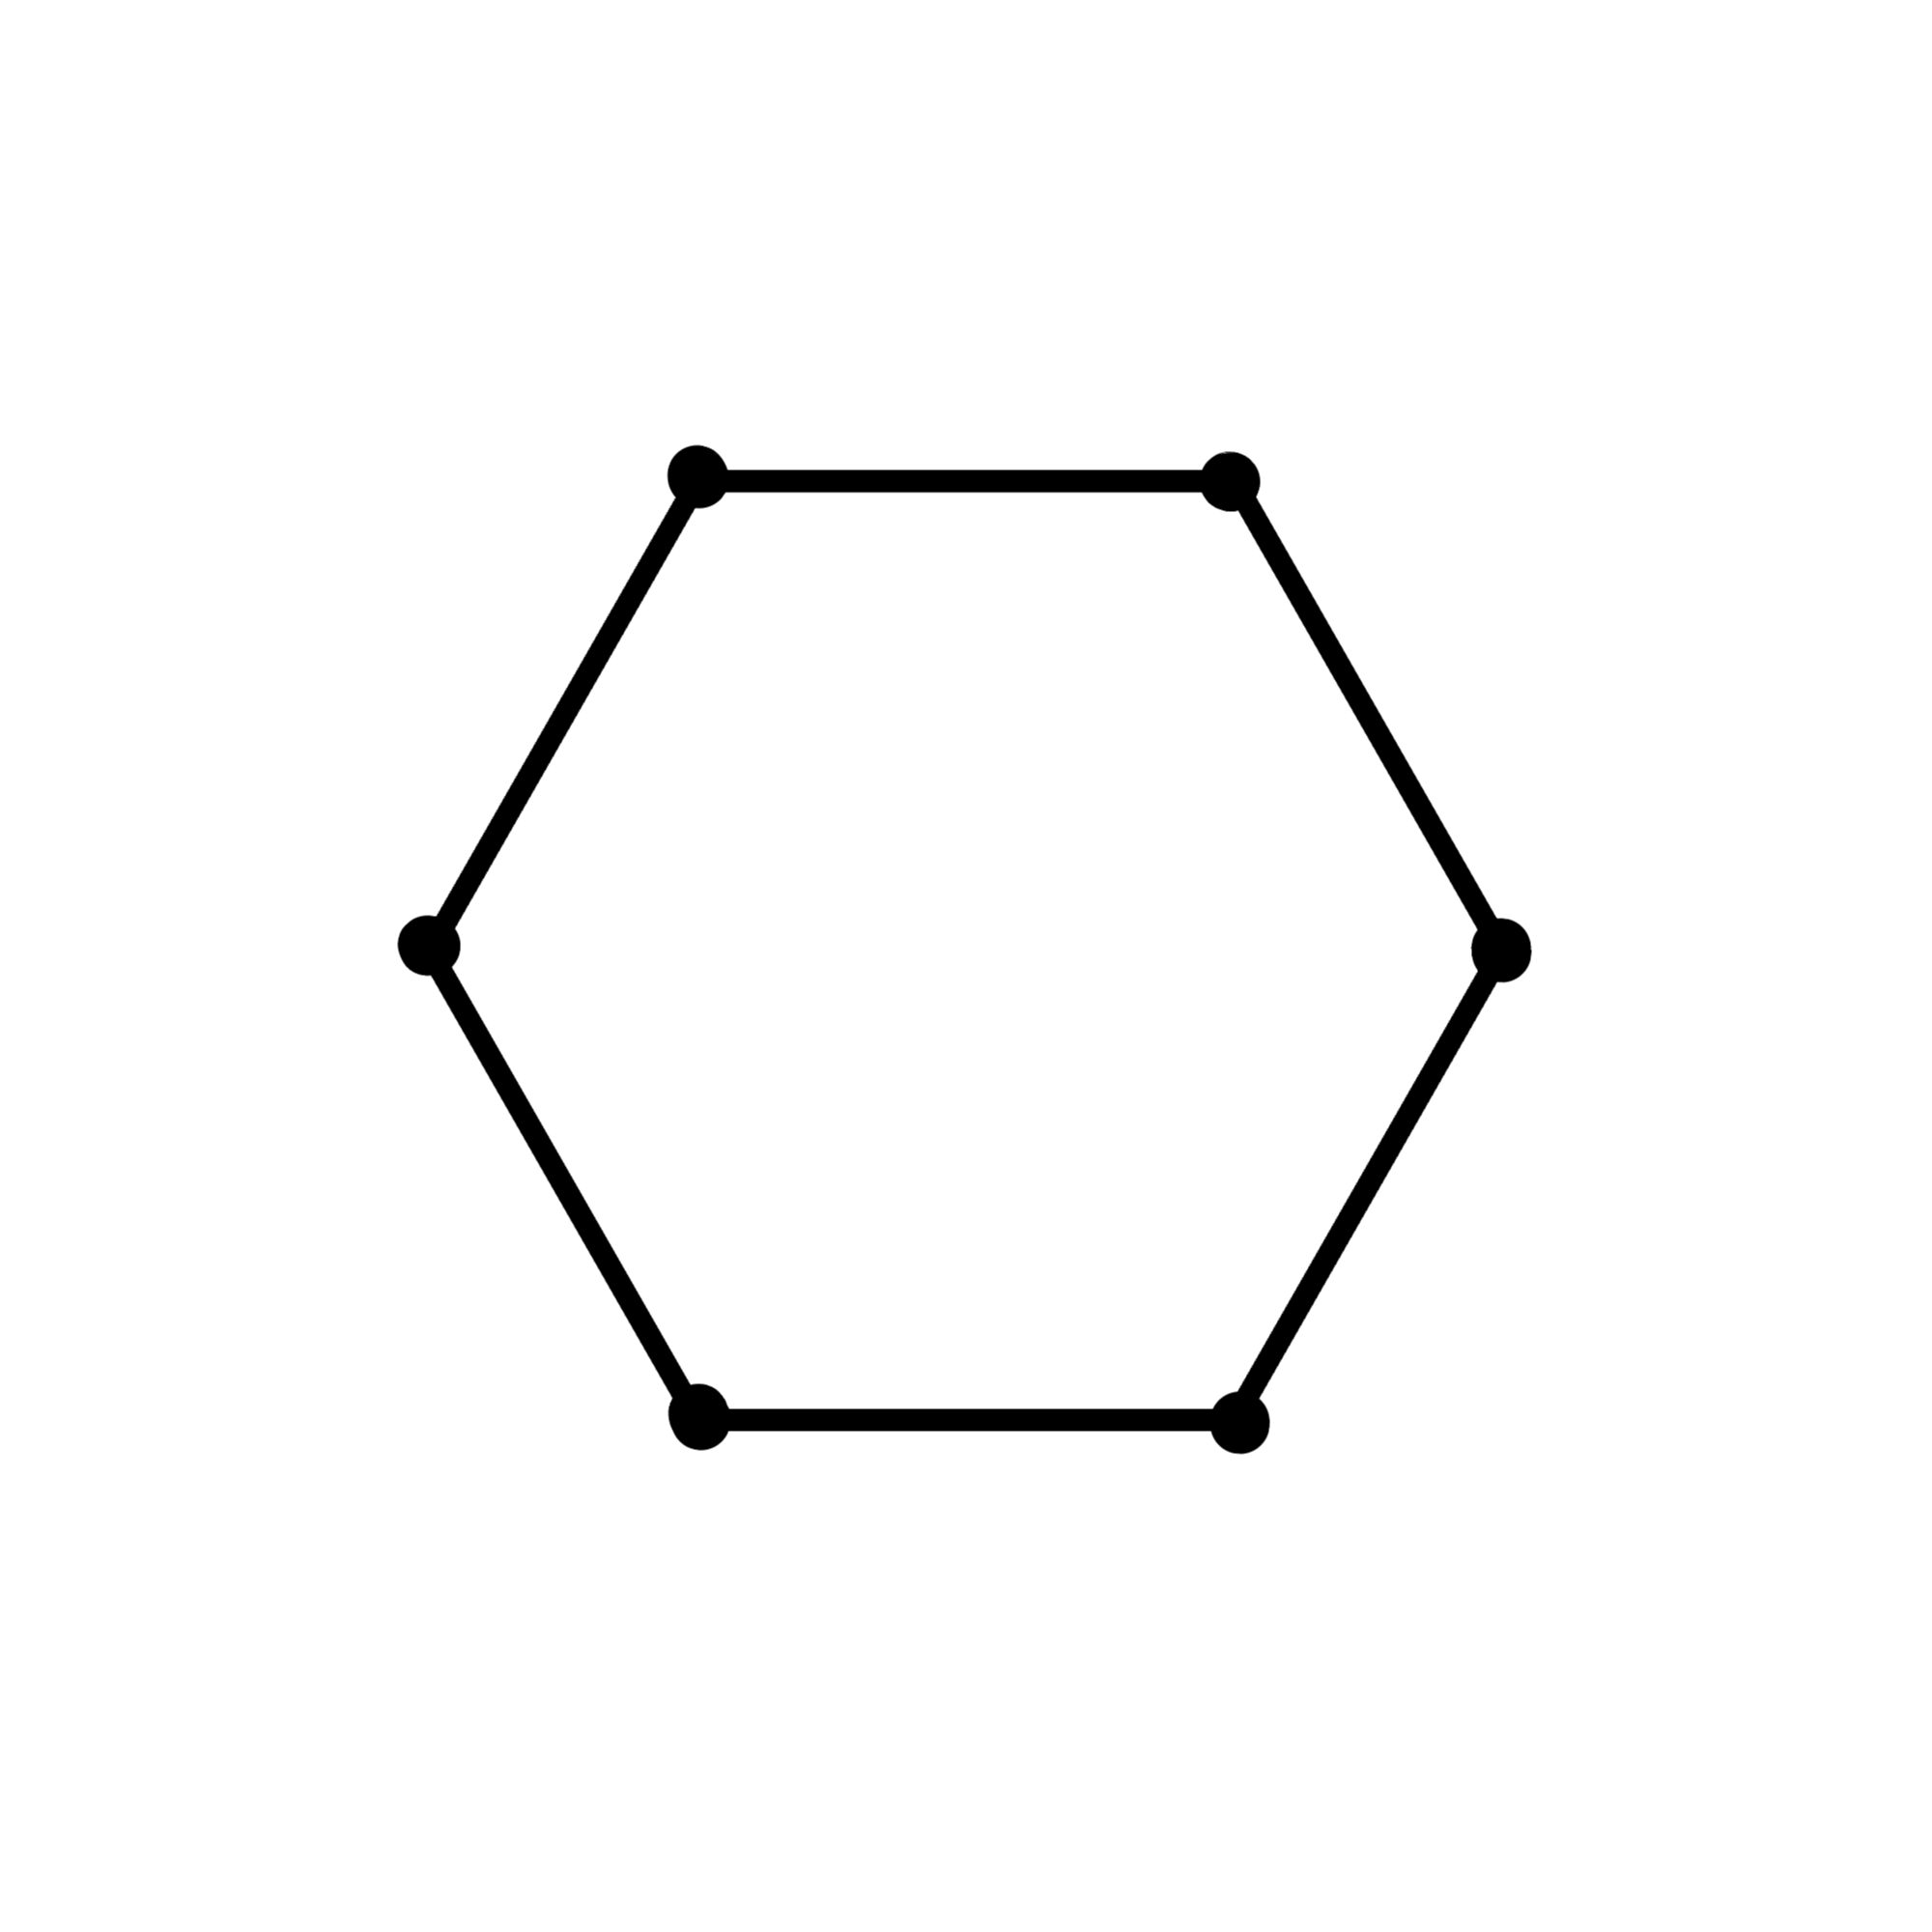
\includegraphics[width=4cm]{gfx/Cayley graph D6 sq.png}}} % [ ]: \vspace*{-2cm} 
    \subfloat[\centering \(\Delta (3,3,3)\)]{{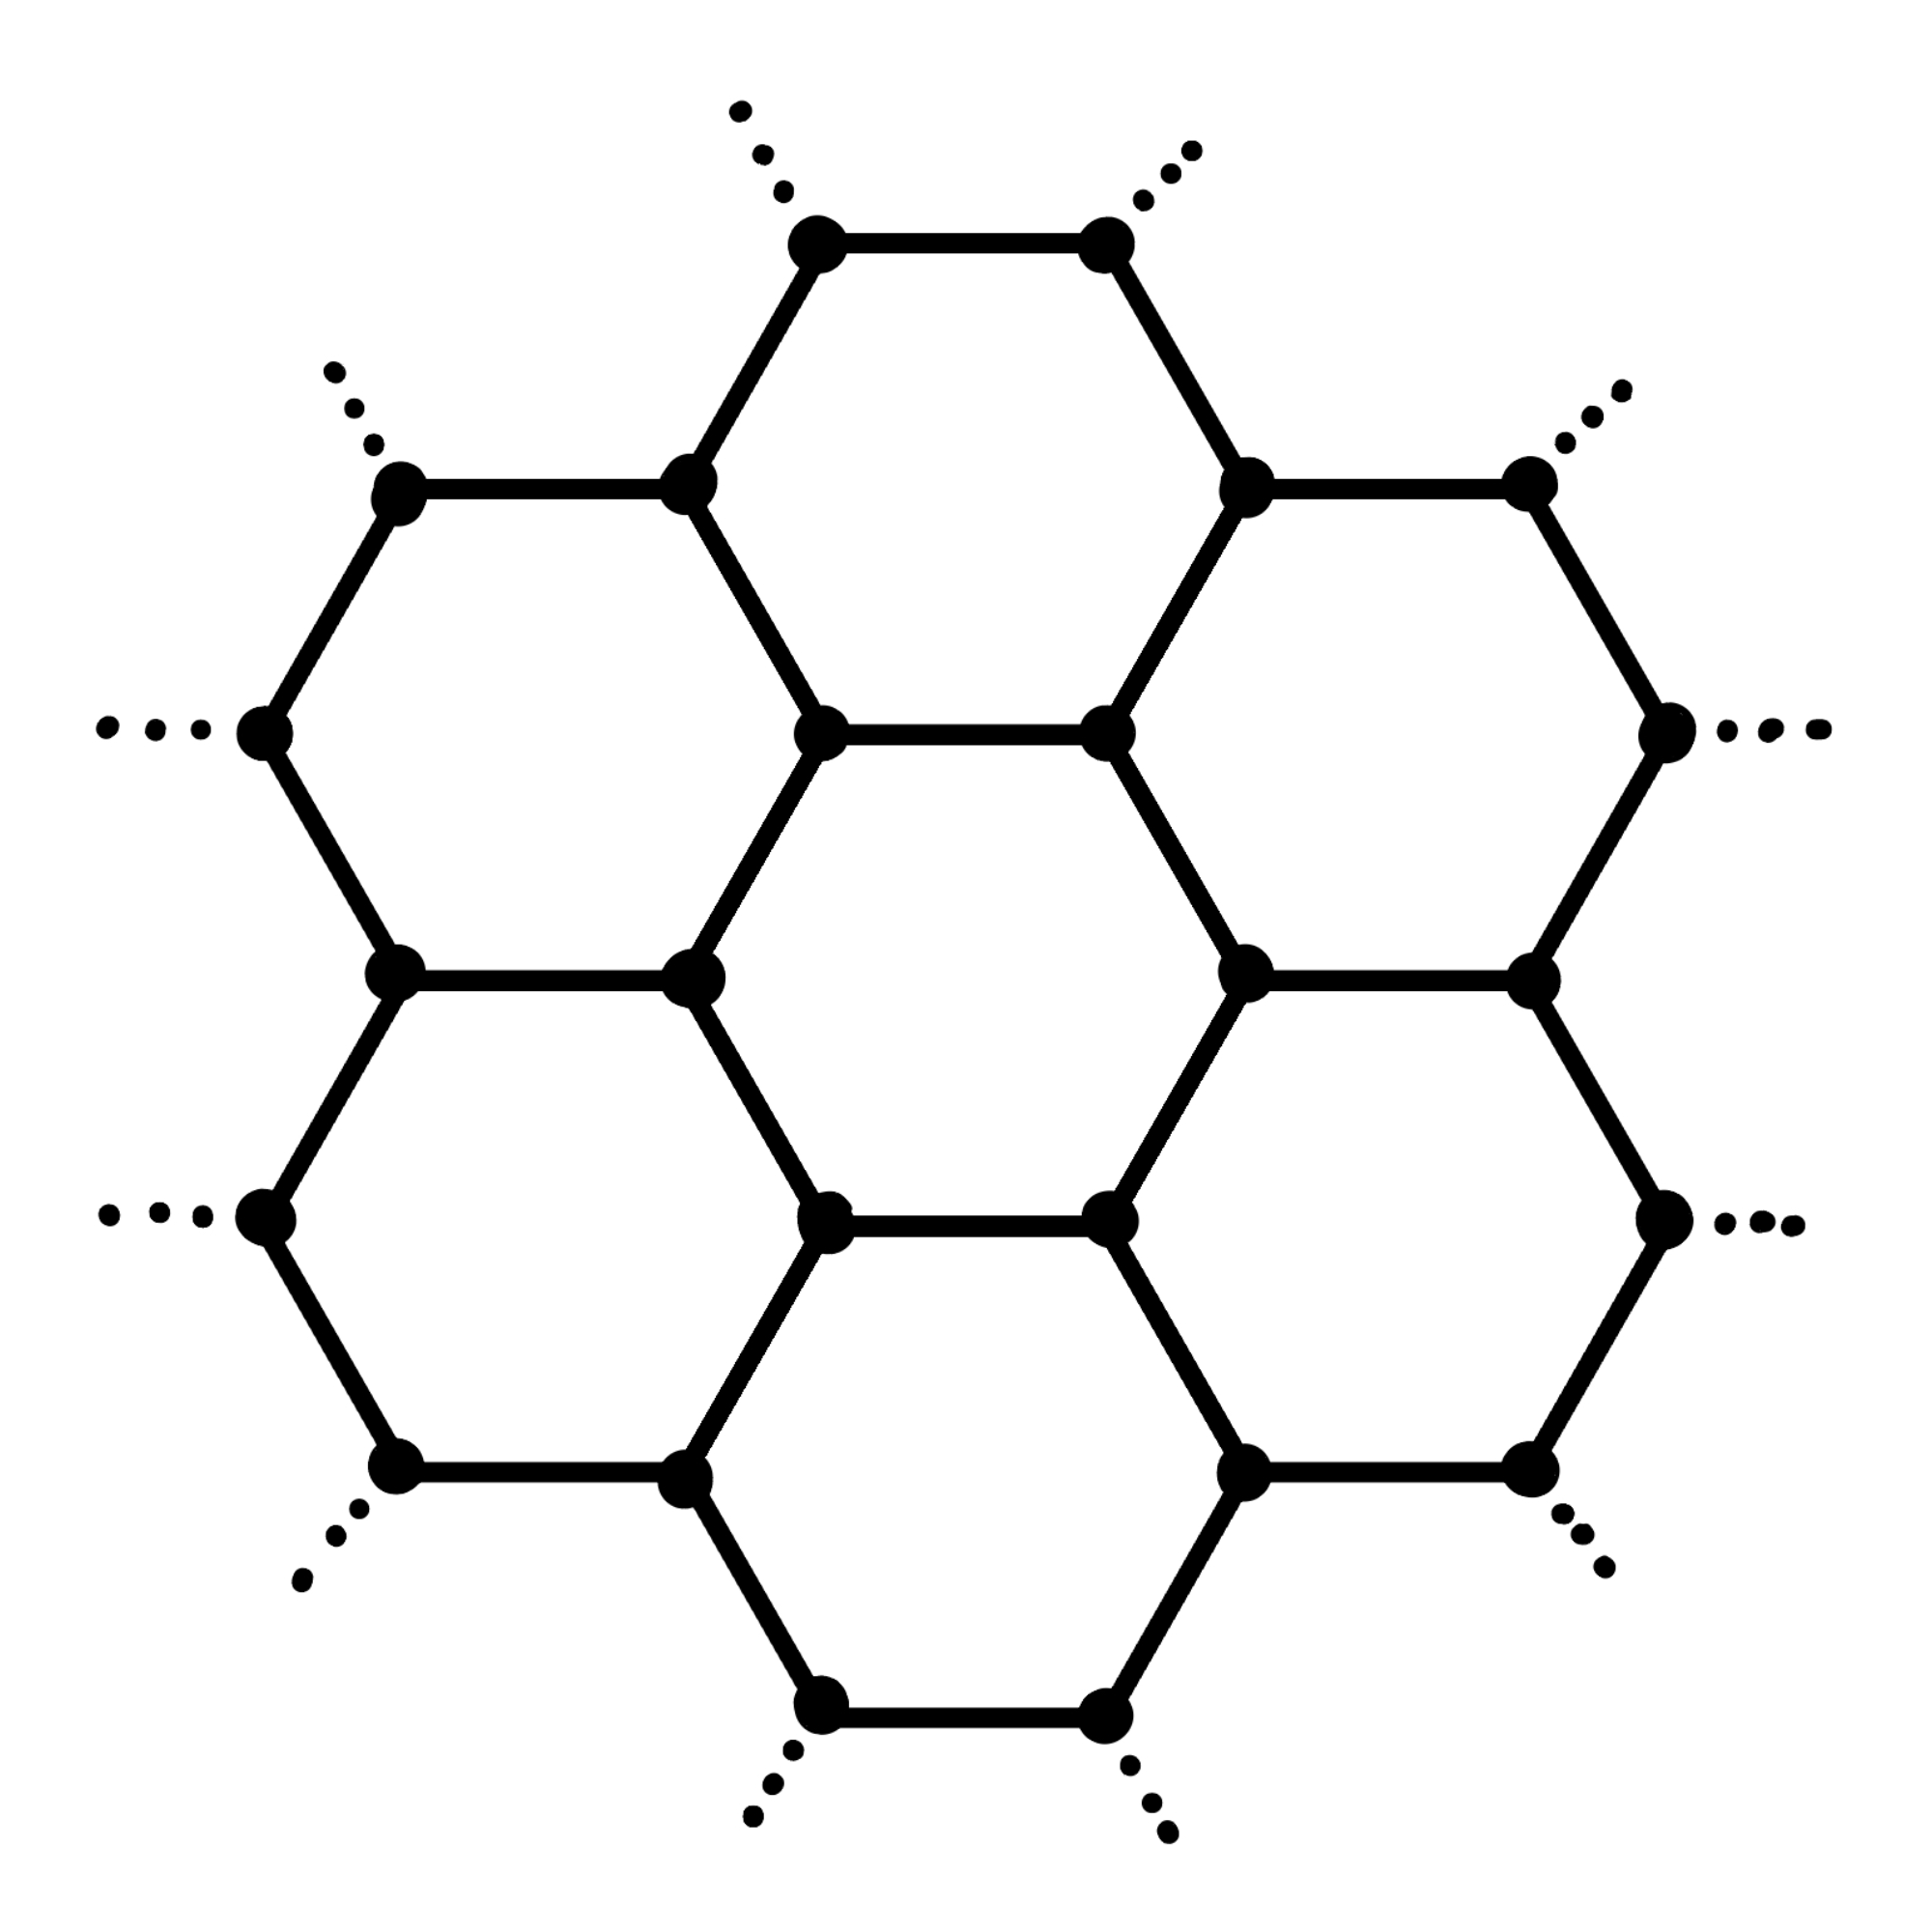
\includegraphics[width=4cm]{gfx/Cayley graph triangle group sq.png}}}
    \subfloat[\centering \(D_\infty\)]{{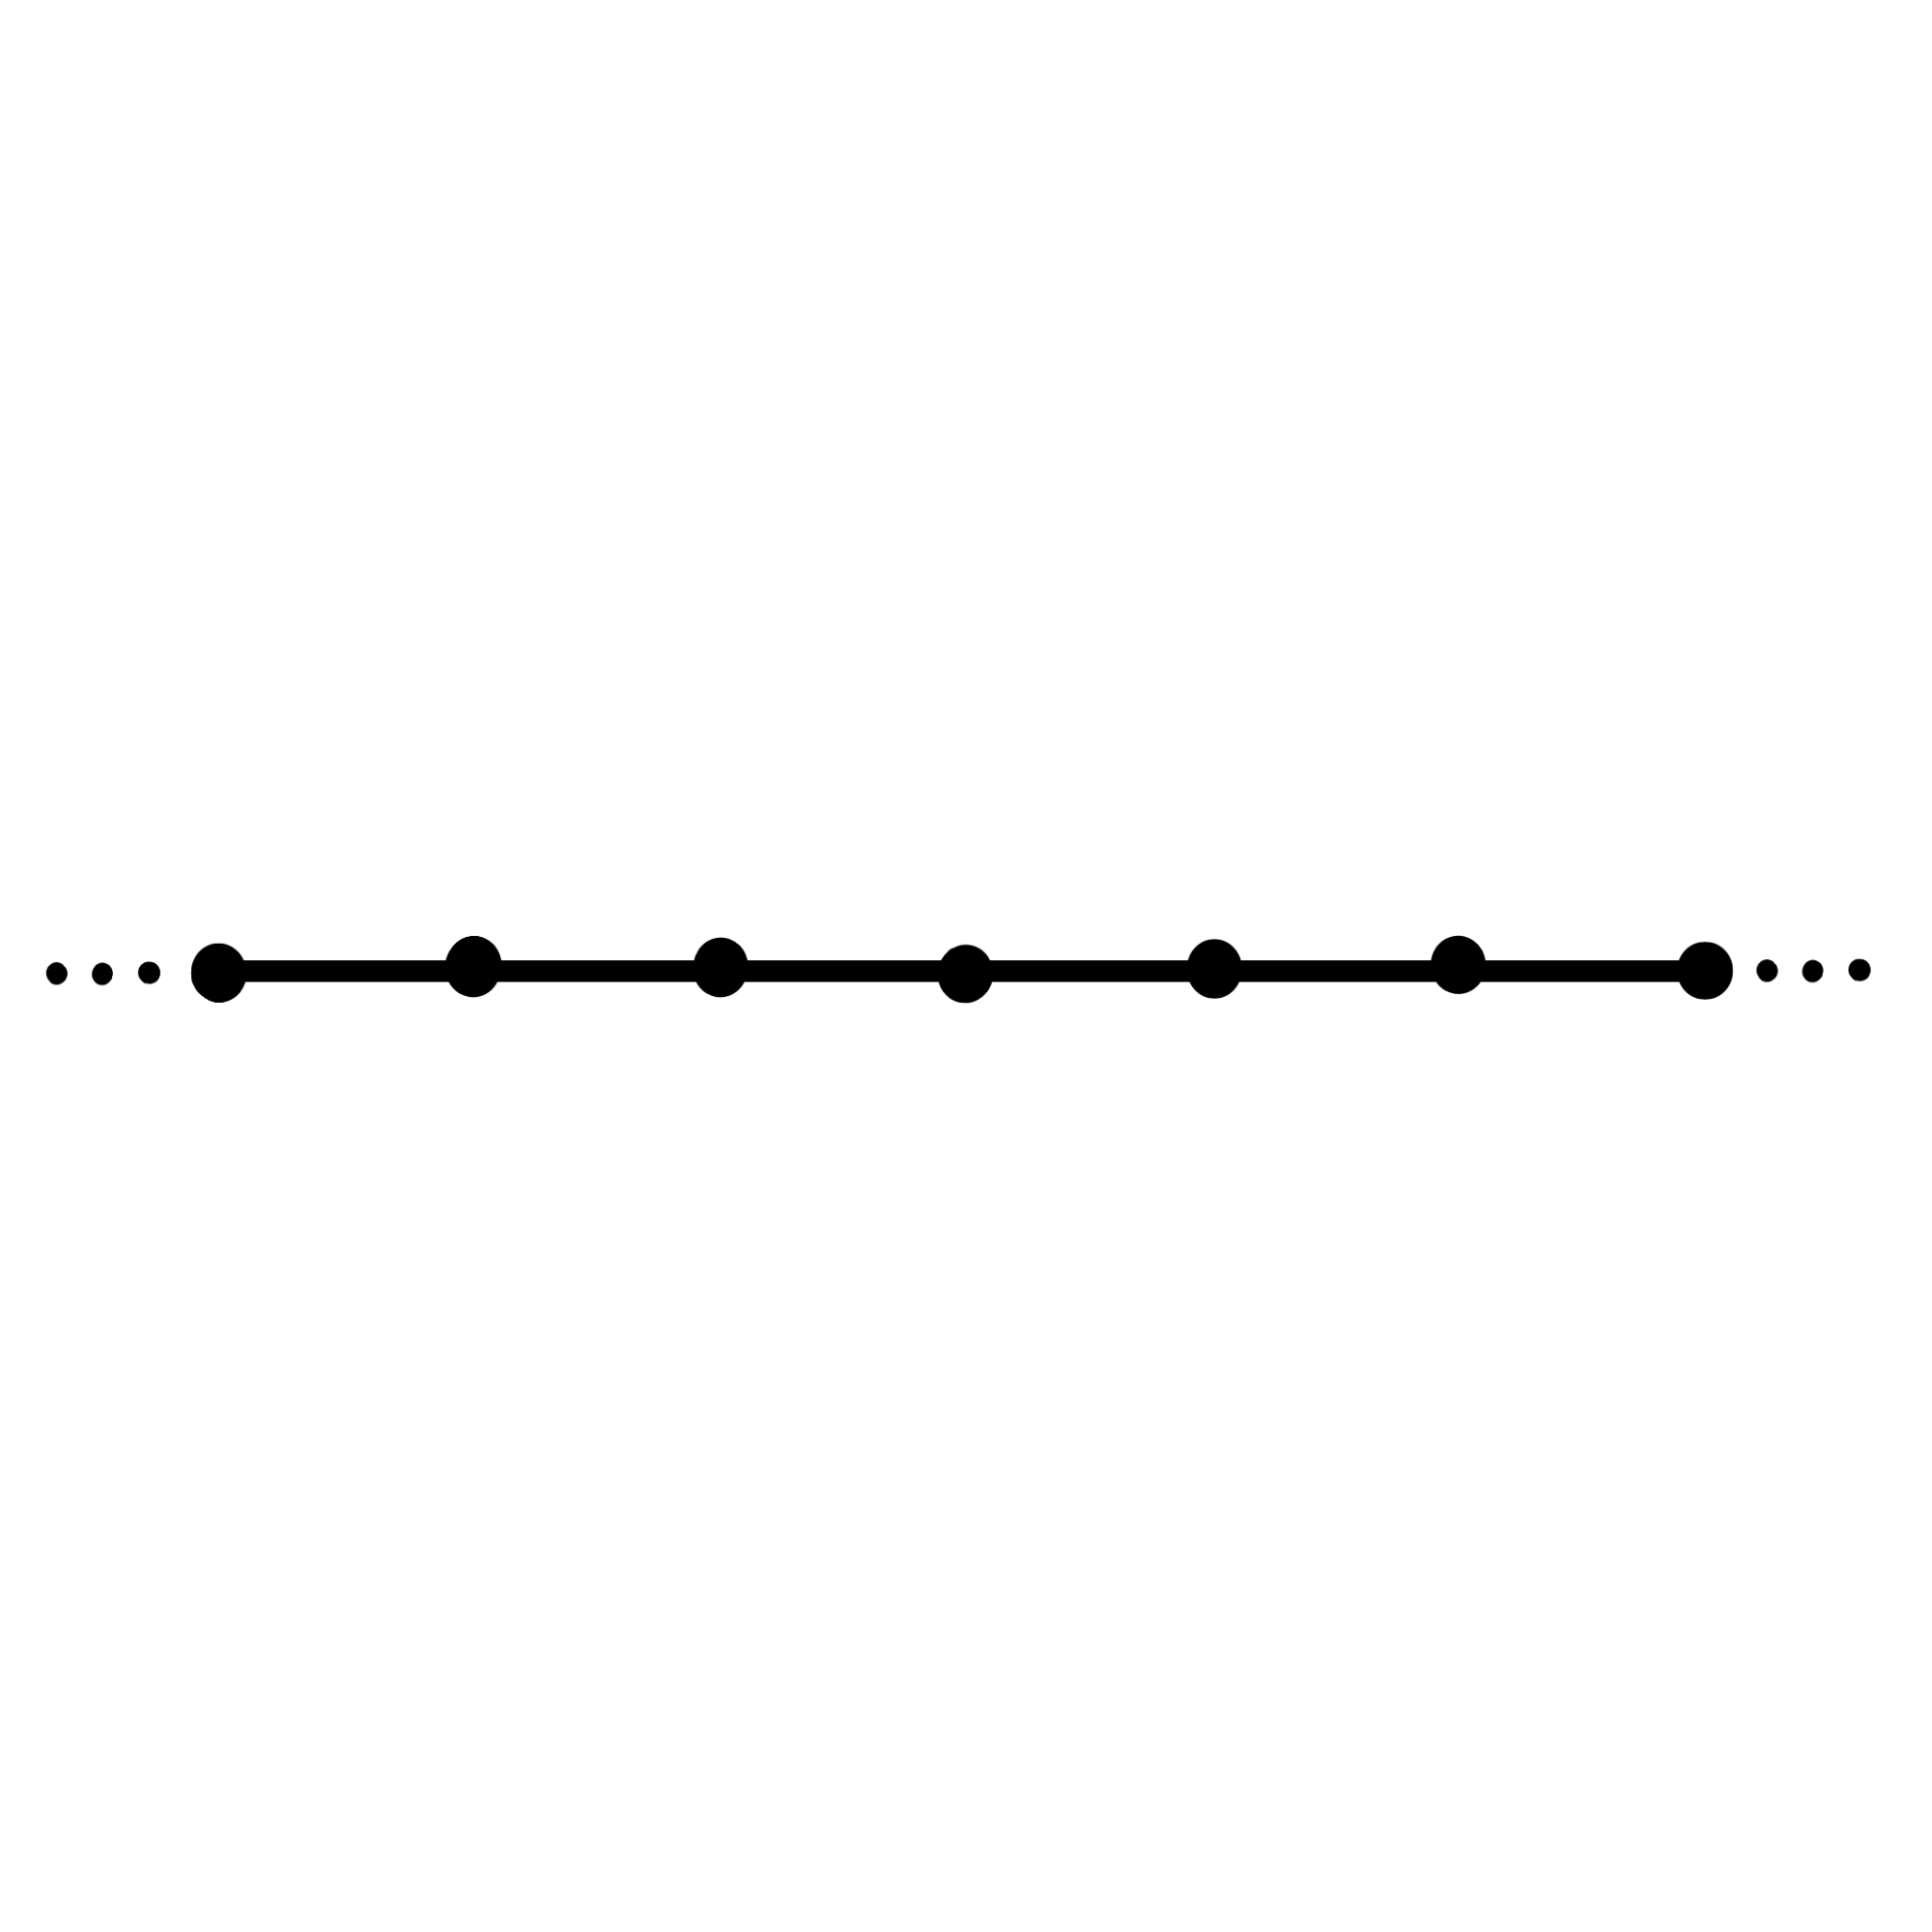
\includegraphics[width=4cm]{gfx/Cayley graph Dinfty sq.png}}}
    \subfloat[\centering \(\faktor{\Z}{2\Z}\ast\faktor{\Z}{2\Z}\ast\faktor{\Z}{2\Z}\)]{{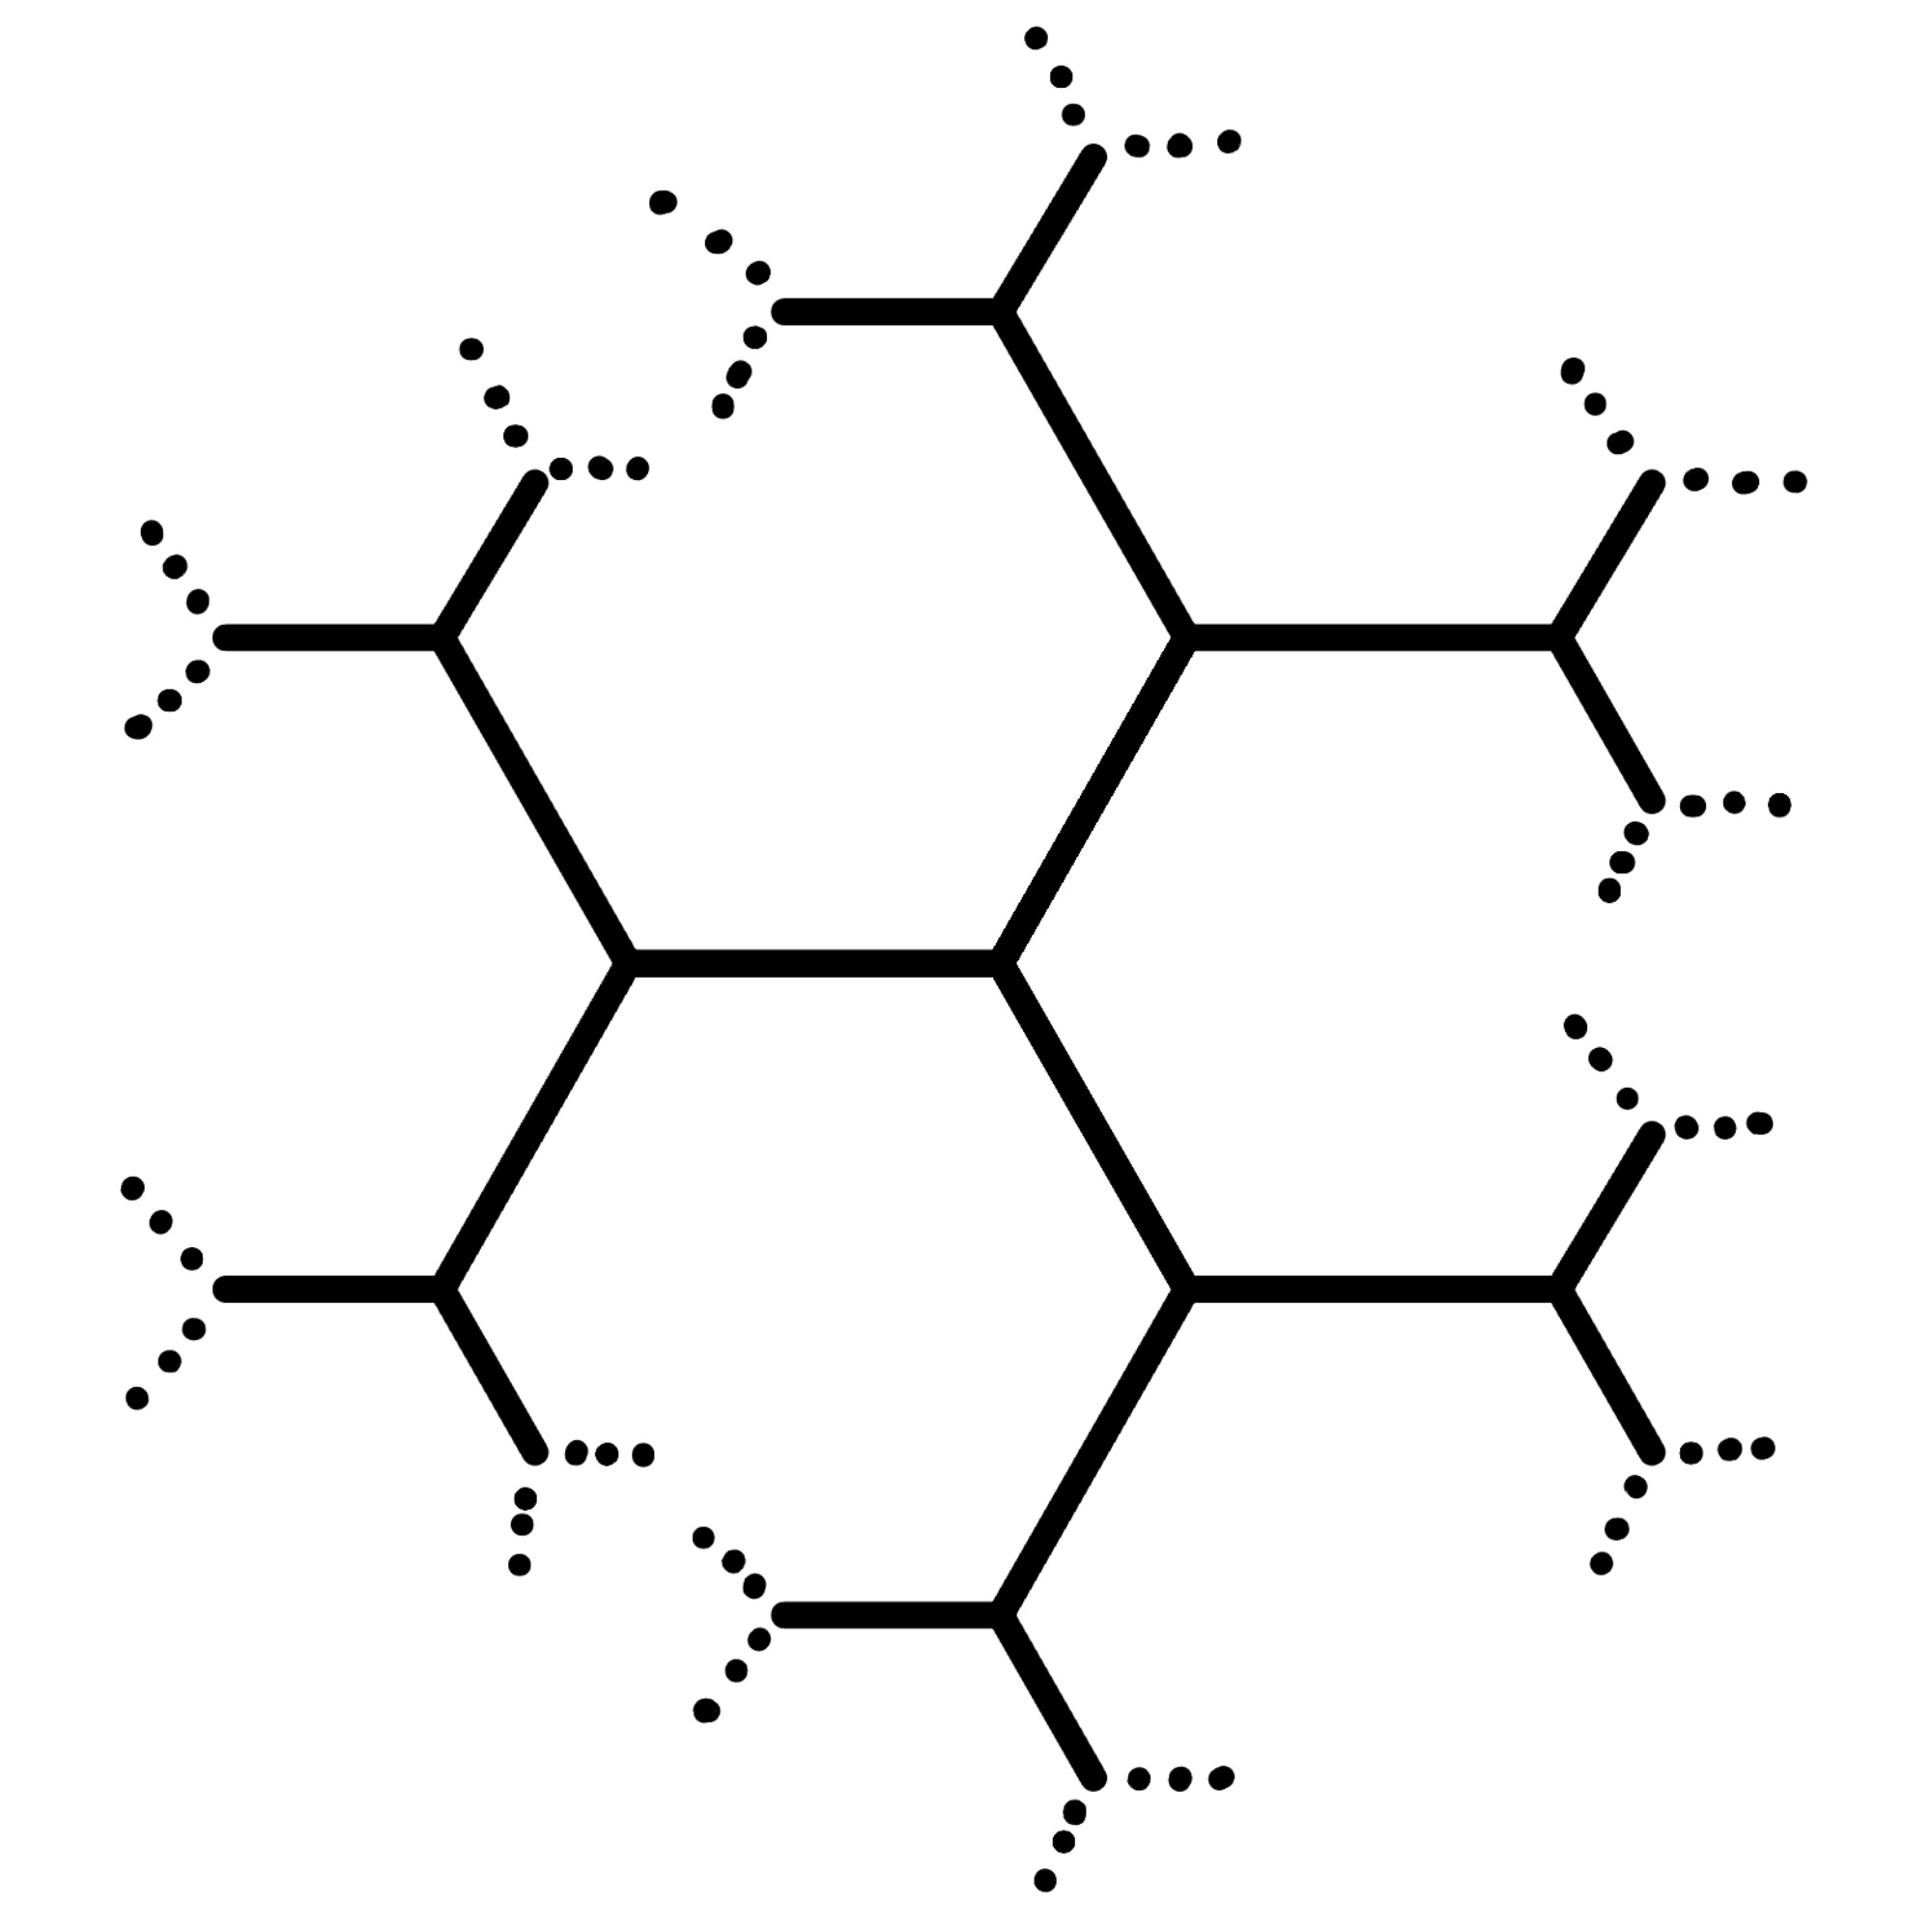
\includegraphics[width=4cm]{gfx/Cayley graph free product sq.png}}}
\end{figure}

We define a special type of subgroups, called parabolic subgroups within a Coxeter group \(W\).
These subgroups are constructed from a subset of the index set \(I\).
The definition is as follows:

\begin{definition}
    Let \((W,S)\) be a Coxeter System as above with finite index set \(I\), and \(J\) be a subset of the index set \(I\).
    The group \(W_J := \langle\{s_j \;\vert\; j\in J\}\rangle\), generated by the \(s_j\) in \(S\) with \(j \in J\), is then called a \emph{parabolic subgroup} of \(W\).
    Moreover, we call any conjugate of \(W_J\) a parabolic subgroup as well.
\end{definition}

Once we have constructed the representation of Coxeter groups on a vector space as well as the Tits cone in the coming section, the parabolic subgroups will be a useful tool to form a deeper understanding of these objects.
We will extensively use them in Sections \(2.4\) and \(2.5\).

% ***********************************************
\section{Representation of Coxeter groups}
% ***********************************************

Given a Coxeter System \((W,S)\), let \(V\) be a real vector space with basis \(\{e_1,\ldots,e_n\}\), where \(n=\abs{I}=\abs{S}\).
This provides a natural identification, \(GL_n(V)\cong GL_n(\R)\).
We define a bilinear form \(B_W\) on \(V\) as follows:
\begin{equation*}
    B_W(e_i, e_j) := \begin{cases}
        -\cos \left(\frac{\pi}{m_{ij}}\right) & ,\; m_{ij}<\infty \\
        -1                                    & ,\; m_{ij}=\infty
    \end{cases}.
\end{equation*}
By \Cref{def:CoxeterGroup}, it is assured that \(m_{ij}\geq 2\) for distinct \(i,j\), ensuring the cosine term is non-positive.
Consequently, we have \(B_W(e_i,e_j)\leq 0\) for distinct \(i,j\).
Furthermore, from \(m_{ii}=1\), it follows that \(B_W(e_i,e_i)=1\).
Using this bilinear form, we define hyperplanes with corresponding reflections for each basis element \(e_i\) as follows:
\[H_i := \{v\in V\;\vert\; B_W(e_i,v) = 0\}\;, \qquad \sigma_i : V\to V,\quad v\mapsto v - 2B_W(e_i,v)e_i.\]

\begin{theorem}\label{thm:repr}
    The map given by:
    \[\rho : W \to GL_n(V) \cong GL_n(\R), \quad s_i \mapsto \sigma_i\]
    is an injective homomorphism and therefore a faithful representation of \(W\).
\end{theorem}
Before we prove the homomorphism property, we recall:
A map \(\varphi: S\to G\) from a set \(S\) to a group \(G\) extends to a homomorphism \(\Hat{\varphi}:\groupp{S}{R}\to G\), if and only if the induced homomorphism \(\overline{\varphi}:F_S \to G\) from the free group over \(S\) satisfies \(\overline{\varphi}(r) = 1_G\) for every \(r\in R\).
\begin{proof}
    Observe that \(\sigma_i^2 = id\) in \(GL_n(V)\) and thus to prove that \(\rho\) is a homomorphism, we apply the above to our situation to see that it suffices to show that the product \(\sigma_i\sigma_j\) has order \(m_{ij}\) in \(GL_n(V)\) for distinct \(i,j\in I\).
    Also note that in the case of \(m_{ij} = \infty\) there is nothing to prove as these relations are defined to be trivial in the presentation of \(W\).
    
    Thus, consider the two-dimensional subspace \(V_{ij}\) of \(V\) spanned by two basis vectors \(e_i, e_j\) and take a general element \(v = \lambda \cdot e_i + \mu \cdot e_j\) in \(V_{ij}\) with \(\lambda, \mu \in \R\) not simultaneously zero.
    As \(m_{ij} < \infty\), the bilinear form \(B_W\) is positive definite by the following calculation
    \[B_W (v,v) = \lambda^2 - 2\lambda\mu\cos\left(\frac{\pi}{m_{ij}}\right) + \mu^2 = \left(\lambda - \mu \cos\left(\frac{\pi}{m_{ij}}\right)\right)^2 + \mu^2\sin^2\left(\frac{\pi}{m_{ij}}\right) > 0.\]
    Identify \((V_{ij}, B_W\vert_{V_{ij}})\) with the euclidean plane \((\R^2, \langle \cdot, \cdot \rangle)\) up to a change of basis.
    Then \(\sigma_i\), resp. \(\sigma_j\) act by orthogonal reflections in their corresponding hyperplanes \(H_i\), resp. \(H_j\) intersected with \(V_{ij}\).
    By having a look at the inner product of \(e_i\) and \(e_j\)
    \[B_W(e_i, e_j) = - \cos\left(\frac{\pi}{m_{ij}}\right) = \cos\left(\pi - \frac{\pi}{m_{ij}}\right),\]
    we observe that the angle between the two in \(V_{ij}\) is precisely \(\pi - \frac{\pi}{m_{ij}}\).
    We conclude from this that the angle between their reflecting lines in \(\frac{\pi}{m_{ij}}\) and the composition \(\sigma_i\sigma_j\) turns out to be a rotation about \(\frac{2\pi}{m_{ij}}\).
    As the composition \(\sigma_i\sigma_j\) fixes the orthogonal complement \(V_{ij}^\perp\) of \(V_{ij}\) by definition of the \(\sigma_i\), we see that it has order \(m_{ij}\) on the whole space \(V\).
    % To do so, consider the two-dimensional subspace \(V_{ij}\) spanned by two basis vectors \(e_i\) and \(e_j\) in \(V\).
    % We take a general element \(v = \lambda e_i + \mu e_j\), \(\lambda,\mu\in\R\) in \(V_{ij}\) and distinguish the two cases in the definition of \(B_W\):
    % \begin{itemize}
    %     \item[1)] \(m_{ij}<\infty\): In this case \(B_W\) is positive definite, since for \(v\neq 0\)
    %           \begin{align*}
    %               B_W(v,v) & = \lambda^2 - 2\lambda\mu\cos\left(\frac{\pi}{m_{ij}}\right) + \mu^2
    %               = \left( \lambda - \mu\cos\left( \frac{\pi}{m_{ij}} \right) \right)^2 + \mu^2\sin^2\left( \frac{\pi}{m_{ij}} \right) > 0.
    %           \end{align*}
    %           Up to a change of basis, we identify \((V_{ij}, B_W\vert_{V_{ij}})\) with the euclidean plane \((\R^2, \langle\cdot, \cdot\rangle)\).
    %           Now \(\sigma_i\) and \(\sigma_j\) act on \(V_{ij}\) by orthogonal reflections in the hyperplanes \(H_i, H_j\) intersected with \(V_{ij}\).
    %           We take a look at the inner product of \(e_i, e_j\)
    %           \[B_W(e_i, e_j) = -\cos\left(\frac{\pi}{m_{ij}}\right) = \cos\left(\pi - \frac{\pi}{m_{ij}}\right)\]
    %           and obtain that the angle between them in \(V_{ij}\) is given by \(\pi - \frac{\pi}{m_{ij}}\).
    %           Thus, the angle between the reflecting lines is \(\frac{\pi}{m_{ij}}\) and the product \(\sigma_i\sigma_j\) turns out to be a rotation by \(\frac{2\pi}{m_{ij}}\), showing that \(\sigma_i\sigma_j\) has order \(m_{ij}\) in the subspace \(V_{ij}\).
    %           And since \(\sigma_i\sigma_j\) fixes the orthogonal complement of \(V_{ij}\) by definition of the \(\sigma_i\), it has order \(m_{ij}\) on the whole vector space \(V\).

    %     \item[2)] \(m_{ij} = \infty:\;\) By the following, we now have to deal with a non-positive definite form:
    %           \begin{align*}
    %               B_W(v,v) = \lambda^2 - 2\lambda\mu + \mu^2 = (\lambda - \mu)^2 \geq 0.
    %           \end{align*}
    %           Indeed, we can only expect it to be positive semidefinite on \(V_{ij}\).
    %           Using the calculation
    %           \begin{align*}
    %               (\sigma_i\sigma_j)(e_i) = \sigma_i (e_i + 2e_j) = e_i + 2(e_i + e_j),
    %           \end{align*}
    %           together with an induction argument, we get that \((\sigma_i\sigma_j)^n(e_i) = e_i + 2n(e_i + e_j)\).
    %           Therefore, the concatenation has infinite order on \(V_{ij}\) and in particular on the whole of \(V\).
    % \end{itemize}
    This proves that \(\rho\) extends to a homomorphism.
    It remains to show the injectivity of \(\rho\).
    This will be a consequence of a bigger result in section \(2.4\), see \Cref{cor:faithful}.
\end{proof}

In contrast to the above proof, in the case of \(m_{ij} = \infty\), we cannot expect our bilinear form to be positive definite.
Let \(v \in V_{ij}\) be as in the proof, then
\[B_W(v,v) = \lambda^2 - 2\lambda\mu + \mu^2 = (\lambda - \mu)^2 \geq 0.\]
This shows that we can at least expect it to be positive semidefinite.
The direct calculation
\[(\sigma_i\sigma_j)(e_i) = \sigma_i(e_i + 2e_j) = e_i + 2(e_i + e_j),\]
together with an inductive argument, shows that \((\sigma_i\sigma_j)^n(e_i) = e_i + 2n(e_i + e_j)\).
Therefore, the composition \(\sigma_i\sigma_j\) has infinite order on \(V_{ij}\) and in particular on the whole of \(V\).
The following remark is a consequence of this, together with the observation in above proof.

\begin{remark}
    From last paragraph and the proof of \Cref{thm:repr}, we conclude that two-generator subgroups of Coxeter groups are dihedral.
    Either of order \(2m_{ij}\) or infinite order.
\end{remark}

We want to extend the action of \(W\) to the dual of the vector space \(V\).
This is achieved by acting on \(V^*\) via the dual representation of \(\rho\), which we define by
\[\rho^* : W \to GL_n(V^*),\quad w \mapsto (\rho^*(w): V^* \to V^*, \; \varphi \mapsto \rho^*(w)(\varphi)), \quad w\in W, \varphi\in V^*.\]
We can evaluate the functional \(\rho^*(w)(\varphi)\) on some \(v \in V\) via \((\rho^*(w)(\varphi))(v) := \varphi(\rho(w^{-1})(v))\).
Notation wise, we will simply write \(w(v)\), when \(w \in W\) acts on \(v \in V\) via \(\rho(w)(v)\).
Similarly, we write \(w(\varphi)\) when we mean that \(w \in W\) acts on some element \(\varphi \in V^*\) of the dual space, via the dual representation \(\rho^*(w)(\varphi)\).
As in the case of the vector space \(V\), we want to give a definition for the notion of a hyperplane with corresponding reflection in the dual space \(V^*\) as well.
By dual hyperplane, we mean a subspace \(H_i^* := \{\varphi \in V^* \;\vert\; \varphi (e_i) = 0\}\), and the corresponding dual reflections will be a map from \(V^*\) to \(V^*\), given by:
\[\sigma_i^* : V^* \to V^*,\quad \varphi \mapsto \varphi \circ \sigma_i = \varphi - 2B_W(e_i,\;\cdot\;)\varphi(e_i).\]

To further explore Coxeter groups and their action via this representation, we need some more notation.
In particular, we want a so-called \emph{chamber}.
This should be thought of as a cone over a polytope with finitely many faces such that the reflections in its codimension one faces correspond to the generators of \(W\) under the representation.

\begin{definition}\label{def:chamber}
    The fundamental chamber \(C\) of the dual representation is the set, given by
    \[C := \{\varphi \in V^* \;\vert\; \varphi (e_i) \geq 0 \;\forall i\in I\} \subset V^*.\]
\end{definition}

Denote by \(\{e_1^*,\ldots, e_n^*\}\) the dual basis of \(V^*\) corresponding to the standard basis \(\{e_1,\ldots, e_n\}\) of \(V\).
Then we calculate, using the \(\sigma_i^*\) from above:
\begin{equation*}
    \sigma_i^*(e_j^*) = e_j^* - 2B_W(e_i,\cdot)e_j^*(e_i) =
    \begin{cases}
        e_j^*                   & \text{for } i\neq j \\
        e_j^* - 2B_W(e_j,\cdot) & \text{for } i=j
    \end{cases},
\end{equation*}
which implies that each reflection \(\sigma_i^*\) fixes all the hyperplanes \(H_j^*\), for distinct indices \(i\) and \(j\).
Moreover, note that the fundamental chamber can be written in the form % TODO: rework the following paragraph --
\[C = \bigcap_{i\in I}\{\varphi\in V^*\;\vert\; \varphi(e_i)\geq 0\} = \bigcap_{i\in I} (H_i^* \cup \{\varphi\in V^*\;\vert\; \varphi(e_i)> 0\}),\]
where we observe that the sets \(H_i^*\cap C\) form the pairwise distinct codimension one faces of the chamber \(C\).
The open halfspaces \(\{\varphi \in V^* \;\vert\; \varphi(e_i) > 0\}\) in the latter term will be called \(A_i^*\) and using these, we define the open fundamental chamber to be the intersection of the open halfspaces:
\[\text{int}(C) = \mathring{C} = \bigcap_{i \in I} A_i^*.\] % ---------
As mentioned above, we want to study the action of our Coxeter group via the dual representation, acting by reflection in the faces \(H_i^*\).
However, in general the translates of the chamber under the group action won't cover the whole of \(V^*\), which motivates the following definition:

\begin{definition}
    The Tits cone is the union of all \(W\)-translates of the chamber, \(WC := \underset{w \in W}{\bigcup} wC \subset V^*\).
\end{definition}

As the name suggests, the fundamental chamber is a fundamental domain for the action of \(W\) on its Tits cone \(WC\) under the dual representation \(\rho^*\).
This will be proved in \Cref{thm:funddomain}.
While the formal defintion of the Tits cone provides a rigorous foundation, it is not very insightful from a geometric perspective.
As one can think about the Tits cone quite geometrically, especially in low dimensions, we will take a closer look at an explicit example in the following section.
Before doing so, we end this section with the following remark.

\begin{remark} % TODO: add picture
    One may ask why we transport everything to the dual space, instead of working in the standard representation \(\rho\).
    For this, consider the infinite dihedral group \(D_\infty \cong \groupp{s, t}{s^2 = t^2 = 1}\).
    We fix a basis \(\{e_1, e_2\}\) of \(V\) and obtain that the bilinear form in this basis is given by the matrix
    \begin{equation*}
        B_W = \begin{pmatrix}
            1  & -1 \\
            -1 & 1
        \end{pmatrix}.
    \end{equation*}
    We observe that \(H_1 = \text{span}\{e_1 + e_2\} = H_2\), which implies that \(\sigma_1\) and \(\sigma_2\) fix the same hyperplane, despite having different \((-1)\)-Eigenspaces (namely the span of \(e_1\), resp. \(e_2\)).
    Therefore, in general, working in the standard representation won't result in a chamber, giving rise to the existence of the Tits cone.
    Now, passing to the dual space \(V^*\) by fixing the dual basis \(\{e_1^*, e_2^*\}\), consider the dual reflections \(\sigma_i^*\) as discussed before.
    By the more general calculation earlier, we obtain
    \[\sigma_1^*(H_2^*) = H_2^* \quad\text{and}\quad \sigma_2^*(H_1^*) = H_1^*.\]
    And furthermore, we note that for all \(i,j\in\{1,2\}\)
    \[\sigma_i^*(B_W(e_j,\cdot)) = B_W(e_j,\cdot) - 2B_W(e_i,\cdot)B_W(e_j,e_i) = - B_W(e_j,\cdot),\]
    using that \(B_W(e_j,\cdot) = -B_W(e_i,\cdot)\).
    This shows that both dual reflections have the same \((-1)\)-Eigenspace, but fix different hyperplanes (\ie, have different \((+1)\)-Eigenspaces), resulting in a chamber as wished.
\end{remark}

% \begin{figure}[h!]
%     \label{fig:firstchamber}
%     \centering
%     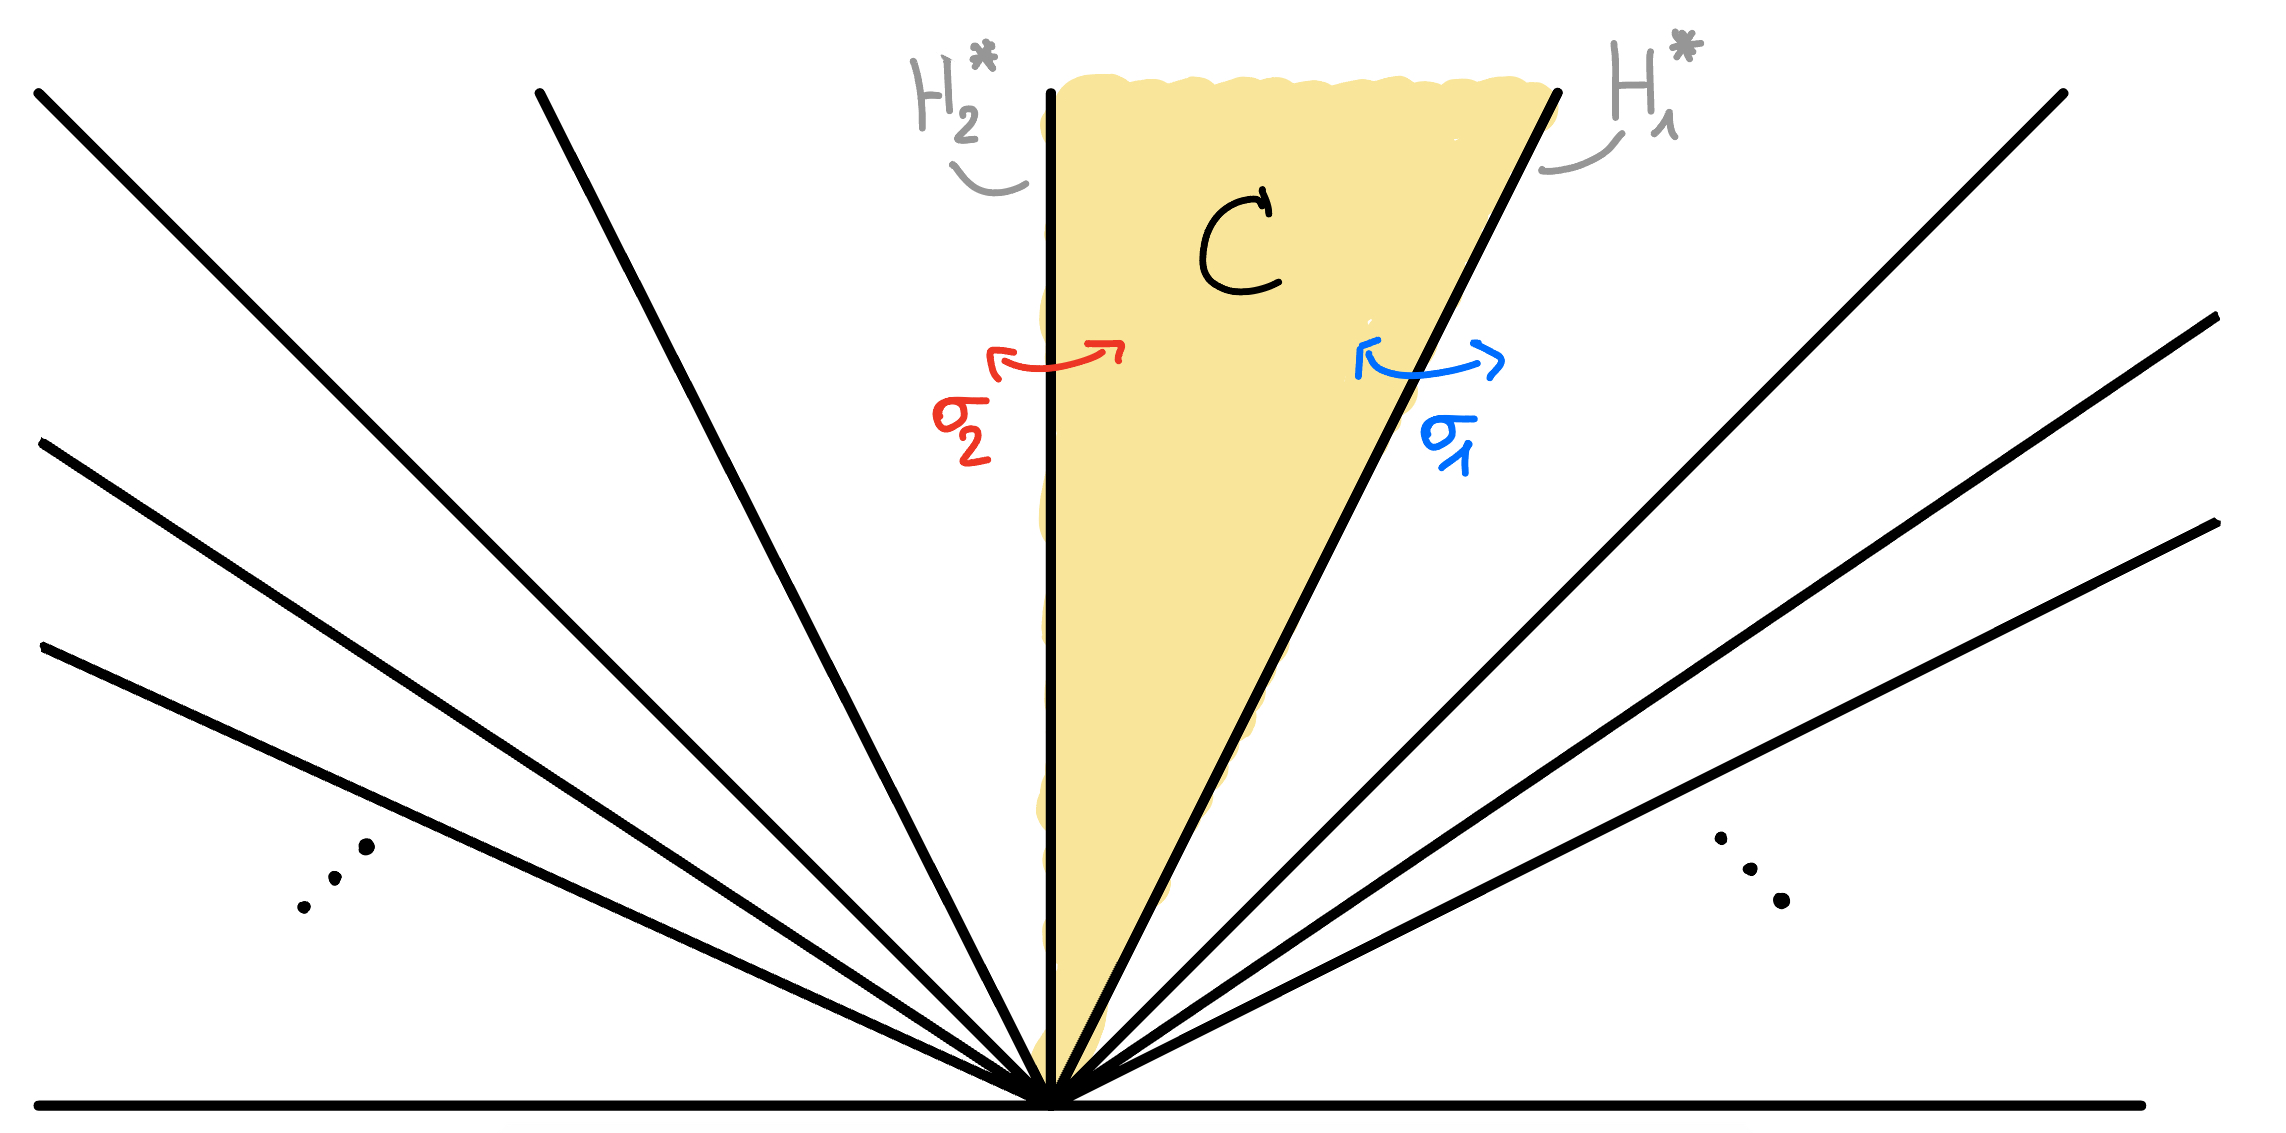
\includegraphics[width=.75\textwidth]{gfx/Chamber of Dinfty.png}
%     \caption{The chamber of \(D_\infty\)}
% \end{figure}


% ***********************************************
\section{The Tits cone - An example} % TODO: add picture
% ***********************************************

As an example we take a closer look at the free product \(W \cong\groupp{r,s,t}{r^2=s^2=t^2=1}\), a right-angled Coxeter group from \Cref{ex:freeprod}.
We fix the basis \(\{e_1,e_2,e_3\}\) and identify \(V\) with \(\R^3\).
In this basis, the bilinear form \(B_W\) is given by the matrix
\begin{equation*}
    B_W =
    \begin{pmatrix}
        1  & -1 & -1 \\
        -1 & 1  & -1 \\
        -1 & -1 & 1
    \end{pmatrix}.
\end{equation*}
By the spectral theorem we find a basis of orthonormal Eigenvectors, in which \(B_W\) is a diagonal matrix with its eigenvalues as entries.
Using the Gram-Schmidt procedure, we get
\begin{equation*}
    \begin{pmatrix}
        -\frac{1}{\sqrt{2}} & 0                  & \frac{1}{\sqrt{2}}  \\
        -\frac{1}{\sqrt{6}} & \frac{2}{\sqrt{6}} & -\frac{1}{\sqrt{6}} \\
        \frac{1}{\sqrt{3}}  & \frac{1}{\sqrt{3}} & \frac{1}{\sqrt{3}}
    \end{pmatrix} \cdot
    \begin{pmatrix}
        1  & -1 & -1 \\
        -1 & 1  & -1 \\
        -1 & -1 & 1
    \end{pmatrix} \cdot
    \begin{pmatrix}
        -\frac{1}{\sqrt{2}} & -\frac{1}{\sqrt{6}} & \frac{1}{\sqrt{3}} \\
        0                   & \frac{2}{\sqrt{6}}  & \frac{1}{\sqrt{3}} \\
        \frac{1}{\sqrt{2}}  & -\frac{1}{\sqrt{6}} & \frac{1}{\sqrt{3}}
    \end{pmatrix} =
    \begin{pmatrix}
        2 & 0 & 0  \\
        0 & 2 & 0  \\
        0 & 0 & -1
    \end{pmatrix}.
\end{equation*}
In other words, we have \(V^T B_W V = D\) with \(V\in O(n)\) and \(D = \text{diag}(2,2,-1)\).
Now, since we have a diagonal matrix, we can multiply the entries by squares, since the resulting matrix will be congruent to the given one:

Let \(A = \text{diag}(\mu_1,\ldots,\mu_n)\in\R^{n\times n}\),
\begin{equation*}
    S=\text{diag}(\lambda_1,\ldots, \lambda_n)\in(\R\setminus\{0\})^{n\times n} \implies S^TAS = \text{diag}(\lambda_1^2\mu_1,\ldots,\lambda_n^2\mu_n).
\end{equation*}
To apply this and further transform our matrix \(D\), define the invertible matrix \(T\) as follows
\[T = \begin{pmatrix} \frac{1}{\sqrt{2}} & 0 & 0 \\ 0 & \frac{1}{\sqrt{2}} & 0 \\ 0 & 0 & 1 \end{pmatrix},\]
which then implies \(\widetilde{D} := T(V^T B_W V)T = \text{diag}(1,1,-1)\).
The images of the basis vectors \(\{e_1,e_2,e_3\}\) are given by the three columns of the matrix \(TV^T\), namely:
\begin{equation*}
    \widetilde{e}_1 = \begin{pmatrix} -\frac{1}{2} \\ - \frac{\sqrt{3}}{6} \\ \frac{1}{\sqrt{3}} \end{pmatrix},\;
    \widetilde{e}_2 = \begin{pmatrix} 0 \\ \frac{1}{\sqrt{3}} \\ \frac{1}{\sqrt{3}} \end{pmatrix} \text{ and }
    \widetilde{e}_3 = \begin{pmatrix} \frac{1}{2} \\ -\frac{\sqrt{3}}{6} \\ \frac{1}{\sqrt{3}} \end{pmatrix}.
\end{equation*}
Note that we have \(V\cong \R^3\), equipped with the inner product
\[\langle x, y \rangle_{2,1} := x^T\widetilde{D}y = x_1y_1 + x_2y_2 - x_3y_3.\]
Since \(\langle \widetilde{e}_i, \widetilde{e}_i \rangle_{2,1} = 0\) for all \(i\in \{1,2,3\}\), we have that these three vectors span an ideal triangle in the hyperboloid model of \(\HH^2\), given by \(\langle x, y \rangle_{2,1} = -1\).
One gets the ideal triangle by intersecting the hyperboloid with the hyperplanes spanned by each two of the \(\widetilde{e}_i\) (they will only intersect in the surrounding cone of the hyperboloid).

Given these new coordinates under the transformation \(TV^T\), the Tits cone will be given by \(x_1^2 + x_2^2 - x_3^2 < 0\) union the images of \(\widetilde{e}_1, \widetilde{e}_2\) and \(\widetilde{e}_3\) under the reflection in the sides of the chamber, i.e. in the sides of the ideal triangle. % TODO: under the transformation TV^t
Moreover, we get a subgroup of \(O(2,1)_+\) generated by the following three matrices
\begin{equation*}
    \begin{pmatrix} 1 & 0 & 0 \\ 0 & -\frac{5}{3} & -\frac{4}{3} \\ 0 & \frac{4}{3} & \frac{5}{3} \end{pmatrix},\;
    \begin{pmatrix} -1 & \frac{2}{\sqrt{3}} & -\frac{2}{\sqrt{3}} \\ \frac{2}{\sqrt{3}} & \frac{1}{3} & \frac{2}{3} \\ \frac{2}{\sqrt{3}} & -\frac{2}{3} & \frac{5}{3} \end{pmatrix}
    \text{ and }
    \begin{pmatrix} -1 & -\frac{2}{\sqrt{3}} & \frac{2}{\sqrt{3}} \\ -\frac{2}{\sqrt{3}} & \frac{1}{3} & \frac{2}{3} \\ -\frac{2}{\sqrt{3}} & -\frac{2}{3} & \frac{5}{3} \end{pmatrix}.
\end{equation*}
Each of the above matrices corresponds to one of the generators \(r, s\) and \(t\) of the right angled Coxeter group \(W\) under the transformation \(TV^T\), constructed above.

\begin{figure}[h!]
    \label{fig:titsconeex}
    \centering
    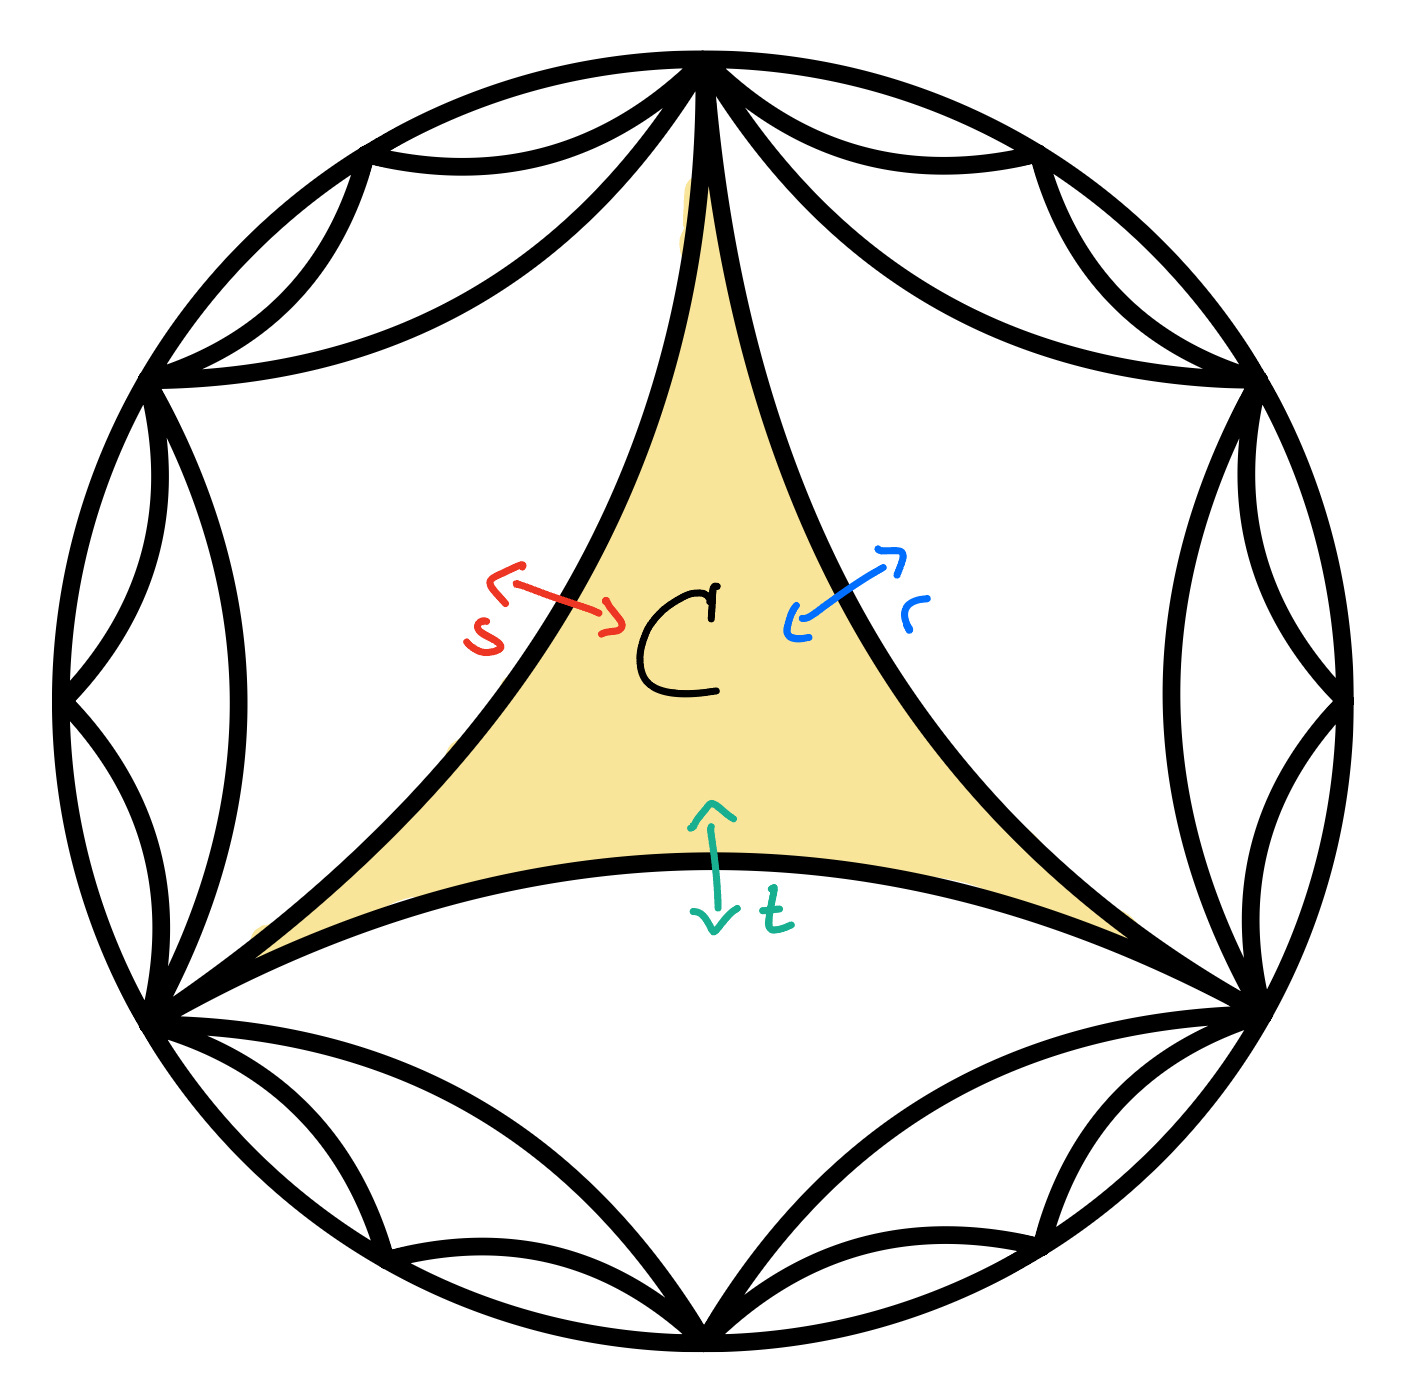
\includegraphics[width=5cm]{gfx/Tits cone example poincare.png}
    \caption{The Tits cone in the poincaré disc.}
\end{figure}

% ***********************************************
\section{The word metric and the faithful representation}
% ***********************************************

Recall that for any finitely generated group \(W = \langle S \rangle\), its Cayley graph induces a metric on \(W\), relative to the generating set \(S\).
We call it the \emph{word metric} of \(W\) relative to \(S\) and denote it by \(d_S\).
Also note that the word metric is left-invariant, meaning that for group elements \(u,v,w\in W\), we have the equality \(d_S(uv,uw) = d_S(v,w)\).
Now, define the \emph{word length} of an element \(w\in W\) to be \(\ell(w) := d_S(w, 1_W)\), the distance of an element to the neutral element of the group.
Note that \(\ell(w) = 0\) if and only if \(w = 1_W\).

\begin{lemma}
    We collect some properties of the length function we will use later on.
    \begin{enumerate}
        \item \(\forall w\in W:\; \ell(w) = \ell(w^{-1})\)
        \item \(\forall s\in S:\; \ell(s) = 1\) and \(\ell(w) = 1 \iff w\in S^{\pm 1}\)
        \item \(\forall v,w\in W:\; \ell(vw)\leq\ell(v)+\ell(w)\)
        \item \(\forall v,w\in W:\; \ell(v)-\ell(w)\leq\ell(vw)\)
        \item \(\forall w\in W, s\in S^{\pm 1}:\; \ell(w)-1\leq\ell(ws)\leq\ell(w)+1\)
    \end{enumerate}
\end{lemma}
\begin{proof}
    All of the above statements follow from the fact that \(d_S\) is a left-invariant metric.
    % \begin{enumerate}
    %     \item For \(w\in W\), write the length of w as \(\ell(w) = d_S(w, e_W)\).
    %           By the left-invariance of \(d_S\), we have \(d_S(w, e_W) = d_S(e_W, w^{-1})\) and by symmetry of \(d_S\), \(\ell(w) = \ell(w^{-1})\) follows.
    %     \item This is true by definition.
    %     \item For \(u,v\in W\), using the triangle inequality of \(d_S\), we get: \[\ell(uv) = d_S(uv, e_W) \leq d_S(u, e_W) + d_S(v, e_W) = \ell(u) + \ell(w).\]
    %     \item For \(v,w\in W\) we have \(\ell(v)=\ell(vww^{-1})\leq\ell(vw) + \ell(w^{-1})\), by point 3 and thus, using point 1: \(\ell(v) - \ell(w) \leq \ell(vw)\).
    %     \item For \(w\in W,\; s\in S\), apply point 3 and point 4 to \(\ell(ws)\).
    % \end{enumerate}
\end{proof}

Coming back to Coxeter groups, by definition each generator \(s\in S\) has order 2 in \(W\).
Therefore, we can write every non-trivial element in \(W\) as a sequence of generators in \(S\).
Note that in this sequence there might be redundencies, so that the following definition makes sense.
We call an expression \(w = s_{i_1} \cdots s_{i_r}\) for \(i_1,\ldots, i_r\in I\) and \(r\in\N\) \emph{reduced}, if \(\ell(w) = r\), \ie \(\;w\) cannot be represented by a shorter word.
These reduced expressions have the caveat of not being unique by any means.

Given a parabolic subgroup \(W_J\) of a Coxeter group \(W\), it admits its own word metric with respect to \(J\subset I\).
Therefore each parabolic subgroup admits its own length function, which we denote by \(\ell_J(w)\) for words \(w\) in \(W_J\).
In the following we will make use of the general fact that we have \(\ell(w) \leq \ell_J(w)\) for all \(w\in W_J\).

The length function turns out to be an important and powerful tool in studying Coxeter groups.
Indeed, its role will be demonstrated in several of the forthcoming proofs, beginning with the following theorem which is a key step in proving faithfulness of our previously defined representation.
But before doing so, we want to motivate the next theorem. % [ ]: nötig?
We consider the set \(\{w(e_i) \;\vert\; i \in I, w \in W\}\).
Note that we fixed a basis in our representation vector space and therefore each of these elements can be written as a linear combination of the basis vectors.
We will use this to define `positive' and `negative' elements.
An element \(w(e_i)\) is said to be
\begin{itemize}
    \item positive (denoted \(w(e_j) > 0\)), if \(w(e_j) = \sum_{i \in I} \lambda_i e_i\) with \(\lambda_i \geq 0\) for all \(i \in I\),
    \item negative (denoted \(w(e_j) < 0\)), if \(w(e_j) = \sum_{i \in I} \lambda_i e_i\) with \(\lambda_i \leq 0\) for all \(i \in I\).
\end{itemize}

\begin{theorem}\label{thm:action}
    Let \(w\in W\) and \(s_i\in S\) for \(i\in I\).
    Then \(\ell(ws_i) > \ell(w)\) implies that \(w(e_i) > 0\).
\end{theorem}

% The proof is by induction on the word length \(\ell(w)\).
% To apply the induction hypothesis, the central idea is to decompose \(w\) in a suitable way.

\begin{proof}
    The base case is trivial, as \(\ell(w) = 0\) implies \(w = 1_W\) and thus \(w\) fixes every basis element.
    Therefore, assume \(w\) is non-trivial and in reduced form.
    We state the induction hypothesis.
    \IH{Let \(v \in W\), so that \(\ell(v) < \ell(w)\) and \(\ell(vs_i) > \ell(v)\), then we have \(v(e_i) > 0\).}
    \Claim{1}{There is a \(j\in I\) such that \(s_i\neq s_j\) and \(\ell(ws_j) = \ell(w) - 1\).}
    \Claimproof{1}{
        Since \(w\) is in reduced form, write \(w = s_{i_1}\cdots s_{i_k}\) and set \(s_j = s_{i_k}\).
        This implies \[\ell(ws_i) > \ell(w) > \ell(w) - 1 = \ell(ws_j),\]
        and in particular \(s_j\neq s_i\).
        This proves the first Claim.
    }
    Consider the parabolic subgroup \(\langle s_i, s_j\rangle\leq W\), generated by these two distinct elements in \(S\).
    % Denote this subgroup by \(W_J\), for \(J=\{i,j\}\subset I\).
    Set \(J := \{i, j\}\) in \(I\) and denote the subgroup by \(W_J\).
    We use the decomposition \(W = W/W_J \cdot W_J\) to decompose \(w\) into two parts, each living in one component.
    % Our goal now is to decompose \(w\) into two parts, one living in the subgroup \(W_J\) and the other in its complement.
    For this, consider a specific subset of the coset \(wW_J\), given by % coset representatives
    \[A:=\{v\in W \;\vert\; vW_J = wW_J \;\text{ and }\; \ell(v) + \ell_J(v^{-1}w) = \ell(w)\}.\]
    By definition, \(w\in A\).
    With regard to the following, we choose \(v\in A\) such that its length \(\ell(v)\) is minimal.
    % Note that since \(vW_J = wW_J\), we have that \(W_J = v^{-1}wW_J\), implying that \(v^{-1}w\in W_J\).
    % In view of the comment above, set \(v_J = v^{-1}w \iff w = vv_J\), decomposing \(w\) as desired.
    Now set \(v_J = v^{-1}w\), which is equivalent to writing \(w = vv_J\), giving us a decomposition of \(w\) as desired.
    Due to this decomposition, our analysis of \(w\) now boils down to studying the separate actions of \(v\) and \(v_J\) on \(V\).
    First note that \(ws_j\) is contained in \(A\) as well.
    Clearly, \(s_j^{-1} = s_j\) and thus we have that
    \[s_jw^{-1}w = s_j\in W_J \text{ and } \ell(ws_j) + \ell_J(s_j) = \ell(w) - 1 + 1 = \ell(w).\]
    By the choice of \(\ell(v)\) to be minimal, we have \(\ell(v)\leq \ell(ws_j) = \ell(w)-1\), implying \(\ell(v) < \ell(w)\).
    Hence, we are almost set up to apply the induction hypothesis to \(v\) and \(s_i\).
    The last ingredient missing to do so is the following Claim.
    \Claim{2}{For the lengths of \(vs_i\) and \(v\), we have the relation: \(\ell(vs_i) \geq \ell(v)\).}
    \Claimproof{2}{
        Assume towards contradiction: \(\ell(vs_i) < \ell(v)\), equivalently \(\ell(vs_i) = \ell(v) - 1\).
        Then:
        \begin{align*}
            \ell(w) & = \ell(vv_J) = \ell(vs_is_iv^{-1}w) \leq \ell(vs_i) + \ell(s_iv^{-1}w)        \\
                    & \leq \ell(v) - 1 + \ell_J(v^{-1}w) + 1 = \ell(v) + \ell_J(v^{-1}w) = \ell(w).
        \end{align*}
        This means equality holds throughout and in particular \(\ell(w) = \ell(vs_i) + \ell_J(s_iv^{-1}w)\).
        But this implies \(vs_i\) belongs to \(A\), contradicting the minimality of \(\ell(v)\).
        Thus, the claim holds.
    }
    Applying the induction hypothesis \textbf{(IH)} to \(v\) and \(s_i\) leaves us with \(v(e_i) > 0\).
    The exact same argument applied to \(v\) and \(s_j\) shows \(v(e_j) > 0\), so that we omit this here.
    % Thus, we are now reduced to the rank two situation, where we observe how \(v_J\) acts on \(e_i\).
    % First of all, we have
    Due to the decomposition and the fact that \(w\) lies in \(W_J\), we are now reduced to the rank two situation.
    As we have seen that all two generator subgroups are dihedral, we work in the flat plane.
    But first, we have to observe the following claim.
    \Claim{3}{For \(v_Js_i\) and \(v_J\), we have the relation: \(\ell_J(v_Js_i)\geq \ell(v)\).}
    \Claimproof{3}{
        Assume towards contradiction, that \(\ell_J(v_Js_i) < \ell(v_J)\) holds. Then:
        \begin{align*}
            \ell(ws_i) = \ell(vv_Js_i) \leq \ell(v) + \ell(v_Js_i) \leq \ell(v) + \ell_J(v_Js_i) < \ell(v) + \ell_J(v_J) = \ell(w),
        \end{align*}
        which contradicts the assumption of the theorem, that \(\ell(ws_i) > \ell(w)\).
    }
    Moreover, this shows that every reduced expression of \(v_J\) in the parabolic subgroup \(W_J\) has to end in \(s_j\).
    Otherwise, we would have \(\ell(v_J) > \ell(v_J s_i)\), which contradicts \emph{Claim 3}.
    To deduce the theorem, it suffices to show the following claim.
    % \Claim{4}{\(s_is_j\) maps \(e_i\) to a non-negative linear combination of \(e_i\) and \(e_j\).}
    \Claim{4}{\((s_is_j)(e_i) = \lambda_i e_i + \lambda_j e_j\) with \(\lambda_i, \lambda_j \geq 0\), implying \((s_is_j)(e_i) > 0\).}
    \Claimproof{4}{
        % Note that \(W_J\) is dihedral, either of order \(2m_{ij}\) or infinite order.
        % Then, as \(v_J\) lies in \(W_J\), any reduced expression of \(v_J\) in \(W_J\) is an alternating product of \(s_i\) and \(s_j\) ending in \(s_j\).
        % Now, distinguish by the order of the group \(W_J\):
        We already know that \(W_J\) is dihedral, either of order \(2m_{ij}\) or infinite order.
        As pointed out above, every reduced expression of \(v_J\) - an alternating product of \(s_i\) and \(s_j\) - in \(W_J\) has to end in \(s_j\).
        Using this, we distinguish the two cases.
        \begin{itemize} % TODO: nicht ganz klarer beweis
            \item[1)] \(m_{ij} < \infty\): \(W_J\) is dihedral of order \(2m_{ij}\). %and its Cayley graph is a cycle of length \(2m_{ij}\).
                %   Thus, any element is of length \(\leq m_{ij}\) and has a unique word corresponding to the edge labels in the Cayley graph.
                  Note that the maximum length of \(w \in W_J\) is precisely \(m_{ij}\) (as the Cayley graph is a cycle of length \(2m_{ij}\)) and the element of maximal length is represented by the reduced expressions \(s_is_j\cdots s_is_j\) and \(s_js_i\cdots s_js_i\).
                  This implies that \(v_J\) has to have length strictly smaller \(m_{ij}\), else it would have a reduced expression ending in \(s_i\), contradicting the above.
                  Then \(v_J\) is a product of less than \(\left\lfloor\frac{m_{ij}}{2}\right\rfloor\) terms \(s_is_j\), and each of the products \(s_is_j\) is a rotation about \(\frac{2\pi}{m_{ij}}\) towards \(e_j\).\newline
                  Using that \(e_i\) and \(e_j\) are at angle \(\pi - \frac{\pi}{m_{ij}}\), we see that \(v_J\) rotates \(e_i\) at most about \(\pi - \frac{2\pi}{m_{ij}}\) towards \(e_j\).
                  Thus, \(v_J(e_i)\) still lies inside the cone spanned by \(e_i\) and \(e_j\).
                  It could very likely be that we have another reflection \(s_j\), but as the angle between \(e_i\) and the reflecting line is \(\frac{\pi}{2} - \frac{\pi}{m_{ij}}\), the resulting vector still lies in the cone.
                
            \item[2)] \(m_{ij} = \infty\): In the case of the infinite dihedral group, we already have seen in the proof of \Cref{thm:repr} that \((s_is_j)^n(e_i) = e_i + 2n(e_i + e_j)\).
                  Thus, \(\lambda_i, \lambda_j \geq 0\) with \(\abs{\lambda_i - \lambda_j} = 1\).
            %   This is again a non-negative linear combination of \(e_i\) and \(e_j\).
        \end{itemize}
        This proves the last Claim.
    }
    % Since \(v_J\) and \(v\) both map \(e_i\) to a non-negative linear combination of \(e_i\) and \(e_j\), so does \(w\) due to its decomposition.
    % Therefore, the proof is now complete.
    Now that we have established that \(w = vv_J\) holds, for the element \(w(e_i)\) we have
    \[w(e_i) = (vv_J)(e_i) = v(\lambda_i e_i + \lambda_j e_j) = \lambda_i \underbrace{v(e_i)}_{> 0} + \lambda_j \underbrace{v(e_j)}_{> 0}.\]
    \emph{Claim 4} implies \(\lambda_i, \lambda_j \geq 0\), allowing us to conclude \(w(e_i) > 0\).
\end{proof}

The result of the previous theorem readily extends to its converse, offering valuable insights as well.
We shall formally record this implication as a corollary.

\begin{corollary}\label{cor:lengthsmall}
    In the previous theorem, set \(w = \widetilde{w}s_i\) for \(i\in I\).
    Then \(\ell(\widetilde{w}s_i) < \ell(w)\) implies \(\ell(\widetilde{w}s_is_i) > \ell(\widetilde{w}s_i)\).
    Thus we have \((ws_i)(e_i) = -w(e_i) > 0\), or equivalently \(w(e_i) < 0\).
\end{corollary}

With \Cref{cor:lengthsmall} and \Cref{thm:action} in hand, we will finally be able to deduce the injectivity and thus faithfulness of our representation \(\rho\).

\begin{corollary}\label{cor:faithful}
    The homomorphism of \Cref{thm:repr} is injective and thus a faithful representation.
\end{corollary}
\begin{proof}
    Assume \(w\in\ker\{\rho\}\) non-trivial. % and \(w\neq e_W\) non-trivial.
    Then there is an \(i\in I\) with corresponding \(s_i\in S\), such that \(\ell(ws_i) < \ell(w)\).
    Now \Cref{cor:lengthsmall} implies \(w(e_i) < 0\), but \(w(e_i) = e_i > 0\) as \(\rho(w) = id_V\), which is a contradiction and thus, the statement holds.
\end{proof}

% \begin{figure}[h!]
%     \centering
%     \caption{The case of \(D_{12}\).}
%     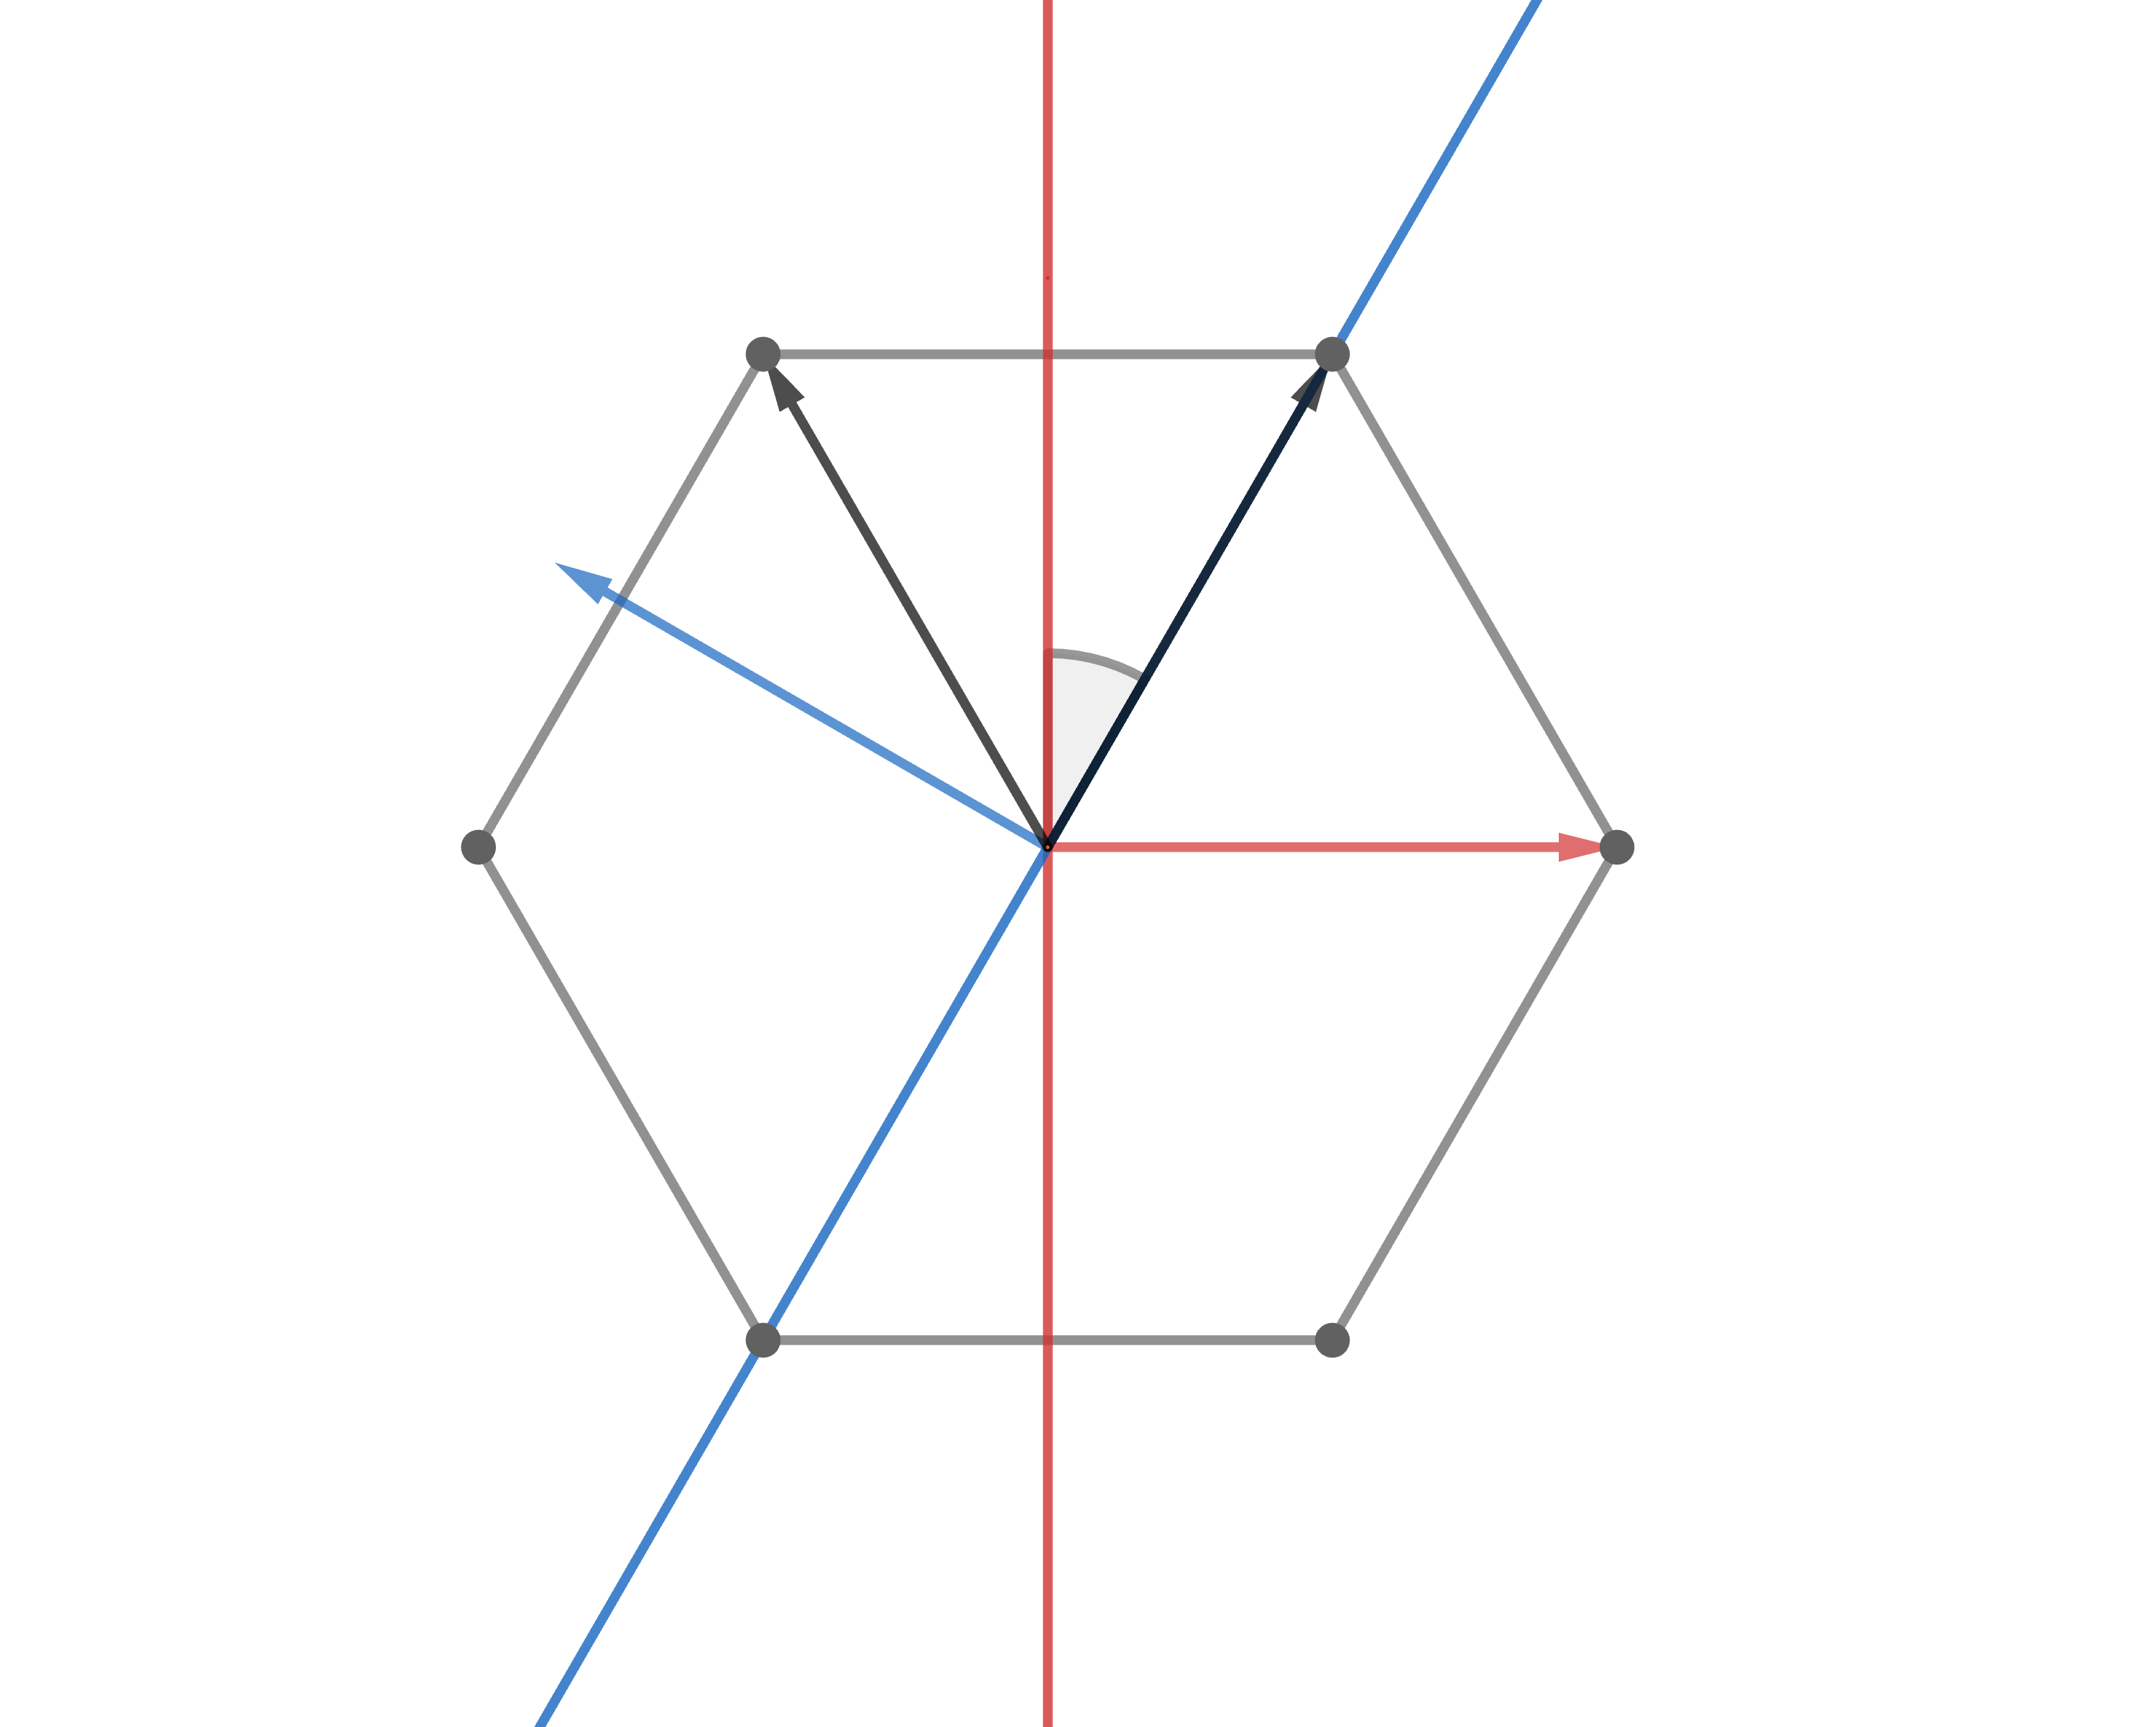
\includegraphics[width=5cm]{gfx/the dihedral proof case.png}
% \end{figure} % TODO: fix the image


% ***********************************************
\section{The fundamental domain and Stabilizers}
% ***********************************************

In this section, we will prove that the fundamental chamber \(C\subset V^*\) is indeed a fundamental domain for the action of \(W\) on its Tits cone \(WC\).
Moreover, we will work out how stabilizers of points look like and then show that the Tits cone is really a convex cone in the dual space \(V^*\).

We start by translating the results of the previous section to the language of chambers and halfspaces.
The following two lemmas capture this essence.

\begin{lemma}\label{lem:translation}
    Let \(w\in W\) and \(i\in I\).
    % Then the relation \(\ell(s_iw) > \ell(w)\) of \(s_i\) and \(w\) is equivalent to \(w(\mathring{C})\subset A_i^*\), \ie \(\;w\) leaving the open chamber inside the open halfspace, corresponding to \(s_i\).
    The relation \(\ell(s_i w) > \ell(w)\) is equivalent to saying that \(w\) leaves the open chamber \(\mathring{C}\) inside the open halfspace \(A_i^*\), corresponding to the generator \(s_i\).
    Put more formally, this states that the set \(w(\mathring{C})\) is a subset of the open halfspace \(A_i^*\).
\end{lemma}
\begin{proof}
    Observe that \(\ell(s_iw) > \ell(w)\) is equivalent to \(\ell(w^{-1}s_i) > \ell(w^{-1})\).
    Then by by \Cref{thm:action}, we have that \(w^{-1}(e_i) > 0\).
    Take an arbitrary point \(\varphi\in \mathring{C}\) in the open fundamental chamber, then we have that \(w(\varphi)(e_i) = \varphi(w^{-1}(e_i))\).
    Since the chamber \(C\) lies in \(A_i^*\) for all \(i\in I\) and \(\varphi \in \mathring{C}\), we see that \(w(\varphi) > 0\) is equivalent to \(w^{-1}(e_i)>0\).
    But this is true by assumption and since \(\varphi\) is arbitrary, we conclude that \(w(\mathring{C}) \subset A_i^*\).
\end{proof}

Of course this lemma also has a corresponding converse result as in the previous section.
% If we choose in the above lemma \(\widetilde{w} := s_iw\) for an \(i \in I\), we get
% \[\ell(s_i\widetilde{w}) = \ell(s_i^2 w) = \ell(w) > \ell(s_iw) = \ell(\widetilde{w}) \iff \widetilde{w}(C) = s_iw(C)\subset A_i^*.\]
% This is again equivalent to \(w(\mathring{C}) \subset s_i(A_i^*)\), and we have just proved the following lemma as the counterpart to \Cref{lem:translation}.

\begin{lemma}\label{lem:translation2}
    Let \(w\in W\) and \(i\in I\).
    % Then the relation \(\ell(s_iw) < \ell(w)\) holds if and only if we have \(w(\mathring{C})\subset s_i(A_i^*)\), \ie \(\;w\) moves the open chamber into the open halfspace complementary to \(A_i^*\).
    The relation \(\ell(s_i w) < \ell(w)\) is equivalent to saying that \(w\) now moves the open chamber \(\mathring{C}\) inside the open halfspace, complementary to \(A_i^*\).
    More formally, this states that the set \(w(\mathring{C})\) is a subset of the open halfspace \(s_i(A_i^*)\), as the \(s_i\) permute \(A_i^*\) and its corresponding complementary halfspace.
\end{lemma}
\begin{proof}
    Take \(w' = s_i w\) for some \(i \in I\) and \(w \in W\) so that \(\ell(s_i w) > \ell(w)\).
    Then we have that the length of \(s_i w' = w\) is strictly smaller then then length of \(w'\).
    % Then we have that \(\ell(s_i w') = \ell(w) < \ell(s_i w) = \ell(w')\)
    By applying above lemma we get that \(w(\mathring{C}) \subset A_i^*\), which is equivalent to \(s_i w'(\mathring{C}) \subset A_i^*\).
    Apply \(s_i\) to both sides leaves us with \(w'(\mathring{C}) \subset s_i(A_i^*)\), which proves the lemma.
\end{proof}

Building onto this insight, we now want to study the action of parabolic subgroups on the Tits cone to get an understanding of the stabilizers of points.
To do so, decompose the fundamental chamber into subsets corresponding to the parabolic subgroups of \(W\) as follows.

\begin{definition}
    Given a parabolic subgroup \(W_J\) corresponding to \(J\subset I\), set
    \[C_J := \bigcap_{j\in J} H_j^* \cap \bigcap_{k\notin J} A_k^*.\]
    We call these the corresponding parabolic subsets (of the fundamental chamber).
\end{definition}

\begin{example}\label{ex:parabolicset} % TODO: add picture
    \begin{enumerate}
        \item When the set \(J\) is empty, the corresponding parabolic subset \(C_\emptyset\) coincides with the entire chamber \(C\).
              Conversely, when \(J\) contains all indices, \(C_J\) reduces to the singleton \(\{0\}\).
        \item If \(J\) is a proper subset of \(I\) with cardinality one, then the corresponding subset \(C_J\) coincides with a codimension-one face of the chamber \(C\).
    \end{enumerate}
\end{example}

\begin{theorem}\label{thm:stabilizer}
    Let \(w\in W\) and \(J, K \subset I\) be subsets.
    Then \(w(C_J)\cap C_K \neq \emptyset\) implies \(J = K\), \(w\in W_J\) and thus \(w(C_J) = C_J\).
    In particular, the isotropy groups of the sets \(C_J\) are the parabolic subgroups \(W_J\).
\end{theorem}
\begin{proof}
    Let \(w\in W\) and \(J, K\subset I\) be subsets, such that \(w(C_J)\cap C_K \neq \emptyset\).
    % We also proof this theorem by induction on \(\ell(w)\), with the base case \(\ell(w) = 0\) being trivial.
    The proof is by induction on the length of \(w\).
    The base case \(\ell(w) = 0\) is trivial, as then \(w\) is trivial.

    Assume that \(\ell(w) > 0\) and choose \(i\in I\), such that \(\ell(s_iw) < \ell(w)\).
    Writing \(w = s_i(s_iw)\), by \Cref{lem:translation2} we know that \(w\) moves the open chamber \(\mathring{C}\) into the open halfspace \(s_i(A_i^*)\), i.e. \(w(\mathring{C})\subset s_i(A_i^*)\).
    Now using the continuity of the group action, we note that \(w(C) \subset \overline{s_i(A_i^*)}\). %is a subset of \(\overline{s_i(A_i^*)}\).
    Recall that by definition, the fundamental chamber \(C\) lies in the halfspaces \(\overline{A_i^*}\) for all \(i \in I\).
    % Now we use the continuity of the action of \(W\) to get that \(w(C)\subset \overline{s_i(A_i^*)}\), which then implies that \(w(C)\cap C\subset H_i^*\).
    % This follows, since the (closed) fundamental chamber \(C\) by definition is a subset of \(\overline{A_i^*}\).
    Thus, we record that \(w(C) \cap C \subset H_i^*\) and since \(s_i\) fixes the corresponding \(H_i^*\) by definition, it fixes every point in the intersection of \(C\) and its translate \(w(C)\).
    Note that the sets \(C_J\) and \(C_K\) are subsets of the fundamental chamber \(C\) and therefore, \(s_i\) fixes every point in the non-empty set \(w(C_J)\cap C_K\).
    But if \(s_i\) fixes some point \(\varphi\) in \(C_K\), we calculate
    \[\varphi(e_i) = s_i(\varphi)(e_i) = \varphi(s_i(e_i)) = -\varphi(e_i) \implies \varphi(e_i) = 0 \iff \varphi\in H_i^*.\]
    We deduce \(i\in K\), respectively \(s_i\in W_K\).
    Using this together with the assumption, we get that \(s_iw(C_J)\cap C_K = s_i(w(C_J)\cap C_K)\) is non-empty.
    We apply the induction hypothesis to the element \(s_iw\), to see that \(J = K\) and \(s_iw\in W_J\).
    Finally, since \(s_i\in W_J = W_K\), we have that \(s_iw \in W_J\) implies \(w\in W_J\), proving the theorem.
\end{proof}

% For the next theorem we want to prove, we want to recall the following definition.
Before proceeding with proving that the fundamental chamber lives up to its name, we want to clearly state what is meant by a fundamental domain.

\begin{definition}
    Let \(G\) be a group, acting on a topological space \(X\).
    We call a closed subset \(F\subset X\) a \emph{(strict) fundamental domain}, if for each \(x\in F\) its orbit \(Orb(x)\) intersects \(F\) in exactly one point.
\end{definition}

Note that, by definition of the Tits cone \(WC\), every \(W\)-orbit of a point \(\varphi\in C\) meets the fundamental chamber \(C\) in at least one point, namely \(\varphi\).
Thus, it suffices to proof that each \(W\)-orbit meets \(C\) in at most one point, to prove the following theorem.

\begin{theorem}\label{thm:funddomain}
    The fundamental chamber is a fundamental domain for the action of the Coxeter group \(W\) on its Tits cone \(WC\), justifying its name.
\end{theorem}
\begin{proof}
    Assume that \(\varphi,\psi\in C\) lie in the same \(W\)-orbit, but in different parabolic subsets \(C_J\), respectively \(C_K\) of the fundamental chamber. %, for \(J,K\subset I\).
    Since they lie in the same orbit, there is a \(w\in W\) with \(\varphi = w(\psi)\).
    Thus, the intersection \(w(C_J)\cap C_K\) is non-empty and \Cref{thm:stabilizer} implies equality of \(J\) and \(K\), as well as \(w \in W_J\).
    We deduce \(\varphi = w(\psi) = \psi\).
    Thus, every \(W\)-orbit of a point \(\varphi\in C\) meets the fundamental chamber \(C\) at most in \(\varphi\), proving the theorem.
\end{proof}

Define a set \(\mathcal{C}\) as the union of all translates of possible parabolic subsets \(C_J\) \ie, define \(\mathcal{C}\) by
\[\mathcal{C} := \bigcup_{J \subset I} \bigcup_{w \in W/W_J} w(C_J).\]
We want to emphasize here that by \Cref{thm:stabilizer} the sets of the form \(w(C_J)\) in the Tits cone \(WC\) are all disjoint for different \(J \subset I\) and \(w\) ranging over the coset \(W/W_J\).
% Note that \Cref{thm:stabilizer} implies that this set forms a partition of the Tits cone as it shows that the sets of the form \(w(C_J)\) in \(\mathcal{C}\) are all disjoint for \(w\) in the coset \(W/W_J\) and \(J\) a subset of \(I\).
Thus, the sets of \(\mathcal{C}\) form a partition of the Tits cone.
This decomposition (altough not into chambers) is a key component in the following theorem.

\begin{theorem}\label{thm:convexity}
    The Tits cone \(WC\) is a convex cone, and every closed line segment in the Tits cone meets only finitely many of the sets in \(\mathcal{C}\).
\end{theorem}
\begin{proof}
    First note that the fundamental chamber is a convex cone as the intersection of the finitely many closed halfspaces \(\overline{A_i^*}\).
    This implies that the Tits cone is a cone as well.
    We will prove the convexity by showing that every closed segment between any two points in the Tits cone is contained in it.
    Furthermore, we will prove that these segments can be covered by finitely many of the sets in the above defined union \(\mathcal{C}\), implying latter statement.

    Consider the closed segment \([\varphi, \psi]\) with \(\varphi, \psi \in WC\) and assume the endpoints lie in different chambers. % \(\varphi\in C\) and \(\psi\in w(C)\) for some \(w\in W\), i.e. the endpoints lie in different chambers.
    Proceed by induction on the word length \(\ell(w)\). %with the base case \(\ell(w) = 0\) implying \(\varphi,\psi\in C\).
    The base case \(\ell(w) = 0\) reduces to \(\varphi, \psi \in C\).
    Since \(C\) is convex and can trivially be covered by finitely many of the \(C_J\), this case has been dealt with.
    
    Therefore, we now assume \(\ell(w) > 0\).
    Intersect the segment \([\varphi, \psi]\) with the fundamental chamber \(C\), to receive two new segments \([\varphi, \xi]\) and \([\xi, \psi]\) (cf. \Cref{img:path}).
    % Note that we can divide the segment \([\varphi, \psi]\) into two parts, by intersecting it with the closed chamber \(C\) to get a closed segment \([\varphi, \xi]\) inside \(C\) and a segment \([\xi, \psi]\).
    The first segment can be covered by finitely many of the sets in \(\mathcal{C}\), as it lies inside the fundamental chamber \(C\).
    Thus, we need to show that we can cover the second segment \([\xi, \psi]\) by finitely many of these sets.
    Assume further, we have a \(J \subset I\), such that \(\psi\in s_i(A_i^*)\) for an \(i\in J\) and \(\psi\in\overline{A_i^*}\) for all \(i\notin J\).
    Then we have that \(\psi\notin C\).
    \Claim{1}{\(\xi\) has to lie in one of the codimension-one faces \(H_i^*\), \(i\in J\).}
    \Claimproof{1}{
        Assume that \(\xi\) lies in the open halfspace \(A_i^*\) for some \(i\in J\).
        Then every point \(\zeta\) in the intersection of a neighborhood of \(\xi\), contained in \(A_i^*\), with the segment \([\xi,\psi]\) has to also lie in \(A_i^*\). % for \(i\in J\). % and \(\zeta\in \overline{A_i^*}\) for \(i\notin J\).
        Clearly, \(\zeta\in\overline{A_i^*}\) for \(i\notin J\) holds as well, implying that \(\zeta\in C\).
        But this is a contradiction to the decomposition of the initial segment \([\varphi, \psi]\).
        Thus, \(\xi\) has to lie in one of the \(H_i^*\).
    }
    Using the assumptions \(\psi\in s_i(A_i^*)\) and \(\psi\in w(C)\), we deduce \(w(C)\subset \overline{s_i(A_i^*)}\), hence by continuity of the action \(w(\mathring{C})\subset s_i(A_i^*)\).
    By \Cref{lem:translation2} this is equivalent to \(\ell(s_iw) < \ell(w)\) and we are set up to apply the induction hypothesis to \(\xi\) and \(s_i(\psi)\in s_iw(C)\).
    This produces a cover of \([\xi,s_i(\psi)]\) by finitely many sets in \(\mathcal{C}\).
    But since we established that \(\xi\) has to lie in \(H_i^*\), translation by \(s_i\) gives \([s_i(\xi), s_i^2(\psi)] = [\xi, \psi]\), and thus we can cover this segment by finitely many sets as well.
    The result follows.
\end{proof}

\begin{figure}[ht]
    \centering
    \subfloat[\centering A path through the Tits cone.]{{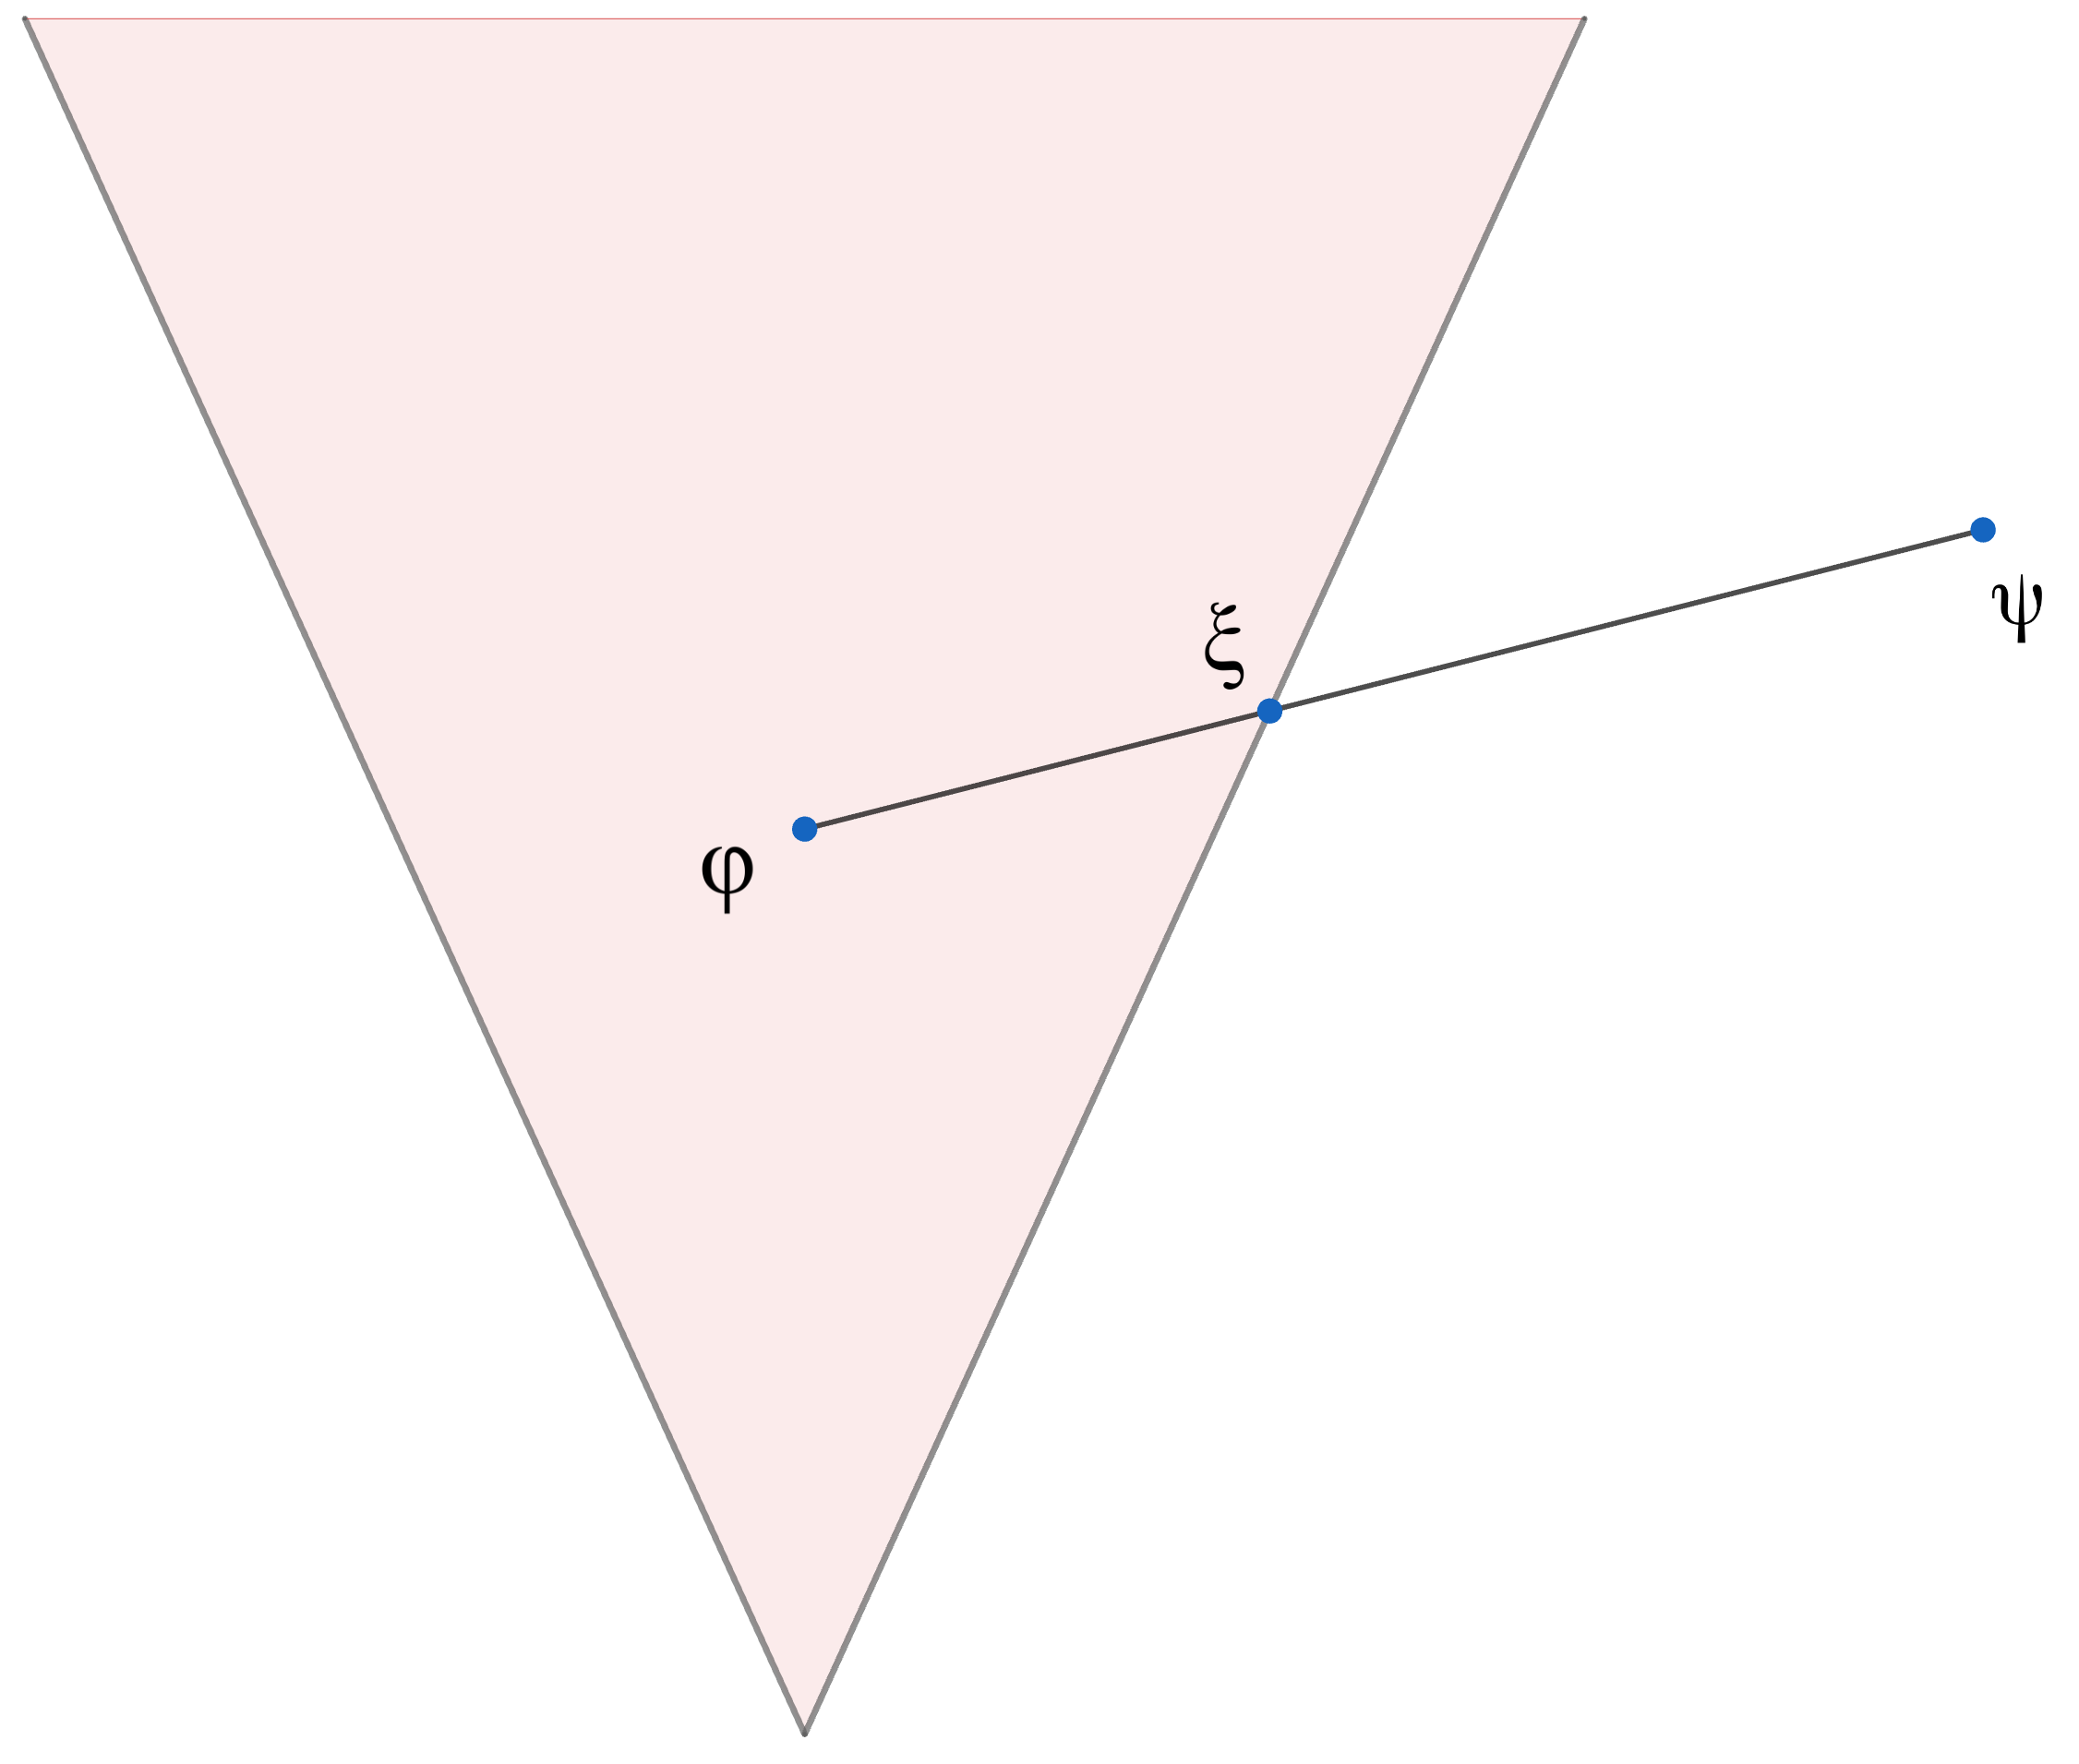
\includegraphics[width=5cm]{gfx/pfad durch kegel.png}}\label{img:path}}
    \qquad
    \subfloat[\centering A neighborhood of \(\xi\).]{{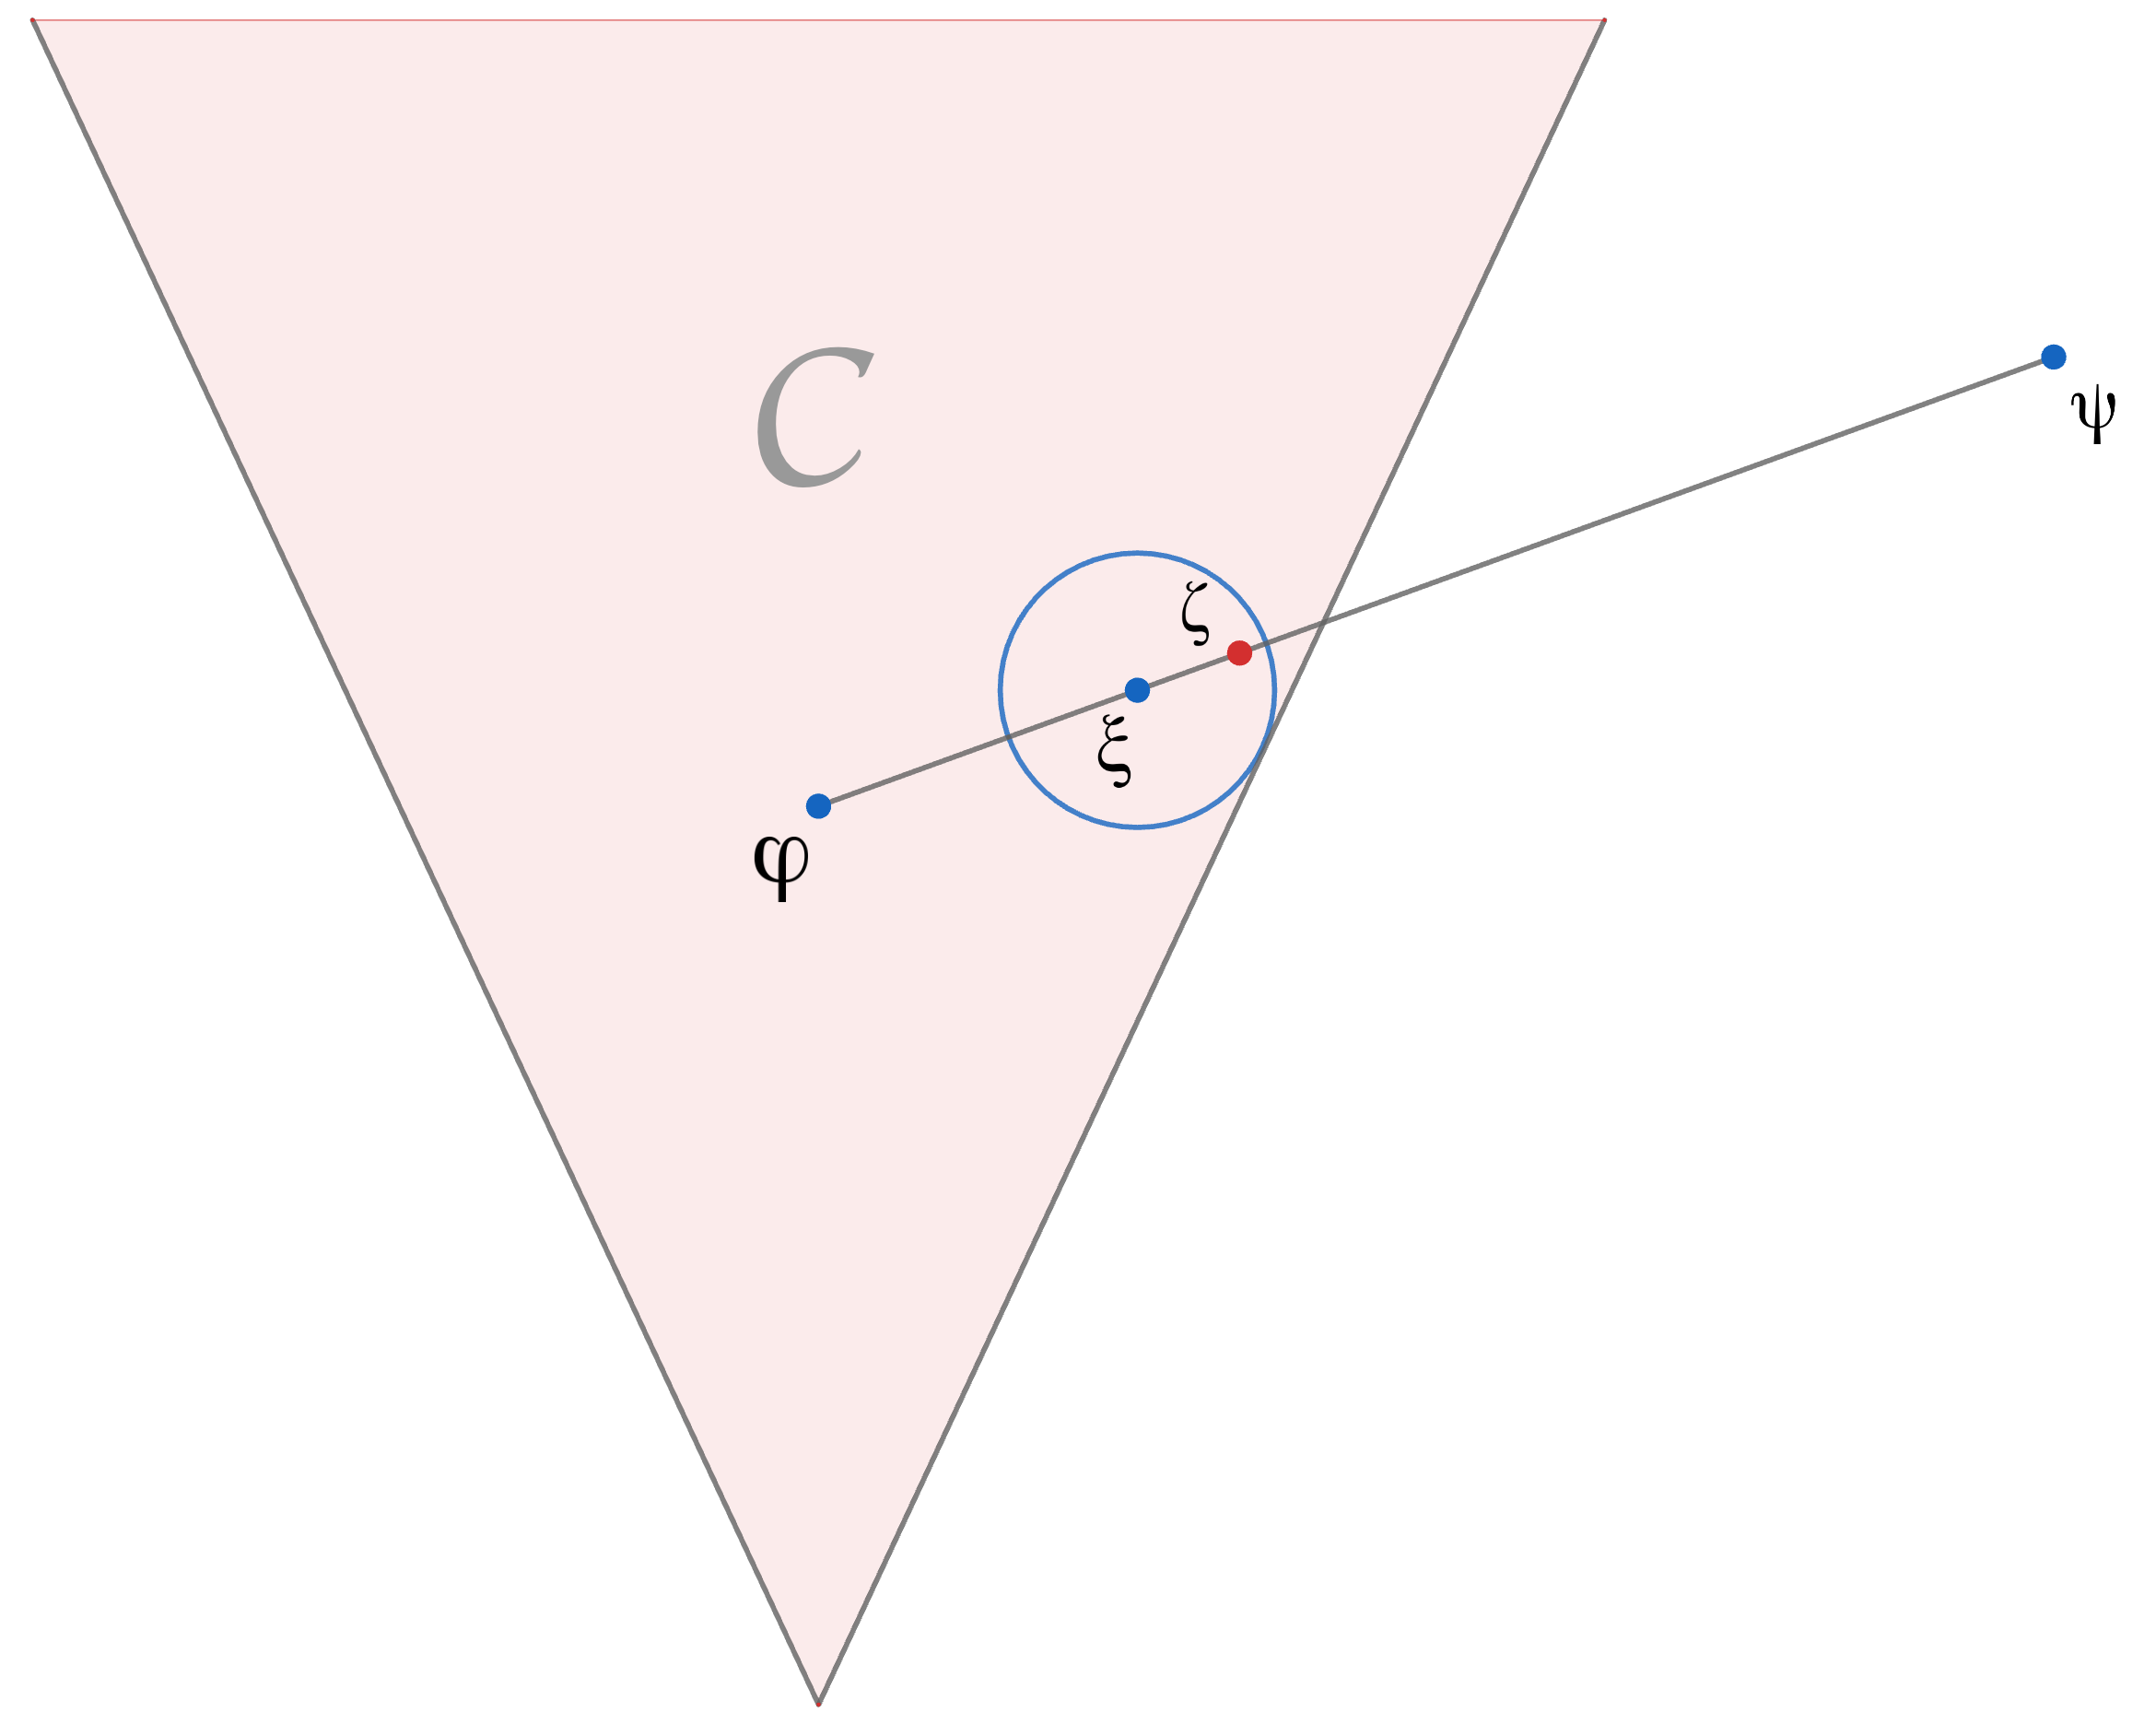
\includegraphics[width=5.35cm]{gfx/the neighborhood.png}}}
    % \caption{The picture to the proof.}
\end{figure}

To summarize, the essence of this section is that first of all the fundamental chamber is indeed a fundamental domain of the action of a Coxeter group on its Tits cone.
This was shown in \Cref{thm:funddomain}.
Furthermore, we want to emphasize that each point in the interior of the fundamental chamber has trivial stabilizer, which is a direct consequence of \Cref{thm:stabilizer}.
Moreover, every point in a parabolic subset \(C_J\) of \(C\), for \(J\) a subset of \(I\), is stabilized by the corresponding parabolic subgroup \(W_J\).

% An essential fact we want to emphasize here is that the stabilizer of the fundamental chamber is trivial.
% Setting \(J=K=\emptyset\), we obtain from \Cref{thm:stabilizer} (using that \(C_\emptyset = C\)), that if \(wC\cap C \neq \emptyset\) we must have \(w\in W_\emptyset = \{1\}\).
% Setting \(J=\emptyset\), we obtain from \Cref{thm:stabilizer} that the stabilizer subgroup of \(C_J = C_\emptyset = C\) (cf. \Cref{ex:parabolicset}) is precisely the parabolic subgroup \(W_J = W_\emptyset = \{1\}\).


% ***********************************************
\section{Covering actions - A Toolbox}
% ***********************************************

In this section we will assemble a set of tools, mostly coming from algebraic topology, connecting group actions to the notion of coverings.
They will be somewhat essential in the proof of the main theorem in the next chapter.
We start by saying what is meant by a covering.

\begin{definition}\label{def:covering}
    Let \(X, Y\) be topological spaces.
    A continuous map \(p: Y\to X\) is a \emph{covering map} and \(Y\) a \emph{covering space} for \(X\), if every point \(x\) in \(X\) has an open neighborhood \(U\), such that the preimage of \(U\) under \(p\) is a disjoint union of open sets \(U_i\) in \(Y\) for an index set \(I\).
    Furthermore, the map \(p\) has to be a local homeomorphism, meaning the restriction of \(p\) to the \(U_i\) is a homeomorphism onto its image \(p(U_i)\).
    Then, \(U\) is called \emph{evenly covered} and \(\vert I \vert\) the degree of the covering, while the open sets \(U_i\) are called the \emph{sheets} over \(U\) and the preimage of an \(x\) in \(X\) is called a \emph{fiber} of \(x\).
\end{definition}

It turns out that restricting the action of a group on a topological space in the right way will give coverings by quotienting out the action.
We make this precise in the following.

\begin{definition}
    Let \(G\) be a group, acting on a space \(X\).
    The action is said to be \emph{properly discontinuous}, if every point in \(X\) has a neighborhood \(U\) such that the set \(\{g\in G\;\vert\; g(U)\cap U \neq \emptyset\}\) is finite.
\end{definition}

\begin{definition}
    Let \(G\) be a group, acting on a space \(X\).
    The action is said to be a \emph{covering (space) action} if every point has a neighborhood \(U\) such that the set \(\{g\in G \;\vert\; g(U)\cap U \neq \emptyset\}\) consists only of the neutral element.
\end{definition}

Obviously, this last condition is even more restrictive.
Yet, at least for Hausdorff spaces, there is a connection between the two.
In addition to acting properly discontinuously, we have to demand the action to be free.

\begin{lemma}
    Let \(G\) be a group that acts freely and properly discontinuously on a Hausdorff space \(X\).
    Then the action of \(G\) is a covering action in the above sense.
\end{lemma}
\begin{proof}
    Let \(X\) be a Hausdorff space and \(G\) be a group acting freely, properly discontinuously on \(X\).
    Then for an open neighborhood \(U\) of \(x\in X\), the set \(M := \{g \in G \;\vert\; gU \cap U \neq \emptyset\}\) is finite.
    For these \(g \in M\) we pick pairwise disjoint Neighborhoods \(V_g\) of \(gx\), which is possible since \(X\) is Hausdorff and \(G\) acts freely (thus \(gx \neq x\)).
    Finally, set \(V = \left(\bigcap_{g \in M} g^{-1} V_g \right) \cap U\), which is open as finite intersection of open sets and by definition a neighborhood of \(x\).
\end{proof}

To finally construct coverings from group actions and connect them in some sense, we need a last condition on the space the group acts on.

\begin{definition}
    A path-connected topological space \(X\) is called \emph{simply connected}, if \(\pi_1(X)\cong \{1\}\).
\end{definition}

\begin{lemma}\label{lem:covering}
    Let \(G\) be a group, acting by a covering action on a simply connected topological space \(X\).
    Then the quotient map \(p_G:(X, x_0)\to (G\backslash X, Orb(x_0))\) is a covering map and \(\pi_1(G\backslash X, Orb(x_0))\cong G\).
\end{lemma}
\begin{proof}
    Let \(U\) be an open neighborhood of \(x\in X\), such that \(\{g \in G \;\vert\; gU \cap U \neq \emptyset\} = \{1\}\).
    \Claim{1}{The map \(p_G\) restricted to \(U\) is a continuous bijection onto its image \(p_G(U)\).}
    \Claimproof{1}{
        \begin{itemize}
            \item Continuity: \(V\subset G\backslash X\) is open if and only if \(p_G^{-1}(V)\) is open and thus \(p_G\) is continuous.
            \item Surjectivity: Since orbits of points are non-empty, \(p_G\) is surjective.
            \item Injectivity: Assume \(x,y \in X\) distinct with \(p_G(x) = p_G(y)\).
                But then there is a non-trivial element \(g \in G,\; g \neq 1_G\) with \(gx = y\), implying \(g(U) \cap U \neq \emptyset\).
                This is a contradiction to \(G\) acting by a covering action.
        \end{itemize}\vspace*{-2\parskip}
    }\vspace*{-2\parskip}
    \Claim{2}{Every point \(Orb(x) \in G\backslash X\) has a neighborhood \(V \subset G \backslash X\) with \(p_G^{-1}(V) = \bigsqcup_{g \in G} gU\).}
    % \Claim{2}{Every point \(Orb(x) \in G\backslash X\) has a neighborhood \(V := p_G(U)\), \(U\) as in \emph{Claim 1}, hence \(p_G^{-1}(V) = \bigsqcup_{g \in G} gU\).}
    \Claimproof{2}{
        By assumption the sets \(gU\) are all disjoint neighborhoods of \(gx \in X\) for all \(g \in G\).
        Moreover, for \(V := p_G(U) \subset G\backslash X\), we have \(p_G^{-1}(V) = \bigsqcup_{g \in G} gU\), proving the Claim.
    }\vspace*{-2\parskip}
    \Claim{3}{The map \(p_G\vert_{gU} \to V = p_G(U)\) is a homeomorphism for all \(g \in G\).}
    \Claimproof{3}{
        Note that the action of \(G\) on \(X\) is by homeomorphisms and \(U \subset X\) is open.
        Then the union \(\bigsqcup_{g \in G} gU\) is open as well and since \(p_G^{-1}(V) = \bigsqcup_{g \in G} gU\), the set \(V\) is open in the quotient topology of \(G \backslash X\).
        Therefore, the map \(p_G\) restricted to \(gU\) for \(g \in G\) is an open map and hence, by \emph{Claim 1} a homeomorphism.
    }
    Now all conditions in \Cref{def:covering} are satisfied, so \(p_G\) is a covering map.
    For the last part of the statement, note that \(X\) is simply connected, implying that it is the universal cover of \(G \backslash X\). %\(\faktor{X}{G}\).
    By definition, \(G\) is the group of Deck transformations, thus \(\pi_1(G \backslash X, Orb(x_0)) \cong G\).
    % For the last part of the statement, take a homotopy class of loops \([\gamma] \in \pi_1(G \backslash X, Gx_0)\) with representative \(\gamma\).
    % Define a map \(\varphi : \pi_1(G, x_0) \to G\) on homotopy classes \([\gamma]\), such that \(\varphi([\gamma])\) takes \(\widetilde{\gamma}(0) = x_0\) to \(\widetilde{\gamma}(1)\), where \(\widetilde{\gamma}: [0,1] \to X\) is a lift of \(\gamma\).
    % Now if \(\gamma'\) is another representative of \([\gamma]\) then, \(\widetilde{\overline{\gamma}'\cdot \gamma}\) is the lift of a contractible curve in \(G \backslash X\).
\end{proof}

%************************************************
\chapter{The main theorem}
%************************************************

Let us quickly recall the main theorem we want to prove.

\begin{theorem*}
    A finitely generated right-angled Coxeter group \(W\) has a finite index subgroup \(W'\) such that \(W'\) is residually finite and rationally solvable (RFRS).
\end{theorem*}

For the following, we consider the Tits cone \(WC\) corresponding to \(W\), living in \(\R^n\) for \(n = \abs{I}\).
Before continuing, we want to shortly mention that the fundamental chamber \(C\) has a natural orbifold structure as the quotient \(\faktor{WC}{W}\). % \(WC/W\).
This will be covered later on in slightly greater detail.
% By the discussion of last chapter, we know that by taking the quotient \(WC/W\), we are left with the fundamental chamber \(C\).
In the first section, our goal is to produce a manifold cover \(C' \to C\) of the fundamental chamber.
This cover will be induced by a finite index subgroup in the right-angled Coxeter group \(W\).


% ***********************************************
\section{Construction of the manifold cover}
% ***********************************************

Consider the abelianization \(W_{\text{ab}}\) of \(W\), which is isomorphic to \((\Z/2\Z)^{n}\).
Now, the abelianization yields a homomorphism \(\alpha : W \to W_{\text{ab}}\) to whose kernel \(\ker\alpha\), we will turn our attention to in the following.
Note that by the first homomorphism theorem, \(\ker\alpha\) has finite index in \(W\), since
\[\abs{\faktor{W}{\ker\alpha}} = \abs{\faktor{\Z}{2\Z}}^{n} = 2^{n} < \infty.\]
Here we used the fact that \(W\) is finitely generated, whence \(n = \abs{I} = \abs{S} < \infty\).

Furthermore, note that for each \(J \subset I\) with \(W_J\) finite, we have an isomorphism between \(W_J\) and \((\faktor{\Z}{2\Z})^{\abs{J}}\).
Thus, the restriction of \(\alpha\) to each such subgroup \(\alpha\vert_{W_J}\) is an injective homomorphism.
We now use that in the right-angled case, the isotropy subgroups of codimension-\(k\) faces are all of this form.
This can be seen, as the isotropy subgroup of a codimension-\(k\) face \(F\) is generated by the reflections in the \(k\) codimension-\(1\) faces, whose intersection forms \(F\).
As all these codimension-\(1\) faces meet at angle \(\frac{\pi}{2}\), the generators commute pairwise.
Therefore, all isotropy subgroups inject into the abelianization of \(W\).
This implies that the intersection of an isotropy subgroup with the kernel of \(\alpha\) is trivial and consequently no isotropy group is contained in the kernel \(\ker\alpha\).
Since finite subgroups are contained in isotropy subgroups, the kernel \(\ker\alpha\) acts freely on the Tits cone \(WC\) corresponding to \(W\).

In particular, by \Cref{thm:stabilizer} the action of \(W\) on the interior of its Tits cone \(int(WC)\) is properly discontinuously and by \Cref{thm:convexity} the Tits cone is also a convex cone, implying that it has trivial fundamental group.
Having all this information, we are able to apply \Cref{lem:covering} to obtain the covering
\[int(WC) \;\longrightarrow\; \faktor{int(WC)}{\ker\alpha} \qquad x \mapsto \text{Orb}_{\ker\alpha}(x).\]
Using the local homeomorphism property of a covering map and the fact that the Tits cone \(WC\) is a subspace of \(\R^n\), we conclude that the quotient \(\faktor{int(WC)}{\ker\alpha}\) is indeed a manifold.

% \begin{proposition}
    
% \end{proposition}


% ***********************************************
\section{Some orbifold theory}
% ***********************************************

In this section, we want to elaborate more on the natural orbifold structure of the fundamental chamber \(C\).
We start by giving a formal definition of an orbifold.
We break the definition down into smaller pieces, starting with local models, also called (orbifold) charts.

\begin{definition}
    A \emph{local model} is a pair \((\widetilde{U}, \Gamma)\), where \(\widetilde{U} \subset \R^n\) is open and \(\Gamma\) is a finite subgroup of the group of diffeomorphisms of \(\widetilde{U}\), denoted \emph{diffeo}\((\widetilde{U})\), acting on \(\widetilde{U}\).
    By abusing notation, we will sometimes say that the quotient \(U = \faktor{\widetilde{U}}{\Gamma}\;\) is the local model.
\end{definition}

Now that we defined a local structure of an orbifold, we want to translate between these local models.
This is being made precise by orbifold maps.

\begin{definition}
    An \emph{orbifold map} between local models \((\widetilde{U}_i, \Gamma_i), (\widetilde{U}_j, \Gamma_j)\) is a pair of maps \((\widetilde{\psi}, \varphi)\).
    The map \(\widetilde{\psi} : \widetilde{U}_i \to \widetilde{U}_j\) is smooth and \(\varphi : \Gamma_i \to \Gamma_j\) a homomorphism of groups, such that the map \(\widetilde{\psi}\) is \(\varphi\)-equivariant, meaning that for all \(g \in \Gamma_i\) and all \(\widetilde{x} \in \widetilde{U}_i\), \(\widetilde{\psi}(g\widetilde{x}) = \varphi(g)\widetilde{\psi}(\widetilde{x})\) holds.
    Then \(\widetilde{\psi}\) induces a map \(\psi : \faktor{\widetilde{U}_i}{\Gamma_i} \to \faktor{\widetilde{U}_j}{\Gamma_j}\), between the local models.
    When all three of these maps are injective, we call \(\psi\) a local isomorphism.
\end{definition}

Now that we have these local definitions, we `glue' them together, to obtain an orbifold.
Recall that a topological space is \emph{paracompact}, if 

\begin{definition}
    An \(n\)-dimensional \emph{(smooth) orbifold} \(Q\) is a pair \((X_Q, \mathcal{A})\).
    The space \(X_Q\) is a paracompact Hausdorff space, called the \emph{underlying space}.
    The set \(\mathcal{A}\) is called an \emph{orbifold atlas}, consisting of charts \((U_i, \phi_i)\), indexed by some set \(I\) and satisfying the following conditions:
    \begin{itemize}
        \item the \(U_i\) form an open cover of the underlying space \(X_Q\),\vspace*{-.7em}
        \item for each \(U_i\) there exists a local model \(\faktor{\widetilde{U}_i}{\Gamma_i}\) with a homeomorphism \(\phi_i : U_i \to \faktor{\widetilde{U}_i}{\Gamma_i}\) and
        \item charts have to be compatible, meaning that for \(U_i \subset U_j\) the inclusion is a local isomorphism.
    \end{itemize}
\end{definition}

To sketch the connection between manifolds and orbifolds, let us mention one more thing.

\begin{definition}
    The \emph{local group} \(loc(x)\) of some \(x\) in a local model \(\faktor{\widetilde{U}}{\Gamma}\;\) is the isotropy group of any \(\widetilde{x}\) in \(\widetilde{U}\), getting projected onto \(x\).
    The \emph{singular locus} \(\Sigma (Q)\) of an orbifold \(Q\) consists of all points in the underlying space \(X_Q\) with non-trivial local group, i.e. \(\Sigma(Q) = \{x \in X_Q \;\vert\; loc(x) \neq \{1\}\}\).
\end{definition}

By this definition, we see that an orbifold with empty singular locus is just a manifold.
Furthermore, when thinking about an orbifold, we can just think about the underlying space and label each element in the singular locus by its local group.

Many basic examples arise by taking the quotient relative to a properly discontinuous group action on \(\R^n\).
We want to mention at least some examples.

\begin{example}
    % \begin{enumerate}
    %     \item The cone as an orbifold \(C\): consider \(G \cong \Z/n\Z\) acting on \(X_C = \R^2\) by rotation about \(\frac{2\pi}{n}\) around the origin.
    %         The quotient \(\R^2 / G\) is a cone with cone angle \(\frac{2\pi}{n}\), with the only singular point the cone point.
    %     \item The `teardrop' orbifold \(T\): consider \(G \cong \Z/n\Z\) acting on \(X_T = S^2\) by rotation about \(\frac{2\pi}{n}\) around the north pole.
    %         The quotient \(S^2 / G\) is a `teardrop' with the only singular point the north pole.
    % \end{enumerate}
\end{example}

Many orbifolds arise by passing to the quotient \(M/G\) of a properly discontinuous action of a group \(G\) on a topological space \(M\).
This is also the case for the fundamental chamber \(C\), its natural orbifold structure arises by taking the quotient of the Tits cone of \(W\) by its action. % TODO: add picture

Another concept worth mentioning is the theory of orbifold coverings.

\begin{definition}
    An orbifold covering \(p: Q' \to Q\) is a continuous map on the underlying spaces \(X_{Q'} \to X_Q\), such that for each point \(x \in X_Q\) there is a local model \(U = \faktor{\widetilde{U}}{\Gamma}\) around \(x\) and each component \(V_i\) of \(p^{-1}(U)\) is homeomorphic to \(\faktor{\widetilde{U}}{\Gamma_i}\) for a subgroup \(\Gamma_i\) of \(\Gamma\).
    Furthermore, the restriction \(p\vert_{V_i} : V_i \to U\) corresponds to the natural projection \(\faktor{\widetilde{U}}{\Gamma_i} \to \faktor{\widetilde{U}}{\Gamma}\).
\end{definition}

% Recall that any manifold can be interpreted as an orbifold where every local model \(\;\faktor{\widetilde{U}}{\Gamma}\;\) has \(\Gamma\) to be the trivial group.
% Thus, let us interpret the manifold \(\faktor{WC}{\ker\alpha}\) as such an orbifold.


% ***********************************************
\section{The cofinal cover}
% ***********************************************

In this section, we want to at least \emph{sketch} the proof of the existence of a cofinal sequence of two-fold covers, arising by iteratively reflecting in faces.
Some more results from the theory of orbifolds are needed for the whole proof.
We will state and use them without proof.

The following proposition tells us, that for a right-angled Coxeter group, we are able to `double' the fundamental chamber in one of its faces and are still able to cover the whole Tits cone \(WC\) by reflecting in the faces of the resulting chamber.
By doubling, pictorially, we mean to unfold the fundamental chamber (more generally a polytope) along one of its faces, by reflecting in this face.
The chamber and its double will then be the new chamber of interest.

\begin{proposition}\label{prop:double}
    Let \(C \subset \R^n\) be the fundamental chamber of a right-angled Coxeter group \(W\), acting on its Tits cone \(WC\).
    The orbifold fundamental group \(\pi_1^{\text{orb}}(P)\) of the doubled chamber \(P\) is isomorphic to the reflection group generated by reflections in its faces.
    Further, it has index \(2\) in the orbifold fundamental group \(\pi_1^{\text{orb}}(C)\) of \(C\). %, due to the covering theory of orbifolds.
    This procedure can be iterated and the induced group action of \(\pi_1^{\text{orb}}(P)\) by reflections in the faces of the doubled polytope \(P\) on the Tits cone \(WC\) corresponding to \(W\) satisfies the following conditions
    \[g\mathring{P} \cap \mathring{P} \neq \emptyset \implies g = 1 \qquad \text{ and } \qquad \underset{g \in \pi_1^{\text{orb}}(P)}{\bigcup} gP = WC.\]
    % \begin{itemize}
    %     \item \(g\mathring{P} \cap \mathring{P} \neq \emptyset \implies g = 1\),
    %     \item \(\underset{g \in \pi_1^{\text{orb}}(P)}{\bigcup} gP = WC\).
    % \end{itemize}
\end{proposition}

To state the other helping lemma we will need, we first want to show that each chamber in the Tits cone can uniquely be labeled by elements of its corresponding group.

\begin{lemma}
    Let \(W\) be a Coxeter group and \(WC\) its Tits cone.
    The chambers of the form \(w(C)\) in the Tits cone can be labeled uniquely by elements in \(W\).
\end{lemma}
\begin{proof}
    Let \(v(C), w(C)\) be chambers in \(WC\) for \(v, w \in W\), such that \(v \neq w\) and \(w(C) = v(C)\).\newline
    But then, by \Cref{thm:stabilizer} we have that
    \[w(C) \cap v(C) = w(C \cap w^{-1}v(C)) \neq \emptyset \implies w^{-1}v = 1 \iff w = v.\]
    Thus, the chambers can be labeled in a unique way.
\end{proof}

We proceed with a helpful result, whose proof will be sketched.

\begin{lemma}
    Let \(C \subset \R^n\) be the fundamental chamber of a Coxeter group \(W\).
    The non-trivial labels \(w_i \neq 1_W\) of the chambers, defining the polytope \(P = \bigcup_{i=1}^n w_i C\), are \emph{not} contained in the reflection group, generated by reflecting in its faces.
\end{lemma}
\begin{proof}
    The idea is to produce a contradiction to \Cref{prop:double}. \newline
    Let \(w_i \neq 1_W\) be one of those labels.
    But then, \(w_i(\mathring{P}) \cap \mathring{P} \neq \emptyset\), contradicting said proposition.
\end{proof}

Using this insight, we define a graph \(G\) with vertices \(V(G) := \{w(C) \;\vert\; w \in W\}\) and edges \(E(G) := W \times S\).
The endpoint map is given by \(\delta : W \times S \to 2^{V(G)},\; (w, s) \mapsto (w(C), ws(C))\).
Thus, two vertices \(w(C)\) and \(v(C)\) have an edge, if there is an \(s \in S\), such that \(ws = v\).
Then, clearly we have \(wsw^{-1}w(C) = ws(C) = v(C)\).
Note that the element \(wsw^{-1}\) is the only element, that flips the edge \(\{w(C), ws(C)\}\).
Thus, the map \(W \times S \to W, \; (w, s) \mapsto wsw^{-1}\) defines a labeling of the edges by elements in \(W\).
We will call the combinatorial graph of \(G\) (meaning that every double edge gets collapsed) the \emph{chamber graph} Cham\((W, S)\) of \(W\).

It is obvious, that this graph is isomorphic to the combinatorial Cayley graph of the group \(W\) and we see that the Cayley graph `embeds' into the Tits cone \(WC\).
This will be useful to prove the next theorem.

\begin{theorem}
    By doubling in a face of the fundamental chamber and iteratively doubling the resulting chamber, we will at some point cover every chamber in the Tits cone \(WC\).
\end{theorem}
\begin{proof}
    The proof is by induction on the word length \(\ell(w)\).
    For \(\ell(w) = 0\), the corresponding chamber is the fundamental chamber \(C\), which is covered by itself.
    \IH{Chambers with labels \(v\) of length \(\ell(v) = k - 1\) are covered by a polytope \(P = \bigcup_{i=1}^n w_i(C)\).}\par\noindent
    We need to show that chambers of the form \(w(C)\) with \(\ell(w) = k\) can be covered by reflecting in a face of the polytope \(P\).
    Using the chamber graph Cham\((W, S)\), constructed above, we deduce that for each such \(w\), there is a \(v \in W\) of length \(\ell(v) = k - 1\), connected to \(w\) by an edge in Cham\((W, S)\). % , labeled by \(ws_iw^{-1}\) for an \(i \in I\).
    This is due to the fact that the chamber graph is isomorphic to the Cayley graph of  \(W\) and the length function of \(W\) is induced by the Cayley graph.
    But then, the chamber \(w(C)\) is adjacent to the chamber \(v(C)\) and the latter is contained in \(P\) by \textbf{(IH)}.
    Thus, either \(w(C)\) itself is already contained in \(P\) or we reflect in the face shared by \(w(C)\) and \(v(C)\) to cover \(w(C)\) with the double \(P'\) of \(P\).
    Now, continuing with the next element \(w\) of length \(k\), we eventually double \(P'\) and repeat this for all such \(w\).
    This iterative doubling process is valid by \Cref{prop:double} and by induction every chamber \(g(C)\) for \(g \in W\) can be covered.
\end{proof}

\begin{figure}[ht!]
    \centering
    \subfloat[The fundamnetal chamber \(C\).]{{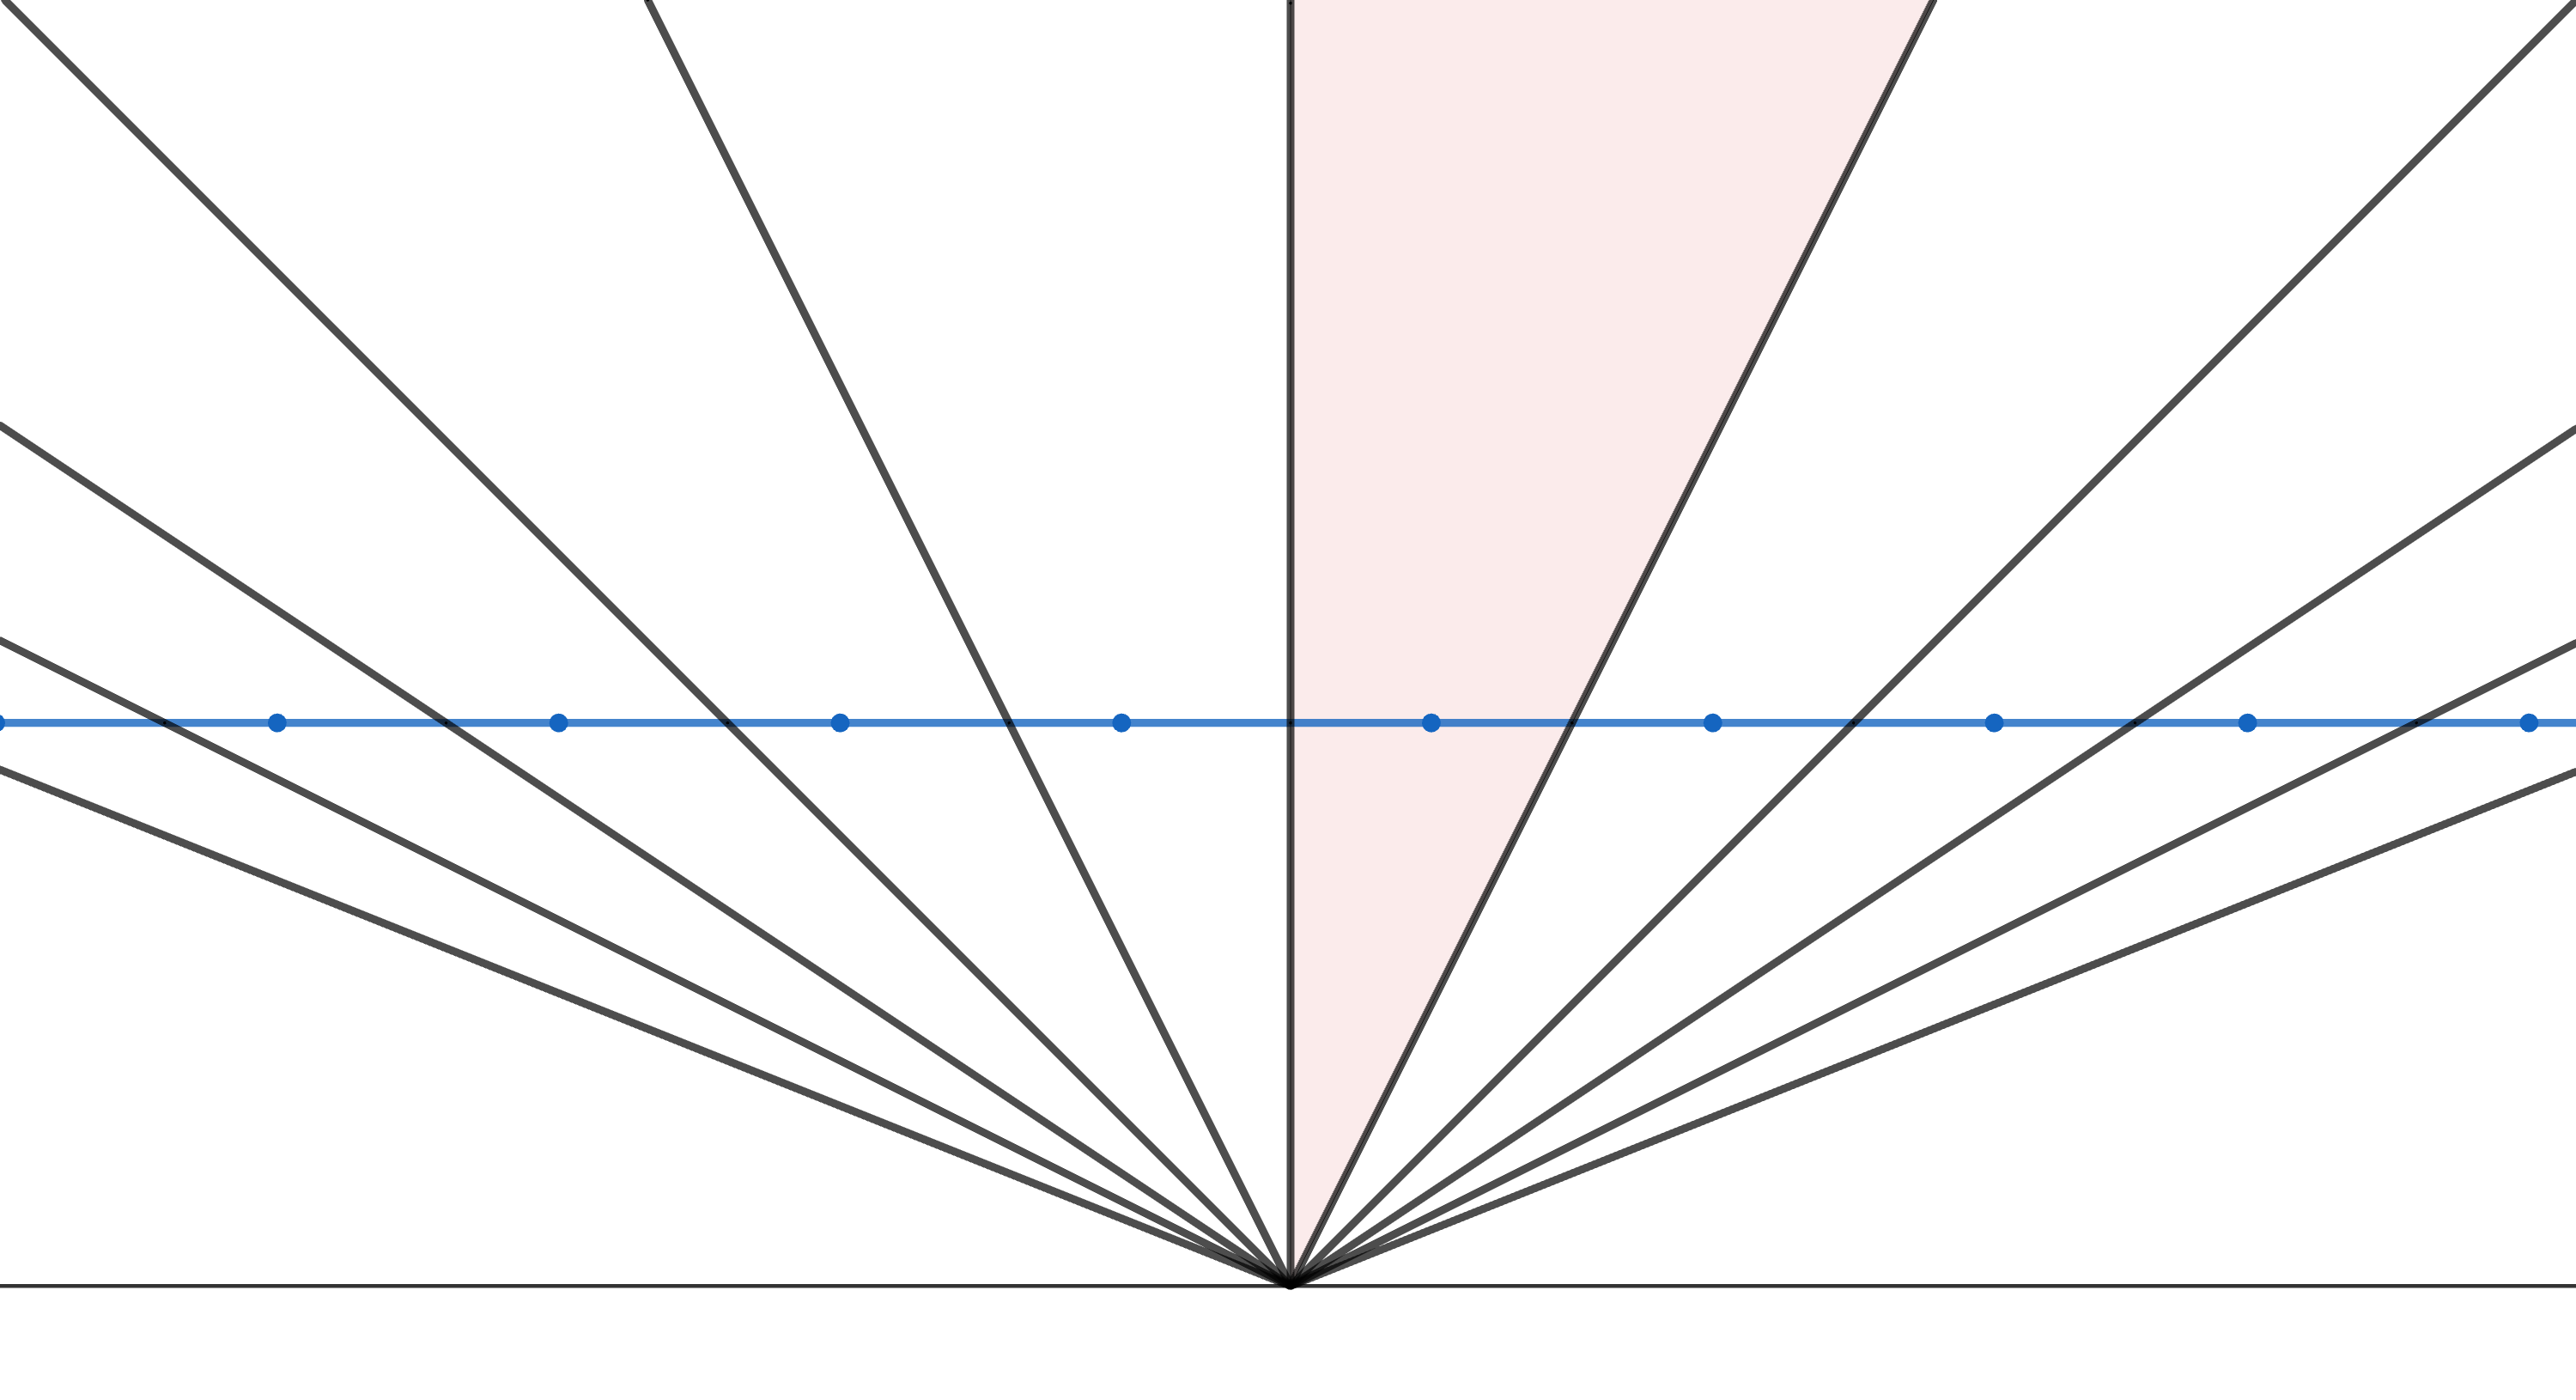
\includegraphics[width=7cm]{gfx/chamber graph - 1.png}}}\qquad
    \subfloat[The double polytope \(P = C \cup s_1(C)\)]{{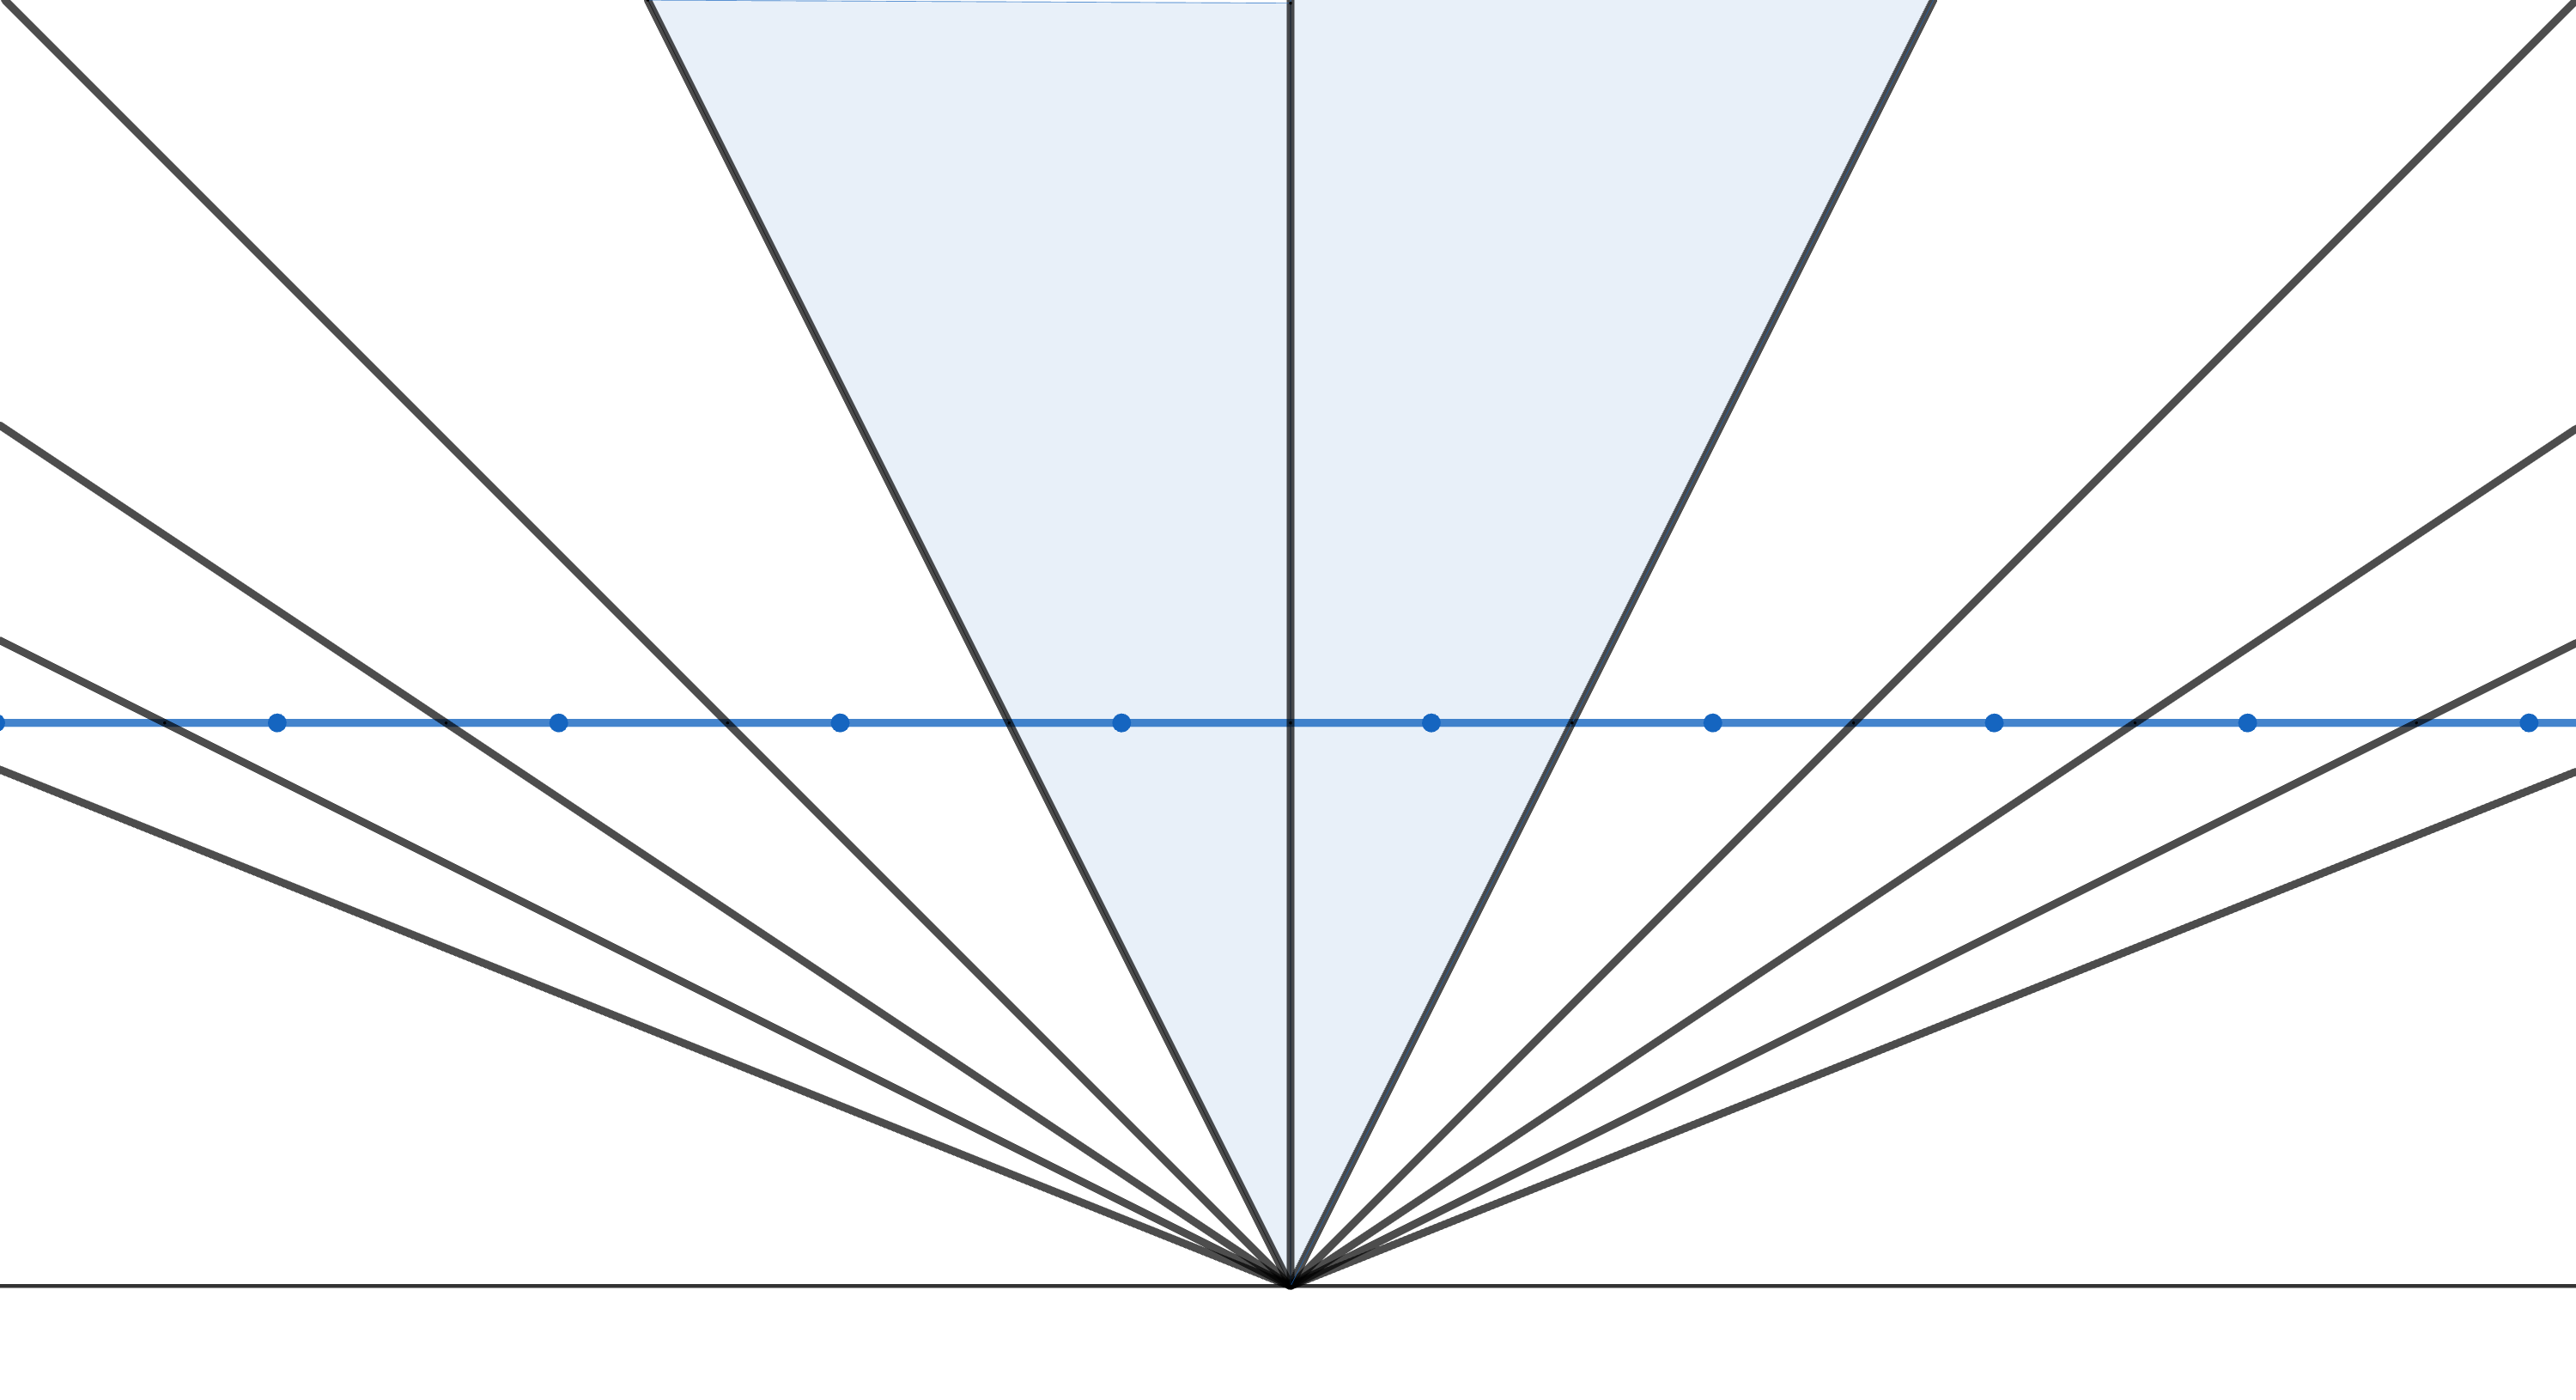
\includegraphics[width=7cm]{gfx/chamber graph - 2.png}}}\newline
    \subfloat[The double polytope \(P' = P \cup s_1s_2s_1(P)\)]{{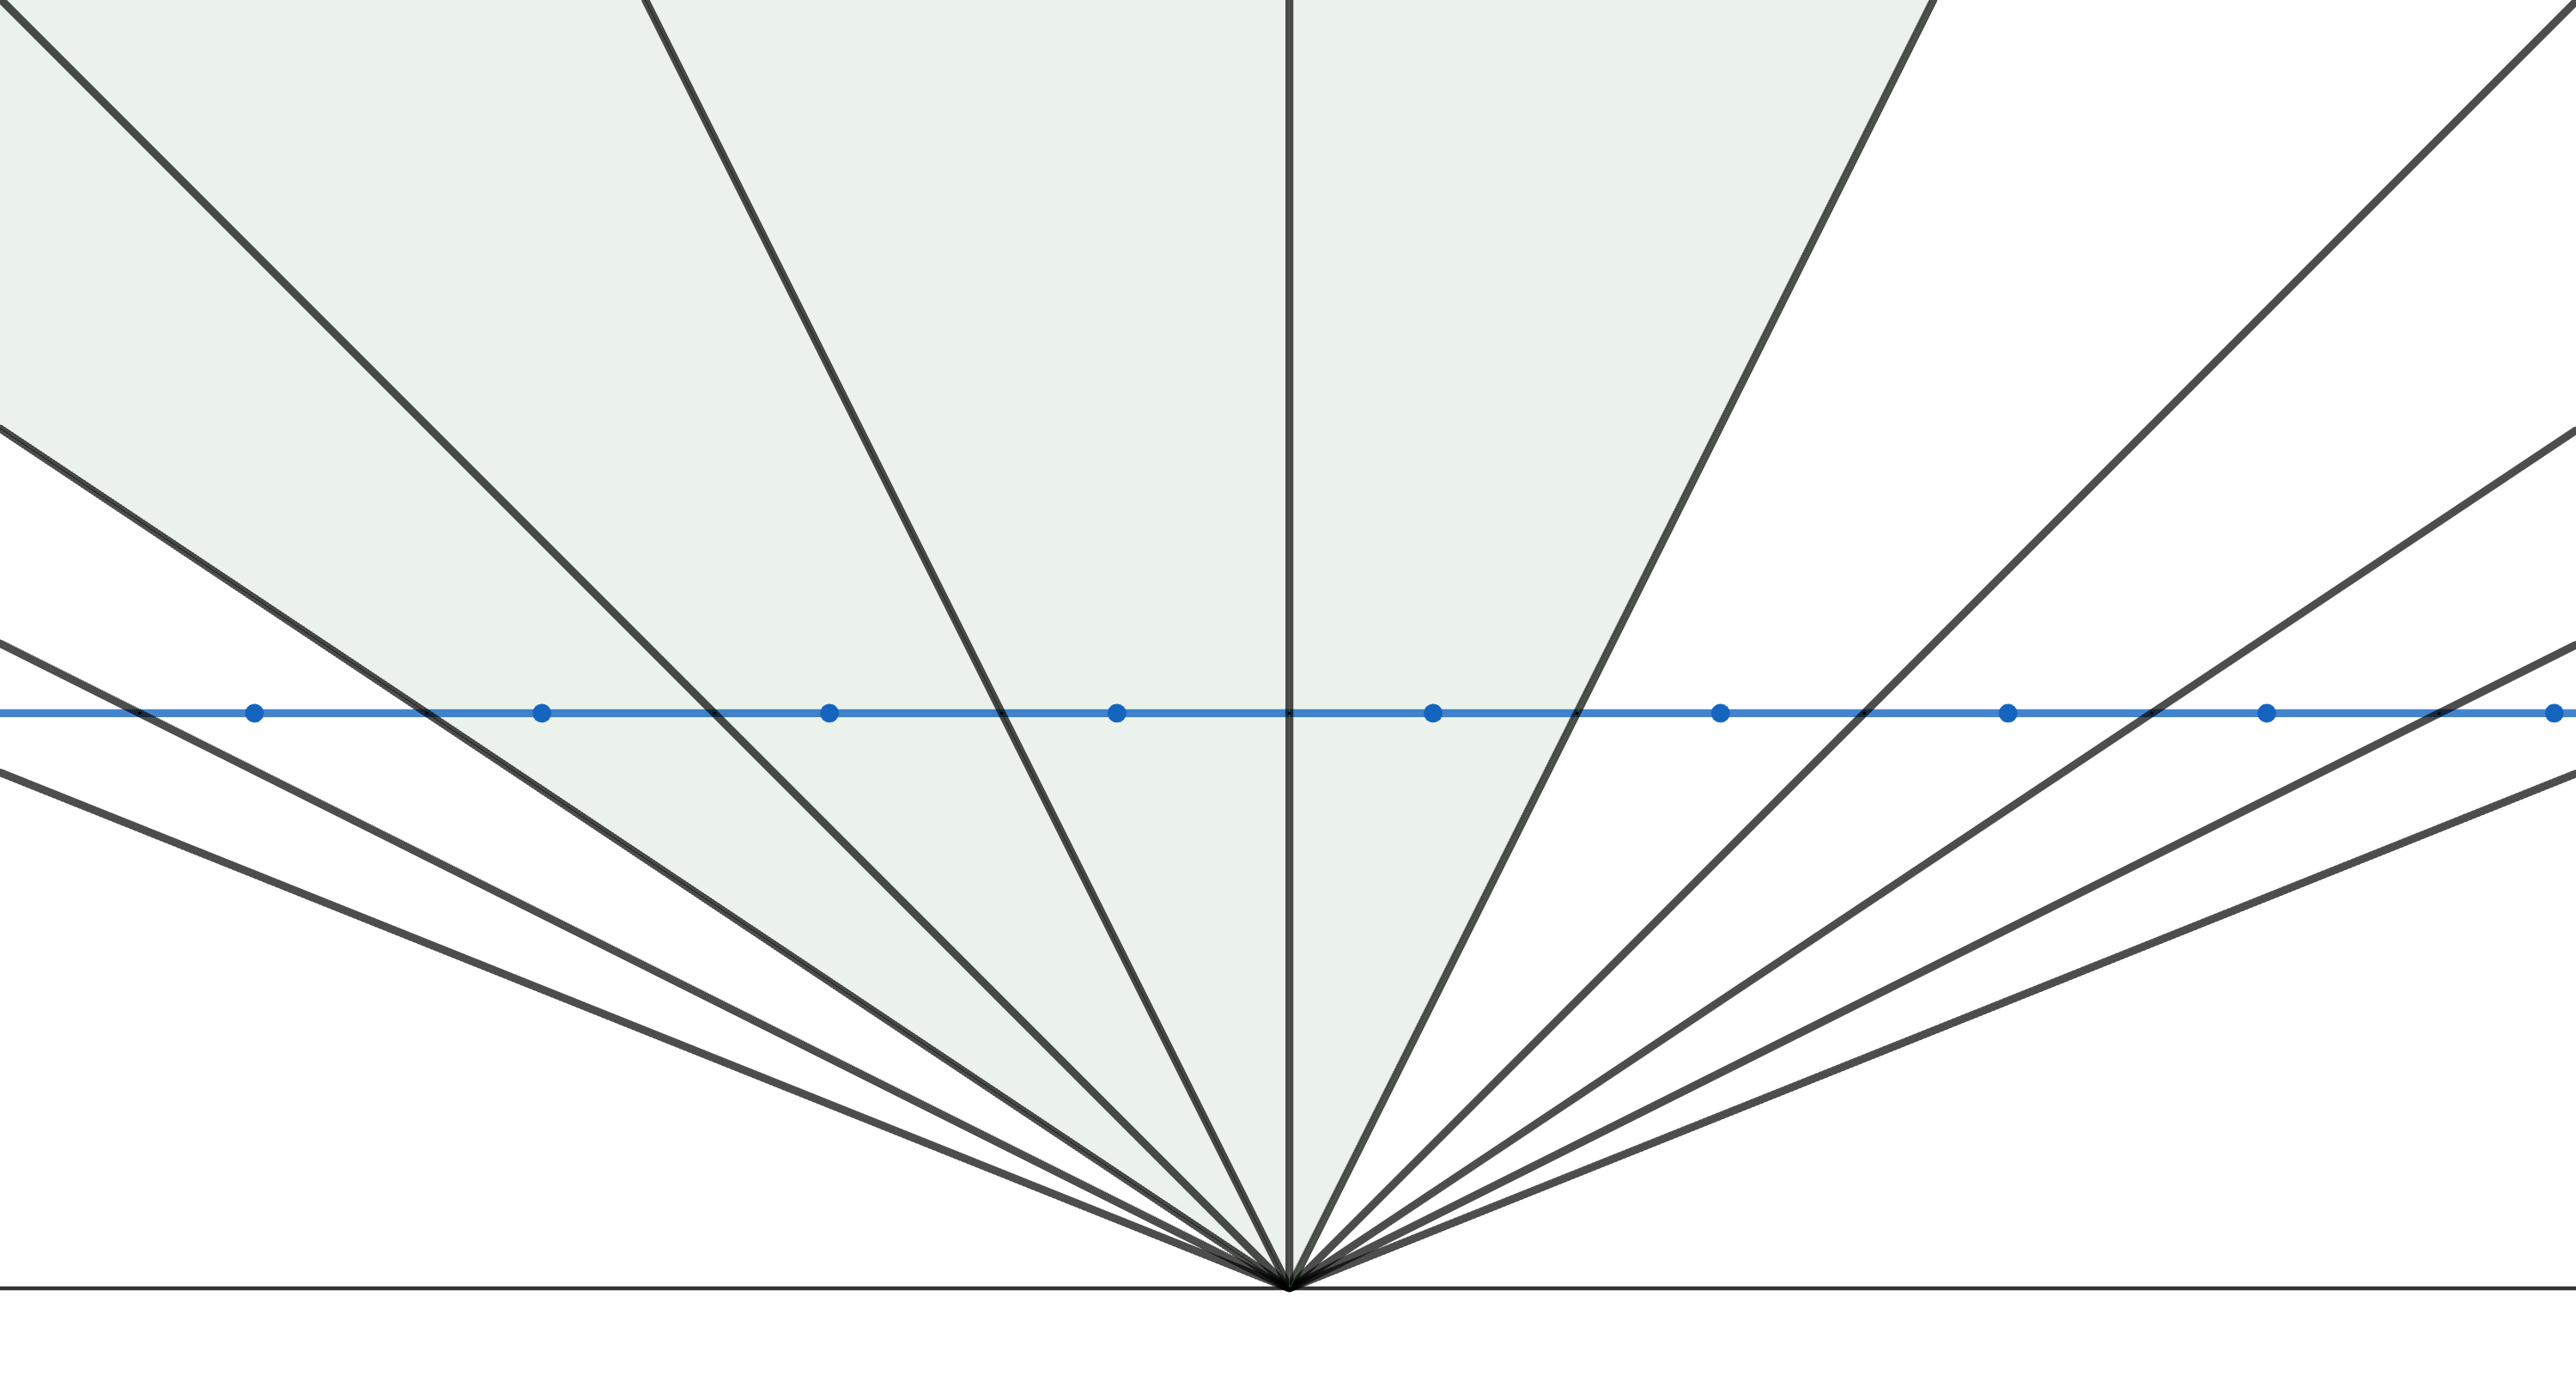
\includegraphics[width=7cm]{gfx/chamber graph - 3.png}}}
\end{figure}

% ********************************************************************
% Backmatter
%*******************************************************
% \appendix
%\renewcommand{\thechapter}{\alph{chapter}}
% \cleardoublepage
% \part{Appendix}
% %********************************************************************
% Appendix
%*******************************************************
% If problems with the headers: get headings in appendix etc. right
%\markboth{\spacedlowsmallcaps{Appendix}}{\spacedlowsmallcaps{Appendix}}
\chapter{Appendix Test}


%********************************************************************
% Other Stuff in the Back
%*******************************************************
\cleardoublepage%********************************************************************
% Bibliography
%*******************************************************
% work-around to have small caps also here in the headline
% https://tex.stackexchange.com/questions/188126/wrong-header-in-bibliography-classicthesis
% Thanks to Enrico Gregorio
\defbibheading{bibintoc}[\bibname]{%
    \phantomsection
    \manualmark
    \markboth{\spacedlowsmallcaps{#1}}{\spacedlowsmallcaps{#1}}%
    \addtocontents{toc}{\protect\vspace{\beforebibskip}}%
    \addcontentsline{toc}{chapter}{\tocEntry{#1}}%
    \chapter*{#1}%
}
\printbibliography[heading=bibintoc]

% Old version, will be removed later
% work-around to have small caps also here in the headline
% \manualmark
% \markboth{\spacedlowsmallcaps{\bibname}}{\spacedlowsmallcaps{\bibname}} % work-around to have small caps also
% \phantomsection
% \refstepcounter{dummy}
% \addtocontents{toc}{\protect\vspace{\beforebibskip}} % to have the bib a bit from the rest in the toc
% \addcontentsline{toc}{chapter}{\tocEntry{\bibname}}
% \label{app:bibliography}
% \printbibliography

% \cleardoublepage%*******************************************************
% Declaration
%*******************************************************
\pdfbookmark[0]{Declaration}{declaration}
\chapter*{Declaration}
\thispagestyle{empty}

\bigskip

\noindent\textit{\myLocation, \myTime}

\smallskip

\begin{flushright}
    \begin{tabular}{m{5cm}}
        \\ \hline
        \centering\myName \\
    \end{tabular}
\end{flushright}

% \cleardoublepage\pagestyle{empty}

\hfill

\vfill


\pdfbookmark[0]{Colophon}{colophon}
\section*{Colophon}
This document was typeset using the typographical look-and-feel \texttt{classicthesis} developed by Andr\'e Miede and Ivo Pletikosić.
The style was inspired by Robert Bringhurst's seminal book on typography ``\emph{The Elements of Typographic Style}''.
\texttt{classicthesis} is available for both \LaTeX\ and \mLyX:
\begin{center}
\url{https://bitbucket.org/amiede/classicthesis/}
\end{center}
Happy users of \texttt{classicthesis} usually send a real postcard to the author, a collection of postcards received so far is featured here:
\begin{center}
\url{http://postcards.miede.de/}
\end{center}
Thank you very much for your feedback and contribution.

\bigskip

\noindent\finalVersionString

%Hermann Zapf's \emph{Palatino} and \emph{Euler} type faces (Type~1 PostScript fonts \emph{URW
%Palladio L} and \emph{FPL}) are used. The ``typewriter'' text is typeset in \emph{Bera Mono},
%originally developed by Bitstream, Inc. as ``Bitstream Vera''. (Type~1 PostScript fonts were made
%available by Malte Rosenau and
%Ulrich Dirr.)

%\paragraph{note:} The custom size of the textblock was calculated
%using the directions given by Mr. Bringhurst (pages 26--29 and
%175/176). 10~pt Palatino needs  133.21~pt for the string
%``abcdefghijklmnopqrstuvwxyz''. This yields a good line length between
%24--26~pc (288--312~pt). Using a ``\emph{double square textblock}''
%with a 1:2 ratio this results in a textblock of 312:624~pt (which
%includes the headline in this design). A good alternative would be the
%``\emph{golden section textblock}'' with a ratio of 1:1.62, here
%312:505.44~pt. For comparison, \texttt{DIV9} of the \texttt{typearea}
%package results in a line length of 389~pt (32.4~pc), which is by far
%too long. However, this information will only be of interest for
%hardcore pseudo-typographers like me.%
%
%To make your own calculations, use the following commands and look up
%the corresponding lengths in the book:
%\begin{verbatim}
%    \settowidth{\abcd}{abcdefghijklmnopqrstuvwxyz}
%    \the\abcd\ % prints the value of the length
%\end{verbatim}
%Please see the file \texttt{classicthesis.sty} for some precalculated
%values for Palatino and Minion.
%
%    \settowidth{\abcd}{abcdefghijklmnopqrstuvwxyz}
%    \the\abcd\ % prints the value of the length


% ********************************************************************
% Game Over: Restore, Restart, or Quit?
%*******************************************************
\end{document}
% ********************************************************************
